% ROZDZIAŁ 29 -- podstawy geometrycznej teorii miary
\chapter[Prostowalność i zbiory o skończonym obwodzie]{Zbiory prostowalne, funkcje BV i zbiory o skończonym obwodzie}
\label{ch:geometric-measure-29}

\section{Cel i zakres teorii}
W geometrii różniczkowej badaliśmy gładkie podrozmaitości, ich
metryki indukowane oraz normalne. W tym rozdziale będziemy mierzyć
również brzegi zbiorów, które mają narożniki, pęknięcia lub
nieregularności i nie są podrozmaitościami. Zamiast zakładać
istnienie klasycznej normalnej w każdym punkcie, zdefiniujemy ją
\emph{miarowo}. Przygotujemy w ten sposób język geometrycznej
teorii miary, teorii wariacyjnej i równań różniczkowych cząstkowych.

Pracujemy na $\mathbb R^n$, gdzie $n\ge1$, z miarą Lebesgue'a
$\lambda_n$ i miarami Hausdorffa $\mathcal H^s$
z Rozdziału~\ref{ch:hausdorff-26}; dla wymiarów
całkowitych stosujemy dokładnie kalibrację
z Uwagi~\ref{rem:hausdorff-convention-26}.
W szczególności $\mathcal H^{n-1}$ ma tę samą
normalizację co we wzorze na pole z
Rozdziału~\ref{ch:area-coarea-28}, a gdy $n=1$,
$\mathcal H^0$ jest miarą liczącą. Oznaczenie $\chi_E$ oznacza
funkcję charakterystyczną $E$. Wszystkie przestrzenie $L^1$
są przestrzeniami klas funkcji równych prawie wszędzie.
Stosujemy przy tym konwencję dystrybucyjną
$\langle D_i u,\varphi\rangle=-\int_{\mathbb R^n}u(x)
\partial_i\varphi(x)\,\mathrm d\lambda_n(x)$ dla
$\varphi\in C_c^1(\mathbb R^n)$.

\section{Prostowalność: co pozostaje z gładkiej powierzchni?}
\begin{definicja}[Zbiory przeliczalnie prostowalne]
\label{def:rectifiable-29}
Niech $1\le k\le n$. Zbiór $E\subseteq\mathbb R^n$ nazywamy
\emph{przeliczalnie $k$-prostowalnym}, jeśli istnieją
zbiory $A_j\subseteq\mathbb R^k$ oraz odwzorowania
Lipschitzowskie $f_j:A_j\to\mathbb R^n$, $j\in\mathbb N$,
takie że
\[
 \mathcal H^k\!\left(E\setminus\bigcup_{j=1}^\infty f_j(A_j)\right)=0.
\]
Mówimy, że $E$ jest \emph{$k$-prostowalny o skończonej mierze},
jeżeli dodatkowo $\mathcal H^k(E)<\infty$.
Zbiór $P\subseteq\mathbb R^n$ jest \emph{czysto
$k$-nieprostowalny}, gdy
$\mathcal H^k(P\cap f(A))=0$ dla każdego
$A\subseteq\mathbb R^k$ i każdego odwzorowania
Lipschitzowskiego $f:A\to\mathbb R^n$.
\end{definicja}

Na dowolnych zbiorach symbol $\mathcal H^k$ oznacza
miarę zewnętrzną Hausdorffa; gdy korzystamy z addytywności,
jawnie zakładamy mierzalność w sensie Carathéodory'ego.
Dla $k=0$ zbiór nazywamy przeliczalnie $0$-prostowalnym,
jeśli jest co najwyżej przeliczalny; wtedy $\mathcal H^0$
jest miarą liczącą. Jest to zgodne z definicją dla
$\mathbb R^0=\{0\}$, ponieważ każdy obraz podzbioru
$\mathbb R^0$ zawiera co najwyżej jeden punkt,
a jedynym zbiorem o zerowej mierze liczącej jest zbiór pusty.

W tej definicji nie utożsamiamy prostowalności z topologiczną
gładkością. Funkcja Lipschitzowska może mieć punkty załamania,
a zbiór prostowalny może być przeliczalną sumą rozłącznych
fragmentów powierzchni. Warunek z miarą Hausdorffa pozwala
pominąć tylko zbiór $k$-wymiarowo zerowy, nie dowolny zbiór
mały w sensie miary $n$-wymiarowej.

\begin{przyklad}[Wykres z narożnikiem]
\label{ex:lip-graph-29}
Zbiór $E=\{(t,|t|):-1\le t\le1\}\subseteq\mathbb R^2$
jest $1$-prostowalny: to obraz przedziału przez odwzorowanie
$F(t)=(t,|t|)$. Dla $s,t\in[-1,1]$ mamy
$|F(t)-F(s)|^2=|t-s|^2+(|t|-|s|)^2\le2|t-s|^2$,
więc $F$ jest $\sqrt2$-Lipschitzowskie.
Gdyby $E$ było podrozmaitością klasy $C^1$ w otoczeniu
początku, lokalna regularna parametryzacja $\gamma$
z $\gamma(0)=0$ spełniałaby
$\gamma(h)=h\gamma'(0)+o(|h|)$, gdzie $\gamma'(0)\ne0$.
Wszystkie graniczne kierunki znormalizowanych siecznych
należałyby do prostej rozpiętej przez $\gamma'(0)$.
Tymczasem gałęzie $E$ mają niewspółliniowe kierunki
$(1,1)$ i $(-1,1)$, co daje sprzeczność. Mimo to $\mathcal H^1(E)$
jest skończona i dodatnia: rzut $E\to[-1,1]$ jest
$1$-Lipschitzowski, a odwzorowanie $F$ jest
$\sqrt2$-Lipschitzowskie, więc
$2\le\mathcal H^1(E)\le2\sqrt2$.
Każda z parametryzacji $t\mapsto(t,t)$ oraz
$t\mapsto(-t,t)$ dla $t\in[0,1]$ mnoży odległości
przez $\sqrt2$. Stosując Twierdzenie~\ref{thm:hausdorff-lipschitz-26}
do każdej parametryzacji i jej odwrotności, dostajemy
dla każdego odcinka miarę $\sqrt2\,\mathcal H^1([0,1])=\sqrt2$.
Oba odcinki są zwarte, a ich przecięcie jest singletonem
o zerowej $\mathcal H^1$-mierze. Zatem z addytywności
$\mathcal H^1(E)=2\sqrt2$.
\end{przyklad}

\begin{lemat}[Podstawowe własności prostowalności]
\label{lem:rectifiable-union-29}
Niech $1\le k\le n$. Wtedy:
\begin{enumerate}[label=(\roman*)]
\item przeliczalna suma zbiorów przeliczalnie
$k$-prostowalnych jest przeliczalnie $k$-prostowalna;
\item każdy podzbiór zbioru przeliczalnie
$k$-prostowalnego jest przeliczalnie $k$-prostowalny;
\item dla $N\ge k$, otwartego $U\subseteq\mathbb R^n$,
przeliczalnie $k$-prostowalnego $E\subseteq U$ i lokalnie
Lipschitzowskiego $G:U\to\mathbb R^N$ obraz $G(E)$
jest przeliczalnie $k$-prostowalny.
\end{enumerate}
\end{lemat}
\begin{proof}
W (i) niech $S_i=\bigcup_j f_{ij}(A_{ij})$ będzie
sumą obrazów odpowiadającą zbiorowi $E_i$. Wtedy
$(\bigcup_i E_i)\setminus(\bigcup_i S_i)
\subseteq\bigcup_i(E_i\setminus S_i)$.
Prawa strona ma zerową miarę zewnętrzną na mocy
podaddytywności, a rodzina obrazów jest przeliczalna.
W (ii) dla $E'\subseteq E$ i sumy obrazów $S$ mamy
$E'\setminus S\subseteq E\setminus S$, co daje tezę.

W (iii) niech $Z=E\setminus\bigcup_j f_j(A_j)$.
Lokalna własność Lipschitza i drugi aksjomat
przeliczalności dają przeliczalne pokrycie $U$
otwartymi zbiorami $U_i$, na których $G$ jest
Lipschitzowskie ze stałymi $L_i>0$.
Kładziemy $A_{ij}=\{x\in A_j:f_j(x)\in E\cap U_i\}$.
Każde złożenie $G\circ f_j|_{A_{ij}}$ jest określone
i Lipschitzowskie. Jeżeli $y=G(x)$ dla $x\in E\setminus Z$,
to $x$ należy do pewnego $U_i$ i jest wartością
pewnego $f_j$ na $A_{ij}$. Zatem
\[
 G(E)\setminus\bigcup_{i,j}(G\circ f_j)(A_{ij})
 \subseteq G(Z)\subseteq\bigcup_i G(Z\cap U_i).
\]
Twierdzenie~\ref{thm:hausdorff-lipschitz-26} daje
$\mathcal H^k(G(Z\cap U_i))\le L_i^k\mathcal H^k(Z\cap U_i)=0$.
Podaddytywność kończy dowód.
\end{proof}

\begin{twierdzenie}[Rozkład na część prostowalną i czysto nieprostowalną]
\label{thm:rectifiable-decomposition-29}
Niech $1\le k\le n$, a $E\subseteq\mathbb R^n$ będzie
$\mathcal H^k$-mierzalny i $\mathcal H^k(E)<\infty$.
Istnieją mierzalne, rozłączne zbiory $R,P$ o sumie $E$,
gdzie $R$ jest przeliczalnie $k$-prostowalny, a $P$
czysto $k$-nieprostowalny. Rozkład jest jednoznaczny
z dokładnością do zbiorów o zerowej $\mathcal H^k$-mierze.
\end{twierdzenie}
\begin{proof}
Niech $f:A\to\mathbb R^n$, $A\subseteq\mathbb R^k$,
będzie Lipschitzowskie ze stałą $L>0$.
Dla $x\in\overline A$ wybieramy ciąg $(x_i)$ w $A$
zbieżny do $x$. Nierówność
$|f(x_i)-f(x_j)|\le L|x_i-x_j|$ pokazuje, że
$(f(x_i))$ jest ciągiem Cauchy'ego, a zupełność
$\mathbb R^n$ daje granicę. Ta sama nierówność
dla dwóch ciągów zbieżnych do $x$ zapewnia niezależność
granicy od wyboru ciągu. Tak definiujemy przedłużenie
$\overline f$ na $\overline A$, nadal $L$-Lipschitzowskie
(przechodzimy do granicy dla ciągów zbieżnych do dwóch
dowolnych punktów domknięcia).
Wobec tego $f(A)$ zawiera się w przeliczalnej sumie
zwartych obrazów $\overline f(\overline A\cap[-l,l]^k)$,
$l\ge1$. Dla pustego $A$ wystarczy pusty obraz.

Niech $\mathcal S$ będzie rodziną przeliczalnych sum
obrazów zwartych podzbiorów $\mathbb R^k$ przez
odwzorowania Lipschitzowskie do $\mathbb R^n$.
Dopuszczamy zbiór pusty. Każdy element rodziny jest
borelowski i prostowalny, a rodzina jest zamknięta
na przeliczalne sumy. Kładziemy
$a=\sup_{S\in\mathcal S}\mathcal H^k(E\cap S)$.
Mamy $0\le a\le\mathcal H^k(E)<\infty$.
Wybieramy $S_j\in\mathcal S$ z
$\mathcal H^k(E\cap S_j)>a-1/j$ i kładziemy
$S_*=\bigcup_j S_j\in\mathcal S$.
Z monotoniczności oraz definicji supremum wynika
$\mathcal H^k(E\cap S_*)=a$.
Niech $R=E\cap S_*$, $P=E\setminus S_*$.
Są to rozłączne zbiory mierzalne o sumie $E$,
a $R$ jest prostowalny jako podzbiór $S_*$.

Gdyby $\mathcal H^k(P\cap f(A))>0$ dla pewnego
odwzorowania Lipschitzowskiego $f:A\to\mathbb R^n$,
to na mocy pierwszej części dowodu istniałby
$S\in\mathcal S$ zawierający $f(A)$.
Zatem $\mathcal H^k(P\cap S)>0$. Zbiory $R$ i $P\cap S$
są mierzalne, rozłączne, a ich suma to $E\cap(S_*\cup S)$.
Addytywność daje
\[
 \mathcal H^k(E\cap(S_*\cup S))
 =a+\mathcal H^k(P\cap S)>a,
\]
wbrew $S_*\cup S\in\mathcal S$ i definicji $a$.
Stąd $P$ jest czysto $k$-nieprostowalny.

Dla innego rozkładu $E=R'\,\dot\cup\,P'$ zbiór
$R\cap P'$ ma miarę zero: poza zbiorem zerowym
$R$ pokrywa przeliczalna rodzina obrazów Lipschitzowskich,
a przecięcie każdego z nich z $P'$ jest zerowe.
Podaddytywność daje tezę. Analogicznie $R'\cap P$
ma miarę zero. Ponieważ $R\setminus R'=R\cap P'$
i $R'\setminus R=R'\cap P$, różnica symetryczna
$R\triangle R'$ ma miarę zero, podobnie $P\triangle P'$.
\end{proof}

Nie potrzeba tu teorii zbiorów analitycznych:
nie twierdzimy, że dowolny obraz Lipschitzowski
zbioru borelowskiego jest borelowski, lecz korzystamy
z borelowskich nadzbiorów otrzymanych przez
przedłużenie odwzorowania na domknięcie.

\section{Dystrybucyjna pochodna funkcji całkowalnej lokalnie}
\begin{definicja}[Wariacja funkcji]
\label{def:BV-variation-29}
Niech $n\ge1$, $\Omega\subseteq\mathbb R^n$ będzie
zbiorem otwartym, a $u\in L^1_{\mathrm{loc}}(\Omega;\mathbb R)$.
Definiujemy
\[
 |Du|(\Omega)=\sup\left\{
 \int_\Omega u(x)\operatorname{div}\varphi(x)
   \,\mathrm d\lambda_n(x):
 \varphi\in C_c^1(\Omega;\mathbb R^n),\quad
 |\varphi(x)|\le1\ \text{dla wszystkich }x\in\Omega
 \right\}.
\]
Przez $BV(\Omega)$ oznaczamy przestrzeń
klas funkcji $u\in L^1(\Omega;\mathbb R)$, dla których
$|Du|(\Omega)<\infty$. Normę definiujemy wzorem
$\|u\|_{BV}=\|u\|_{L^1}+|Du|(\Omega)$.
W zastosowaniach do obszarów nieograniczonych
wygodna jest również lokalna klasa $BV_{\mathrm{loc}}(\Omega)$:
wymagamy, aby $u\in L^1_{\mathrm{loc}}(\Omega;\mathbb R)$
oraz $|Du|(V)<\infty$ dla każdego otwartego
$V$ o zwartym domknięciu zawartym w $\Omega$.
Przez $|Du|(V)$ rozumiemy supremum z tej samej
definicji z testami o zwartym nośniku w $V$.
Dzięki symetrii klasy testów (razem z $\varphi$
dopuszczalne jest $-\varphi$) w supremum można
równoważnie wziąć moduł całki.
\end{definicja}

W definicji nie jest wymagane istnienie klasycznej
pochodnej $u$. Symbol $Du$ na początku oznacza
wektorową dystrybucję. Zapis $|Du|(V)$ dla
otwartego $V\subseteq\Omega$ oznacza na tym etapie
wartość supremum, nie wariację już istniejącej
miary. Dopiero twierdzenie o reprezentacji
uzasadni, że w przypadku lokalnie skończonej
wariacji $Du$ jest lokalnie skończoną wektorową
miarą Radona, a wartości tych supremów są
masami jej dodatniej miary wariacji.

\begin{lemat}[Wariacja gładkiej funkcji]
\label{lem:BV-smooth-29}
Niech $\Omega\subseteq\mathbb R^n$ będzie zbiorem otwartym.
Jeżeli $u\in C^1(\Omega;\mathbb R)$,
to
\[
 |Du|(\Omega)=\int_\Omega|\nabla u(x)|
 \,\mathrm d\lambda_n(x)\in[0,+\infty].
\]
\end{lemat}
\begin{proof}
Całkowanie przez części dla testów o zwartym nośniku
daje $\int_\Omega u\operatorname{div}\varphi\,\mathrm d\lambda_n=-\int_\Omega\nabla u\cdot\varphi\,\mathrm d\lambda_n$.
Z nierówności Cauchy'ego--Schwarza wynika
$|Du|(\Omega)\le\int_\Omega|\nabla u|\,\mathrm d\lambda_n$.
Dla nierówności odwrotnej ustalmy $K\Subset\Omega$
i $\varepsilon>0$. Wybieramy funkcję $\theta\in C_c^\infty(\Omega)$,
$0\le\theta\le1$, równą $1$ na $K$. Pole
$w=-\theta\nabla u/(|\nabla u|+\varepsilon)$
jest ciągłe, ma zwarty nośnik i normę nie większą niż $1$.
Przedłużamy je przez zero na $\mathbb R^n$ i wygładzamy
splotem z nieujemnym jądrem wygładzającym o całce $1$.
Dla dostatecznie małego promienia splotu pola $w_\delta$
mają nośniki w jednym zwartym podzbiorze $\Omega$,
normę nie większą niż $1$ i zbiegają jednostajnie do $w$.
Ponieważ gradient jest ograniczony na tym zwartym zbiorze,
przechodząc do granicy w całkach testowych, otrzymujemy
\[
 |Du|(\Omega)\ge -\int_\Omega\nabla u\cdot w\,\mathrm d\lambda_n
 =\int_\Omega\theta\frac{|\nabla u|^2}{|\nabla u|+\varepsilon}
 \,\mathrm d\lambda_n
 \ge\int_K\frac{|\nabla u|^2}{|\nabla u|+\varepsilon}\,\mathrm d\lambda_n.
\]
Przez $\varepsilon\downarrow0$ i wyczerpanie $\Omega$
zbiorami zwartymi otrzymujemy przeciwną nierówność.
\end{proof}

Przez skończoną miarę wektorową o wartościach
w $\mathbb R^n$ rozumiemy tutaj przeliczalnie
addytywną w normie funkcję określoną na
$\sigma$-algebrze borelowskiej. W przypadku lokalnym
ograniczamy ją do względnie zwartych zbiorów
borelowskich; przeliczalna addytywność w normie
obowiązuje wówczas dla rozłącznych rodzin
o względnie zwartej sumie. Ogólna definicja
i teoria wariacji miar wektorowych znajduje się w
Rozdziale~\ref{ch:vector-measures-30}.

\begin{twierdzenie}[Pochodna $Du$ jako miara wektorowa]
\label{thm:BV-measure-29}
Niech $\Omega\subseteq\mathbb R^n$ będzie zbiorem otwartym,
$u\in L^1_{\mathrm{loc}}(\Omega;\mathbb R)$ oraz
$|Du|(\Omega)<\infty$. Wtedy istnieje jedyna
skończona miara wektorowa $Du=(D_1u,\ldots,D_nu)$,
której współrzędne są skończonymi miarami ze znakiem,
i
\[
 \int_\Omega u(x)\operatorname{div}\varphi(x)
 \,\mathrm d\lambda_n(x)
 =-\int_\Omega\varphi(x)\cdot\mathrm dDu(x)
 \qquad(\varphi\in C_c^1(\Omega;\mathbb R^n)).
\]
Jej wariacja całkowita, zdefiniowana dla borelowskiego
$B\subseteq\Omega$ jako supremum
$\sum_j|Du(B_j)|$ po wszystkich skończonych
borelowskich podziałach $B=\dot\bigcup_j B_j$,
spełnia dla każdego otwartego $V\subseteq\Omega$
\[
 |Du|(V)=\sup_{\substack{\varphi\in C_c^1(V;\mathbb R^n)\\
                         |\varphi|\le1}}
 \left|\int_V\varphi\cdot\mathrm dDu\right|.
\]
W szczególności jest to wartość supremum z definicji
wariacji funkcji ograniczonej do $V$.
Jeżeli $u\in BV_{\mathrm{loc}}(\Omega)$,
otrzymujemy lokalnie skończoną wektorową miarę
Radona, rozumianą na zbiorach borelowskich o
zwartym domknięciu. Jej dodatnia miara wariacji
jest określona na wszystkich zbiorach borelowskich
$\Omega$ i może mieć nieskończoną masę całkowitą.
\end{twierdzenie}
\begin{proof}
Oznaczmy przez $V=|Du|(\Omega)$ wartość supremum.
Dla każdego $i$ funkcjonał
$T_i(\psi)=-\int_\Omega u\partial_i\psi\,\mathrm d\lambda_n$
spełnia $|T_i(\psi)|\le V\|\psi\|_\infty$,
gdyż testujemy pole $\varphi=\psi e_i/\|\psi\|_\infty$
(dla $\psi=0$ nierówność zachodzi bezpośrednio). Funkcjonał ten
przedłuża się jednoznacznie i ciągle z $C_c^1(\Omega)$
do $C_0(\Omega)$. Istotnie, dla $\psi\in C_0(\Omega)$
i $\varepsilon>0$ zbiór $\{|\psi|\ge\varepsilon\}$
jest zwarty. Mnożymy $\psi$ przez gładką funkcję
odcinającą o wartościach w $[0,1]$, równą $1$
na tym zbiorze i o zwartym nośniku w $\Omega$.
Błąd w normie supremum nie przekracza $\varepsilon$.
Tak otrzymaną funkcję ciągłą o zwartym nośniku
przedłużamy przez zero i wygładzamy splotem
o dostatecznie małym promieniu. Splot zbiega
jednostajnie do tej funkcji i ma nośnik w $\Omega$.
To dowodzi wymaganej gęstości.
Twierdzenie Riesza--Markowa--Kakutaniego
(Rozdział~\ref{ch:riesz-markov-21}) daje jedyną
skończoną miarę Radona ze znakiem $D_i u$.
Złożenie współrzędnych daje miarę wektorową:
przeliczalna addytywność każdej współrzędnej
pociąga addytywność w normie euklidesowej.
Sumując tożsamości dla składowych pola testowego,
otrzymujemy podaną równość. Jeżeli inna miara
spełniałaby tę równość, to testy $\psi e_i$
wyznaczałyby te same funkcjonały na gęstej
podprzestrzeni $C_0(\Omega)$, zatem jednoznaczność
reprezentacji daje równość wszystkich współrzędnych.

Aby określić dokładną wariację, przyjmijmy
$\mu=\sum_{i=1}^n|D_i u|$, skończoną dodatnią miarę
Radona. Każde $D_i u$ jest bezwzględnie ciągłe
względem $\mu$, więc twierdzenie Radona--Nikodyma
dla miar ze znakiem daje $D_i u=a_i\mu$,
gdzie $a_i\in L^1(\mu;\mathbb R)$. Wybieramy borelowskie
reprezentanty i piszemy $a=(a_1,\ldots,a_n)$.
Ponieważ $|a|\le\sum_i|a_i|$, funkcja $|a|$
jest całkowalna. Niech $\nu=|a|\mu$.
Jest to skończona miara borelowska, a z regularności
skończonych miar borelowskich na $\Omega$
wynika, że jest miarą Radona.

Najpierw utożsamiamy $\nu$ z wariacją podziałową.
Dla każdego skończonego borelowskiego podziału
$B=\dot\bigcup_j B_j$ zachodzi
\[
 \sum_j|Du(B_j)|=\sum_j\left|\int_{B_j}a\,\mathrm d\mu\right|
 \le\int_B|a|\,\mathrm d\mu=\nu(B).
\]
Dla nierówności odwrotnej niech $p=a/|a|$ na
$\{|a|>0\}$ i $p=0$ w pozostałych punktach.
Dla $\varepsilon>0$ wybieramy skończoną
$\varepsilon$-siatkę $v_1,\ldots,v_M$ w domkniętej
kuli jednostkowej $\mathbb R^n$, korzystając z jej
zwartości. Rozdzielamy $B$ na zbiory borelowskie $B_j$,
przypisując każdemu punktowi pierwszy indeks $j$,
dla którego $|p-v_j|\le\varepsilon$.
Na $B_j$ zachodzi
$v_j\cdot a=p\cdot a+(v_j-p)\cdot a
\ge(1-\varepsilon)|a|$.
W konsekwencji
\[
 \sum_j|Du(B_j)|\ge\sum_j v_j\cdot Du(B_j)
 \ge(1-\varepsilon)\nu(B).
\]
Przechodząc $\varepsilon\downarrow0$, otrzymujemy
$|Du|(B)=\nu(B)$ dla każdego borelowskiego $B$.
W szczególności jest to miara i zachodzi
$Du=p|Du|$, gdzie $|p|=1$ prawie wszędzie względem
$|Du|$.

Ustalmy otwarty $V\subseteq\Omega$.
Dla każdego testu $|\varphi|\le1$ mamy
$|\int_V\varphi\cdot\mathrm dDu|\le\nu(V)$.
Aby uzyskać odwrotną nierówność, stosujemy opisaną
skończoną siatkę do $p$ na $V$ i otrzymujemy
borelowski podział $V=\dot\bigcup_{j=1}^M B_j$.
Z regularności $\nu$ wybieramy zwarte
$K_j\subseteq B_j$ tak, aby
$\nu(B_j\setminus K_j)<\varepsilon/M$.
Niepuste $K_j$ są parami rozłączne, więc mają
dodatnie wzajemne odległości, a ponadto każde
ma dodatnią odległość od dopełnienia $V$,
jeśli dopełnienie nie jest puste.
Wybieramy parami rozłączne otwarte otoczenia
$K_j$ o zwartych domknięciach w $V$ oraz
funkcje $\theta_j\in C_c^\infty(V)$ o wartościach
w $[0,1]$, równe $1$ na $K_j$ i o nośnikach
w tych otoczeniach (dla pustego $K_j$ bierzemy zero).
Pole $\varphi=\sum_j\theta_j v_j$ ma normę nie
większą niż $1$ w każdym punkcie, gdyż co najwyżej
jeden składnik jest niezerowy. Na $\bigcup_j K_j$
mamy $|\varphi-p|\le\varepsilon$, a na dopełnieniu
w $V$ mamy $|\varphi-p|\le2$. Zatem
\[
 \int_V|\varphi-p|\,\mathrm d\nu
 \le\varepsilon\nu(V)+2\varepsilon.
\]
Ponieważ $Du=p\nu$ oraz $\int_V p\cdot p\,\mathrm d\nu
=\nu(V)$, całki $\int_V\varphi\cdot\mathrm dDu$
mogą być dowolnie bliskie $\nu(V)$.
Daje to żądaną równość dla każdego otwartego $V$.

W przypadku lokalnym wybieramy rosnące otwarte
wyczerpanie $(V_j)$ zbioru $\Omega$ takie, że
$\overline V_j$ jest zwarty i zawarty w $V_{j+1}$.
Na każdym $V_j$ otrzymujemy skończoną miarę
wektorową $\eta_j$. Dla $i<j$ ograniczenie
$\eta_j$ do $V_i$ i $\eta_i$ reprezentują ten
sam funkcjonał na testach w $V_i$, więc są równe
z jednoznaczności części skończonej. W szczególności
zgadzają się ich wariacje na $V_i$.
Dla borelowskiego $B$ o zwartym domknięciu
definiujemy $Du(B)=\eta_j(B)$, wybierając
$V_j$ zawierający $\overline B$. Zgodność
ograniczeń zapewnia niezależność wyboru $j$.
Na wszystkich zbiorach borelowskich definiujemy
dodatnią miarę
$|Du|(B)=\lim_j|\eta_j|(B\cap V_j)$.
Granica istnieje, ponieważ składniki rosną.
Przeliczalna addytywność wynika z przeliczalnej
addytywności miar $B\mapsto|\eta_j|(B\cap V_j)$
i z zamiany granicy rosnącej z sumą
nieujemnych wyrazów. Miara jest lokalnie skończona,
zatem jest miarą Radona. Dla otwartego $V$
każdy test ma zwarty nośnik zawarty w pewnym $V_j$,
a supremum po testach z $V\cap V_j$ wynosi
$|\eta_j|(V\cap V_j)$. Biorąc supremum po $j$,
otrzymujemy tożsamość również dla lokalnej wariacji,
bez przypisywania wartości typu $+\infty-\infty$
składowym miary na nieograniczonych zbiorach.
\end{proof}

\begin{twierdzenie}[Zupełność przestrzeni $BV$]
\label{thm:BV-banach-29}
Niech $\Omega\subseteq\mathbb R^n$ będzie zbiorem otwartym.
Przestrzeń $BV(\Omega)$ z normą
$\|u\|_{BV}=\|u\|_{L^1(\Omega)}+|Du|(\Omega)$
jest przestrzenią Banacha.
\end{twierdzenie}
\begin{proof}
Najpierw sprawdzamy, że $BV(\Omega)$ jest przestrzenią
liniową, a podany wzór określa normę. Wariacja zależy
wyłącznie od klasy funkcji równych prawie wszędzie.
Dla $u,v\in BV(\Omega)$ i $c\in\mathbb R$ z liniowości
całki oraz symetrii klasy testów wynika
$|D(cu)|(\Omega)=|c|\,|Du|(\Omega)$ oraz
$|D(u+v)|(\Omega)\le |Du|(\Omega)+|Dv|(\Omega)$.
Istotnie, dla każdego dopuszczalnego testu $\varphi$
całka z $(u+v)\operatorname{div}\varphi$ nie przekracza
sumy obu wariacji. Bierzemy supremum po testach.
Jednorodność dla $c<0$ otrzymujemy zastępując
$\varphi$ przez $-\varphi$; dla $c=0$ jest oczywista.
Wraz z odpowiednimi własnościami normy $L^1$ daje to
domknięcie na kombinacje liniowe, jednorodność
i nierówność trójkąta dla normy $BV$.
Jeśli $\|u\|_{BV}=0$, to $\|u\|_{L^1}=0$,
czyli $u$ jest zerowym elementem przestrzeni klas
funkcji równych prawie wszędzie. Zatem jest to norma.

Niech $(u_j)$ będzie ciągiem Cauchy'ego w normie
$BV$. W szczególności jest to ciąg Cauchy'ego w
$L^1(\Omega)$, więc istnieje $u\in L^1(\Omega)$,
$u_j\to u$ w $L^1$. Z twierdzenia o reprezentacji
pochodnych mamy skończone miary wektorowe $Du_j$.
Z liniowości pochodnej dystrybucyjnej i jednoznaczności
Twierdzenia~\ref{thm:BV-measure-29} mamy
$D(u_j-u_\ell)=Du_j-Du_\ell$. Wobec tego
$|Du_j-Du_\ell|(\Omega)\le\|u_j-u_\ell\|_{BV}$,
czyli ciąg miar jest Cauchy'ego w normie wariacji.

Uzasadnimy zupełność przestrzeni takich miar.
Dla skończonej miary wektorowej $\xi=(\xi_1,\ldots,\xi_n)$
kładziemy $\rho=\sum_i|\xi_i|$, a przez $b_i$
oznaczamy gęstość $\xi_i$ względem $\rho$.
Argument podziałowy z dowodu
Twierdzenia~\ref{thm:BV-measure-29}, zastosowany
do dowolnej skończonej miary wektorowej, daje
$|\xi|=|b|\rho$. Analogicznie w wymiarze jeden
$|\xi_i|=|b_i|\rho$. Z nierówności dla norm w $\mathbb R^n$
$|b|\le\sum_i|b_i|\le\sqrt n\,|b|$ i całkowania
otrzymujemy
\[
 \frac1{\sqrt n}\sum_i|\xi_i|(\Omega)
 \le|\xi|(\Omega)\le\sum_i|\xi_i|(\Omega).
\]
W szczególności każda współrzędna ciągu $(Du_j)$
jest ciągiem Cauchy'ego w normie wariacji miar ze znakiem.
Z zupełności tej przestrzeni
(Rozdział~\ref{ch:miary-ze-znakiem}) istnieją skończone
miary ze znakiem $\eta_i$ będące granicami odpowiednich
współrzędnych. Dla $\eta=(\eta_1,\ldots,\eta_n)$
górna nierówność daje
$|Du_j-\eta|(\Omega)\le\sum_i|(Du_j)_i-\eta_i|(\Omega)\to0$.

Dla pola $\varphi\in C_c^1(\Omega;\mathbb R^n)$
przechodzimy do granicy w równości
$\int_\Omega u_j\operatorname{div}\varphi\,\mathrm d\lambda_n
=-\int_\Omega\varphi\cdot\mathrm dDu_j$.
Różnica całek po lewej stronie ma moduł nie większy
niż $\|\operatorname{div}\varphi\|_\infty\|u_j-u\|_{L^1}$,
a po prawej nie większy niż
$\|\varphi\|_\infty|Du_j-\eta|(\Omega)$.
Oba oszacowania dążą do zera. Otrzymujemy
$\int_\Omega u\operatorname{div}\varphi\,\mathrm d\lambda_n
=-\int_\Omega\varphi\cdot\mathrm d\eta$.
Dla testów o normie co najwyżej $1$ moduł tej całki
nie przekracza $|\eta|(\Omega)<\infty$.
Zatem $|Du|(\Omega)<\infty$, a ponieważ
$u\in L^1(\Omega)$, mamy $u\in BV(\Omega)$.
Dopiero teraz stosujemy Twierdzenie~\ref{thm:BV-measure-29}
i z jednoznaczności otrzymujemy $Du=\eta$. W konsekwencji
$\|u_j-u\|_{BV}=\|u_j-u\|_{L^1}+|Du_j-\eta|(\Omega)\to0$.
\end{proof}

\section{Zbiory o skończonym obwodzie}
\begin{definicja}[Obwód w sensie De Giorgiego]
\label{def:finite-perimeter-29}
Niech $E\subseteq\mathbb R^n$ będzie zbiorem mierzalnym
w sensie Lebesgue'a, a $\Omega\subseteq\mathbb R^n$ otwartym.
Definiujemy \emph{obwód $E$ w $\Omega$} przez
\[
 P(E;\Omega):=|D\chi_E|(\Omega)
 =\sup\left\{\int_{E\cap\Omega}\operatorname{div}\varphi(x)
 \,\mathrm d\lambda_n(x):
 \varphi\in C_c^1(\Omega;\mathbb R^n),\quad|\varphi|\le1
 \right\}.
\]
Zbiór $E$ ma \emph{lokalnie skończony obwód},
gdy $P(E;V)<\infty$ dla wszystkich otwartych $V$
o zwartym domknięciu w $\mathbb R^n$.
Równoważnie $\chi_E\in BV_{\mathrm{loc}}(\mathbb R^n)$,
gdyż $\chi_E$ jest lokalnie całkowalna niezależnie
od $\lambda_n(E)$.
Jeśli $P(E;\mathbb R^n)<\infty$, mówimy o skończonym
obwodzie globalnym. Nie wymagamy $\lambda_n(E)<\infty$:
półprzestrzeń ma lokalnie skończony obwód, ale
nieskończony obwód globalny przy $n\ge2$.
Istotnie, dla $E=\{x\in\mathbb R^n:x_n>0\}$
i testu $\varphi\in C_c^1(\mathbb R^n;\mathbb R^n)$
całkowanie po współrzędnych stycznych daje zero,
a całkowanie po ostatniej współrzędnej daje
$-\int_{\mathbb R^{n-1}}\varphi_n(x',0)
\,\mathrm d\lambda_{n-1}(x')$.
Zatem $D\chi_E=e_n\mathcal H^{n-1}\llcorner\{x_n=0\}$
lokalnie, a jego wariacja jest miarą Hausdorffa
hiperpłaszczyzny. Jej masa na zbiorach ograniczonych
jest skończona, natomiast masa całkowita jest
nieskończona dla $n\ge2$. Dla $n=1$ półprosta
ma pochodną $\delta_0$ i obwód globalny $1$.
Tu i dalej dla $n=1$ stosujemy konwencję
$\mathbb R^0=\{0\}$ z miarą jednostkową.
\end{definicja}

\begin{twierdzenie}[Granica klasycznej geometrii]
\label{thm:smooth-perimeter-29}
Niech $E\subseteq\mathbb R^n$ będzie ograniczonym
obszarem z brzegiem klasy $C^1$ (lokalnie $E$ leży
po jednej stronie wykresu klasy $C^1$) i niech
$\nu_E$ będzie jednostkowym polem normalnych
zewnętrznych na $\partial E$. Wtedy jako skończone
miary wektorowe na $\mathbb R^n$ mamy
\[
 D\chi_E=-\nu_E\,\mathcal H^{n-1}\llcorner\partial E.
\]
Dla każdego otwartego $\Omega\subseteq\mathbb R^n$
zachodzi $P(E;\Omega)=\mathcal H^{n-1}(\partial E\cap\Omega)$;
pochodną na $\Omega$ otrzymujemy przez ograniczenie
powyższej miary do $\Omega$.
Zapis $\mu\llcorner A$ oznacza ograniczenie miary
$\mu$ do zbioru $A$: $(\mu\llcorner A)(B)=\mu(B\cap A)$.
\end{twierdzenie}
\begin{proof}
Dla $n=1$ ograniczony obszar jest przedziałem
$(a,b)$. Z podstawowego twierdzenia rachunku całkowego
otrzymujemy $\int_a^b\varphi'\,\mathrm d\lambda_1
=\varphi(b)-\varphi(a)$, czyli $D\chi_E=\delta_a-\delta_b$.
Normalne zewnętrzne w $a,b$ to odpowiednio $-1,1$,
więc oba wzory wynikają z konwencji miary liczącej.
Od tej chwili zakładamy $n\ge2$.

\emph{Krok 1: rachunek lokalny.}
Wokół każdego punktu brzegu wybieramy, po izometrii
afinicznej, otoczenie cylindryczne $U=W\times(c,d)$,
gdzie $W\subseteq\mathbb R^{n-1}$ jest otwarty,
oraz funkcję $g\in C^1(W;\mathbb R)$ o wartościach
w $(c,d)$, tak że w $U$ brzeg jest wykresem $g$,
a $E\cap U=\{(x',t)\in U:t<g(x')\}$.
Jeżeli obszar leży nad wykresem, odbicie ostatniej
współrzędnej sprowadza nas do powyższej sytuacji.
Izometria $x=b+Ry$ z macierzą ortogonalną $R$
nie zmienia całek w rozpatrywanej tożsamości:
pole w nowych współrzędnych to
$R^{\mathsf T}\varphi(b+Ry)$, jego macierz różniczki
to $R^{\mathsf T}D\varphi(b+Ry)R$, a ślad jest
niezmieniony. Normalne zmieniają się przez
$R^{\mathsf T}$ i zachowane są iloczyny skalarne
oraz miary Lebesgue'a i Hausdorffa.

Niech $\psi\in C_c^1(U;\mathbb R^n)$.
Dla $i<n$ definiujemy funkcję
$H_i(x')=\int_c^{g(x')}\psi_i(x',t)\,\mathrm d\lambda_1(t)$.
Jest ona klasy $C^1$ i ma zwarty nośnik w $W$,
ponieważ rzut nośnika $\psi$ na $W$ jest zwarty.
Różniczkowanie całki ze zmiennym końcem daje
\[
 \partial_i H_i(x')=
 \int_c^{g(x')}\partial_i\psi_i(x',t)\,\mathrm d\lambda_1(t)
 +\psi_i(x',g(x'))\partial_i g(x').
\]
Całka z $\partial_i H_i$ po $W$ jest zerowa:
przedłużamy $H_i$ przez zero i stosujemy Fubiniego
oraz podstawowe twierdzenie rachunku całkowego
na każdej prostej równoległej do $i$-tej osi.
Zatem całka z $\partial_i\psi_i$ po $E\cap U$
jest równa
$-\int_W\psi_i(x',g(x'))\partial_i g(x')
\,\mathrm d\lambda_{n-1}(x')$.
Dla ostatniej składowej otrzymujemy
$\int_c^{g(x')}\partial_n\psi_n(x',t)\,\mathrm d\lambda_1(t)
=\psi_n(x',g(x'))$, gdyż pole znika przy dolnym końcu.
Sumując i stosując Fubiniego do funkcji o zwartym
nośniku, dostajemy
\[
 \int_{E\cap U}\operatorname{div}\psi\,\mathrm d\lambda_n
 =\int_W\psi(x',g(x'))\cdot(-\nabla g(x'),1)
 \,\mathrm d\lambda_{n-1}(x').
\]
Wektor $(-\nabla g,1)$ jest gradientem funkcji
$t-g(x')$, ujemnej w $E\cap U$, więc po normalizacji
jest normalną zewnętrzną. Parametryzacja wykresu
$x'\mapsto(x',g(x'))$ ma macierz Grama
$I_{n-1}+\nabla g\,\nabla g^{\mathsf T}$,
o wyznaczniku $1+|\nabla g|^2$ (w bazie zawierającej
kierunek gradientu, gdy jest niezerowy, macierz jest
diagonalna; dla zerowego gradientu jest jednostkowa).
Ze wzoru na pole wykresu
(Twierdzenie~\ref{thm:graph-area-28}) otrzymujemy
$\int_{E\cap U}\operatorname{div}\psi\,\mathrm d\lambda_n
=\int_{\partial E\cap U}\psi\cdot\nu_E
\,\mathrm d\mathcal H^{n-1}$.

\emph{Krok 2: sklejanie.}
Brzeg $\partial E$ jest zwarty, gdyż $E$ jest ograniczony.
Wybieramy skończone pokrycie brzegu mniejszymi
otoczeniami wykresowymi o zwartych domknięciach
w otoczeniach z kroku 1. Na każdym takim fragmencie
miara $\mathcal H^{n-1}$ jest skończona:
rzut jego domknięcia leży w zwartym podzbiorze $W$,
gradient jest tam ograniczony, a wzór wykresowy
ogranicza pole przez stałą razy miara ograniczonego rzutu.
Stąd $\mathcal H^{n-1}(\partial E)<\infty$.

Do rodziny otoczeń wykresowych dołączamy $E$
oraz $\mathbb R^n\setminus\overline E$.
Otrzymujemy otwarte pokrycie $\mathbb R^n$.
Dla $\varphi\in C_c^1(\mathbb R^n;\mathbb R^n)$
stosujemy gładki podział jedności podporządkowany
temu pokryciu (można ograniczyć konstrukcję do
otoczenia zwartego nośnika $\varphi$).
Pole jest skończoną sumą pól $\psi_j=\theta_j\varphi$
o zwartych nośnikach w odpowiednich otoczeniach.
Różniczkując tę równość, dostajemy
$\operatorname{div}\varphi=\sum_j\operatorname{div}\psi_j$.
Dla składnika o nośniku w $E$ całka z dywergencji
po $E$ jest zerowa, gdyż jest całką po całej przestrzeni;
całka brzegowa również jest zerowa.
Dla składnika o nośniku poza $\overline E$
obie całki są zerowe. Dla pozostałych składników
stosujemy krok 1. Sumowanie daje
\[
 \int_E\operatorname{div}\varphi\,\mathrm d\lambda_n
 =\int_{\partial E}\varphi\cdot\nu_E\,\mathrm d\mathcal H^{n-1}.
\]

\emph{Krok 3: identyfikacja miary.}
Prawa strona dla $|\varphi|\le1$ jest co do modułu
ograniczona przez skończoną miarę brzegu. Zatem
$|D\chi_E|(\mathbb R^n)<\infty$ i
Twierdzenie~\ref{thm:BV-measure-29} ma zastosowanie.
Jednoznaczność reprezentacji oraz znak w definicji
pochodnej dystrybucyjnej dają
$D\chi_E=-\nu_E\mathcal H^{n-1}\llcorner\partial E$.
Wariacja tej miary jest miarą powierzchniową,
ponieważ $|\nu_E|=1$. Dla testów w $\Omega$
przedłużenie przez zero jest klasy $C^1$ i pozwala
ograniczyć miarę do $\Omega$; tożsamość wariacji
na otwartych zbiorach daje wzór na $P(E;\Omega)$.
\end{proof}

\begin{przyklad}[Kostka ma skończony obwód]
\label{ex:cube-perimeter-29}
Niech $Q=(0,a)^n$, $a>0$, i niech
$\varphi\in C_c^1(\mathbb R^n;\mathbb R^n)$.
Najpierw dla $n\ge2$, całkując każdą składową
$\partial_i\varphi_i$ po $i$-tej współrzędnej,
stosujemy Fubiniego (całkowane funkcje są ograniczone
na zbiorze o skończonej mierze) oraz podstawowe
twierdzenie rachunku całkowego. Otrzymujemy
\[
 \int_Q\operatorname{div}\varphi(x)\,\mathrm d\lambda_n(x)
 =\sum_{i=1}^n\int_{(0,a)^{n-1}}
 [\varphi_i(x_1,\ldots,a,\ldots,x_n)-
  \varphi_i(x_1,\ldots,0,\ldots,x_n)]
 \,\mathrm d\lambda_{n-1}(x_{\widehat i}).
\]
Wyraz $x_{\widehat i}$ oznacza wszystkie współrzędne
poza $i$-tą. Niech $S_i^+$ i $S_i^-$ oznaczają względne wnętrza
ścian kostki odpowiednio o $x_i=a$ i $x_i=0$.
Parametryzacja każdej ściany pozostałymi współrzędnymi
jest izometrią, a więc jej $\mathcal H^{n-1}$-miara
wynosi $a^{n-1}$. Z powyższej tożsamości i znaku
w definicji pochodnej dystrybucyjnej otrzymujemy
\[
 D\chi_Q=\sum_{i=1}^n e_i
 \bigl(\mathcal H^{n-1}\llcorner S_i^-
       -\mathcal H^{n-1}\llcorner S_i^+\bigr).
\]
Ściany są parami rozłączne, a gęstość wektorowa
na każdej z nich jest wektorem jednostkowym
o znaku przeciwnym do normalnej zewnętrznej.
Miara po prawej jest skończona, więc tożsamość
testowa daje skończoność wariacji i jednoznacznie
identyfikuje $D\chi_Q$. Na mocy dowodu
Twierdzenia~\ref{thm:BV-measure-29} jej wariacja
jest sumą miar poszczególnych ścian.
Pozostałe fragmenty brzegu leżą w skończonej sumie
płaszczyzn afinicznych wymiaru co najwyżej $n-2$,
więc mają zerową $\mathcal H^{n-1}$-miarę.
Stąd $P(Q;\mathbb R^n)=2na^{n-1}$.
Dla $n=1$ bezpośrednio
$\int_{(0,a)}\varphi'\,\mathrm d\lambda_1
=\varphi(a)-\varphi(0)$, zatem
$D\chi_{(0,a)}=\delta_0-\delta_a$ i obwód wynosi $2$,
zgodnie z tym samym wzorem. Nie wymagaliśmy
gładkości brzegu w narożnikach. Dla prostokąta
$(0,a)\times(0,b)$ z $a,b>0$ ten sam rachunek
daje dwie ściany długości $a$ i dwie długości $b$,
stąd jego obwód wynosi $2(a+b)$.
\end{przyklad}

\begin{center}
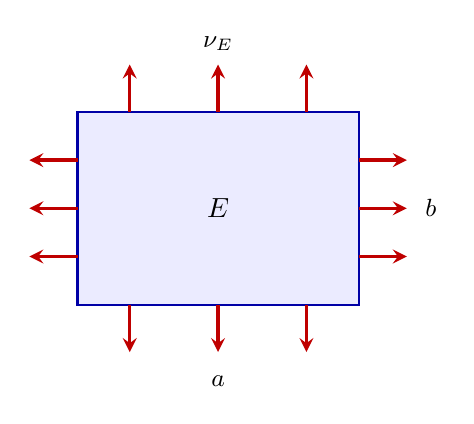
\begin{tikzpicture}[scale=1.02,>=stealth]
  \fill[blue!8] (0,0) rectangle (3.5,2.4);
  \draw[blue!65!black,thick] (0,0) rectangle (3.5,2.4);
  \node at (1.75,1.2) {$E$};
  \foreach \x in {0.65,1.75,2.85} {
    \draw[->,very thick,red!75!black] (\x,2.4)--(\x,2.99);
    \draw[->,very thick,red!75!black] (\x,0)--(\x,-0.59);
  }
  \foreach \y in {0.6,1.2,1.8} {
    \draw[->,very thick,red!75!black] (0,\y)--(-0.6,\y);
    \draw[->,very thick,red!75!black] (3.5,\y)--(4.1,\y);
  }
  \node[font=\small] at (1.75,3.25) {$\nu_E$};
  \node[font=\small] at (1.75,-.95) {$a$};
  \node[font=\small] at (4.4,1.2) {$b$};
\end{tikzpicture}
\end{center}
\noindent\emph{Rysunek:} miarowo-teoretyczna normalna i obwód
prostokąta w $\mathbb R^2$. Dla boków długości $a,b$
mamy $P(E;\mathbb R^2)=2(a+b)$ oraz
$D\chi_E=-\nu_E\mathcal H^1\llcorner\partial E$,
gdzie normalną na wierzchołkach można określić dowolnie:
cztery wierzchołki mają zerową $\mathcal H^1$-miarę
i nie wnoszą osobnej masy do obwodu.

\begin{lemat}[Pochodna i dopełnienie]
\label{lem:perimeter-complement-29}
Niech $E,F\subseteq\mathbb R^n$ będą mierzalne
w sensie Lebesgue'a, a $\Omega\subseteq\mathbb R^n$
będzie zbiorem otwartym. Wtedy
$D\chi_{E^c}=-D\chi_E$ jako dystrybucje na $\Omega$
oraz $P(E^c;\Omega)=P(E;\Omega)$.
Jeżeli $\lambda_n(E\triangle F)=0$,
to $P(E;\Omega)=P(F;\Omega)$.
\end{lemat}
\begin{proof}
Dla $\varphi\in C_c^1(\Omega;\mathbb R^n)$
przedłużenie przez zero jest klasy $C^1$ na całej
przestrzeni. Dla każdego $i$ całka z $\partial_i\varphi_i$
po $\mathbb R^n$ wynosi zero na mocy Fubiniego
i podstawowego twierdzenia rachunku całkowego,
bo całkowane funkcje mają zwarty nośnik.
Z tożsamości $\chi_{E^c}=1-\chi_E$ wynika więc
$\int_\Omega\chi_{E^c}\operatorname{div}\varphi
\,\mathrm d\lambda_n=-\int_\Omega\chi_E
\operatorname{div}\varphi\,\mathrm d\lambda_n$.
Daje to równość dystrybucji ze znakiem przeciwnym.
Ponieważ dopuszczalny test pozostaje dopuszczalny
po zmianie znaku, oba suprema są równe, także gdy
mają wartość $+\infty$.
Dla zbiorów równych prawie wszędzie ich funkcje
charakterystyczne są równe w $L^1_{\mathrm{loc}}$,
więc dają tę samą dystrybucję pochodnej.
\end{proof}

\section{Zwartość i półciągłość: dwa pełne dowody}
\begin{twierdzenie}[Dolna półciągłość obwodu]
\label{thm:perimeter-lsc-29}
Niech $\Omega\subseteq\mathbb R^n$ będzie zbiorem otwartym,
a $E,E_j\subseteq\mathbb R^n$, $j\ge1$, będą
mierzalne w sensie Lebesgue'a.
Jeśli $\chi_{E_j}\to\chi_E$ w
$L^1_{\mathrm{loc}}(\Omega)$, to
\[
 P(E;\Omega)\le\liminf_{j\to\infty}P(E_j;\Omega).
\]
Ogólniej, dla $u,u_j\in L^1_{\mathrm{loc}}(\Omega;\mathbb R)$,
jeśli $u_j\to u$ w $L^1_{\mathrm{loc}}(\Omega)$, to
$|Du|(\Omega)\le\liminf_j|Du_j|(\Omega)$.
\end{twierdzenie}
\begin{proof}
Ustalmy pole $\varphi\in C_c^1(\Omega;\mathbb R^n)$,
$|\varphi|\le1$. Niech $K=\operatorname{supp}\varphi\subseteq\Omega$.
Różnica całek testowych ma moduł nie większy
niż $\|\operatorname{div}\varphi\|_\infty
\int_K|u_j-u|\,\mathrm d\lambda_n$, a to dąży do zera
z lokalnej zbieżności w $L^1$.
Każda z całek po lewej jest nie większa niż
$|Du_j|(\Omega)$. Zatem całka dla $u$
jest nie większa niż $\liminf_j|Du_j|(\Omega)$.
Bierzemy supremum po wszystkich testach,
uzyskując tezę. Przypadek zbiorów otrzymujemy
po podstawieniu $u_j=\chi_{E_j}$.
\end{proof}

\begin{lemat}[Oszacowanie przesunięcia]
\label{lem:BV-translation-29}
Niech $n\ge1$ i $u\in BV(\mathbb R^n)$.
Wówczas dla każdego $h\in\mathbb R^n$
\[
 \int_{\mathbb R^n}|u(x+h)-u(x)|
 \,\mathrm d\lambda_n(x)\le|h|\,|Du|(\mathbb R^n).
\]
W szczególności dla mierzalnego zbioru $E$ o
skończonej mierze i skończonym obwodzie zachodzi
$\lambda_n((E+h)\triangle E)\le|h|P(E;\mathbb R^n)$.
\end{lemat}
\begin{proof}
Wybierzmy nieujemny gładki jądro wygładzające
$\rho\in C_c^\infty(B(0,1))$ z
$\int_{\mathbb R^n}\rho(x)\,\mathrm d\lambda_n(x)=1$ i
$\rho_\varepsilon(x)=\varepsilon^{-n}\rho(x/\varepsilon)$.
Niech $u_\varepsilon=u*\rho_\varepsilon$, czyli
$u_\varepsilon(x)=\int_{\mathbb R^n}u(y)
\rho_\varepsilon(x-y)\,\mathrm d\lambda_n(y)$.
Ponieważ $u\in L^1(\mathbb R^n)$, a wszystkie
pochodne $\rho_\varepsilon$ są ograniczone,
różniczkowanie pod całką jest uzasadnione
twierdzeniem o zbieżności zdominowanej
(stosowanym do ilorazów różnicowych).
W szczególności $u_\varepsilon$ jest gładka.
Dla ustalonego $x$ funkcja
$y\mapsto\rho_\varepsilon(x-y)$ jest testem gładkim
o zwartym nośniku. Z definicji pochodnej
dystrybucyjnej i Twierdzenia~\ref{thm:BV-measure-29}
otrzymujemy, dla $i=1,\ldots,n$,
\begin{align*}
 \partial_i u_\varepsilon(x)
 &=\int_{\mathbb R^n}u(y)
 \partial_{x_i}\rho_\varepsilon(x-y)\,\mathrm d\lambda_n(y)\\
 &=-\int_{\mathbb R^n}u(y)
 \partial_{y_i}\rho_\varepsilon(x-y)\,\mathrm d\lambda_n(y)\\
 &=\int_{\mathbb R^n}\rho_\varepsilon(x-y)\,\mathrm dD_i u(y).
\end{align*}
Stąd $\nabla u_\varepsilon=(Du)*\rho_\varepsilon$.
Jeżeli $Du=p|Du|$ jest rozkładem polarnym, to
$|p|=1$ prawie wszędzie względem $|Du|$.
Nieujemność jądra daje punktowo
\[
 |\nabla u_\varepsilon(x)|
 \le\int_{\mathbb R^n}\rho_\varepsilon(x-y)\,\mathrm d|Du|(y).
\]
Całkując względem $x$ i stosując Tonellego do
nieujemnej funkcji podcałkowej, otrzymujemy
\[
 \int_{\mathbb R^n}|\nabla u_\varepsilon|\,\mathrm d\lambda_n
 \le\int_{\mathbb R^n}
 \left(\int_{\mathbb R^n}\rho_\varepsilon(x-y)
 \,\mathrm d\lambda_n(x)\right)\mathrm d|Du|(y)
 =|Du|(\mathbb R^n).
\]
Podstawowe twierdzenie rachunku całkowego zastosowane
do funkcji $t\mapsto u_\varepsilon(x+th)$ daje
\[
 u_\varepsilon(x+h)-u_\varepsilon(x)
 =\int_0^1\nabla u_\varepsilon(x+th)\cdot h
 \,\mathrm d\lambda_1(t).
\]
Biorąc moduł, stosując nierówność Cauchy'ego--Schwarza,
Tonellego oraz niezmienniczość miary Lebesgue'a
względem translacji, otrzymujemy
\begin{align*}
 \int_{\mathbb R^n}|u_\varepsilon(x+h)-u_\varepsilon(x)|
 \,\mathrm d\lambda_n(x)
 &\le |h|\int_0^1\int_{\mathbb R^n}
 |\nabla u_\varepsilon(x+th)|\,\mathrm d\lambda_n(x)
 \,\mathrm d\lambda_1(t)\\
 &\le |h|\,|Du|(\mathbb R^n).
\end{align*}
Uzasadnijmy przejście do granicy.
Translacje są ciągłe w $L^1(\mathbb R^n)$: dla
funkcji ciągłych o zwartym nośniku wynika to
z jednostajnej ciągłości i wspólnego ograniczonego
nośnika przy małych przesunięciach; dla dowolnego
$u\in L^1$ korzystamy z gęstości tych funkcji
oraz z faktu, że translacja zachowuje normę $L^1$.
Z nierówności trójkąta i Tonellego wynika
\[
 \|u_\varepsilon-u\|_{L^1}
 \le\int_{\mathbb R^n}\rho(z)
 \|u(\,\cdot-\varepsilon z)-u\|_{L^1}\,\mathrm d\lambda_n(z)
 \longrightarrow0,
\]
gdzie stosujemy zbieżność zdominowaną z dominantą
$2\|u\|_{L^1}\rho(z)$.
Różnica między $u_\varepsilon(\cdot+h)-u_\varepsilon$
a $u(\cdot+h)-u$ ma normę nie większą niż
$2\|u_\varepsilon-u\|_{L^1}$. Przechodzimy zatem
do granicy po lewej stronie oszacowania, którego
prawa strona nie zależy od $\varepsilon$.

Dla $u=\chi_E$ założenia zapewniają $u\in BV$,
a $\chi_E(x+h)=\chi_{E-h}(x)$.
Norma różnicy jest więc równa
$\lambda_n((E-h)\triangle E)=
\lambda_n(E\triangle(E+h))$,
gdzie ostatnia równość wynika z translacji o $h$.
\end{proof}

\begin{twierdzenie}[Zwartość rodzin zbiorów o ograniczonym obwodzie]
\label{thm:perimeter-compact-29}
Niech $n\ge1$, $Q\subseteq\mathbb R^n$ będzie
ograniczonym prostopadłościanem, a $(E_j)_{j\ge1}$
ciągiem zbiorów mierzalnych w sensie Lebesgue'a
zawartych w $Q$ i spełniających
$\sup_j P(E_j;\mathbb R^n)<\infty$.
Wówczas istnieje podciąg $E_{j_\ell}$ oraz
mierzalny $E\subseteq\overline Q$, dla których
$\chi_{E_{j_\ell}}\to\chi_E$ w $L^1(\mathbb R^n)$,
a $P(E;\mathbb R^n)\le\liminf_\ell P(E_{j_\ell};\mathbb R^n)$.
\end{twierdzenie}
\begin{proof}
Niech $P_0=\sup_jP(E_j;\mathbb R^n)$.
Wybierzmy duży domknięty sześcian $S$, którego wnętrze
zawiera $\overline Q$. Dla $m\ge1$ podzielmy $S$
na $N_m=2^{mn}$ jednakowych kostek o boku
$\delta_m=2^{-m}\ell(S)$, gdzie $\ell(S)$ jest
długością boku $S$. Przyjmujemy kostki półotwarte,
pomijając zbiór miary zero na brzegu $S$.
Są one parami rozłączne i pokrywają $S$ prawie wszędzie.
Każdy $u_j=\chi_{E_j}$ należy do $BV(\mathbb R^n)$,
gdyż $\|u_j\|_{L^1}\le\lambda_n(Q)<\infty$ i
$|Du_j|(\mathbb R^n)\le P_0$. Zastępujemy go funkcją
$A_m u_j$, stałą na każdej kostce i równą
średniej $u_j$ na tej kostce, oraz równą $0$ poza $S$.
Współczynniki $A_m u_j$ należą do $[0,1]$.

Oszacujmy błąd przybliżenia. Dla kostki $C$
i jej średniej $u_C$ nierówność trójkąta i Fubini dają
\[
 \int_C|u_j(x)-u_C|\,\mathrm d\lambda_n(x)
 \le\frac1{\lambda_n(C)}\int_C\int_C
 |u_j(x)-u_j(y)|\,\mathrm d\lambda_n(y)
 \,\mathrm d\lambda_n(x).
\]
Dla każdej kostki podstawiamy $y=x+h$.
Dla ustalonego $h$ warunki $x,y\in C$ są równoważne
$x\in C\cap(C-h)$. Różnica dwóch punktów kostki
leży w $[-\delta_m,\delta_m]^n$. Wobec tego
\begin{align*}
 &\sum_C\int_C\int_C |u_j(x)-u_j(y)|
 \,\mathrm d\lambda_n(y)\,\mathrm d\lambda_n(x)\\
 &=\int_{[-\delta_m,\delta_m]^n}\sum_C
 \int_{C\cap(C-h)}|u_j(x+h)-u_j(x)|
 \,\mathrm d\lambda_n(x)\,\mathrm d\lambda_n(h).
\end{align*}
Zbiory $C\cap(C-h)$ są parami rozłączne dla
ustalonego $h$, ponieważ każdy z nich zawiera się
w odpowiedniej kostce $C$. Możemy więc zastąpić
sumę całek po nich jedną całką po $\mathbb R^n$
jako górnym oszacowaniem, bez dodatkowego czynnika
$N_m$. Ponieważ $\lambda_n(C)=\delta_m^n$,
otrzymujemy
\[
 \sum_C\int_C|u_j-u_C|\,\mathrm d\lambda_n
 \le\delta_m^{-n}\int_{[-\delta_m,\delta_m]^n}
 \int_{\mathbb R^n}|u_j(x+h)-u_j(x)|
 \,\mathrm d\lambda_n(x)\,\mathrm d\lambda_n(h)
 \le 2^n\sqrt n\,\delta_m P_0.
\]
Ostatnia nierówność wynika z Lematu
\ref{lem:BV-translation-29}, ponieważ $|h|\le\sqrt n\,\delta_m$
na całym $[-\delta_m,\delta_m]^n$, którego objętość
wynosi $(2\delta_m)^n$. Poza $S$ obie funkcje
są zerowe prawie wszędzie. Zatem
$\sup_j\|u_j-A_mu_j\|_{L^1}\le
2^n\sqrt n\,\delta_m P_0\to0$.

Dla ustalonego $m$ wektor średnich na kostkach
należy do zwartego sześcianu $[0,1]^{N_m}$.
Jeśli dwa wektory średnich mają współrzędne
$a_C,b_C$, to odpowiadające im funkcje schodkowe
różnią się w normie $L^1$ o
$\delta_m^n\sum_C|a_C-b_C|$. Zbieżność współrzędnych
daje zatem zbieżność w $L^1$.
Wybieramy dla $m=1$ podciąg indeksów, dla którego
$A_1u_j$ jest zbieżny, następnie jego podciąg dla
$m=2$ i tak dalej. Oznaczmy przez $j^{(m)}_\ell$
rosnący ciąg indeksów wybrany w $m$-tym kroku.
Kładziemy $j_\ell=j^{(\ell)}_\ell$. Indeksy
$j_\ell$ są ściśle rosnące, a dla każdego
ustalonego $m$ wszystkie $j_\ell$ przy $\ell\ge m$
należą do podciągu wybranego w kroku $m$.
Stąd $A_m u_{j_\ell}$ jest zbieżny w $L^1$.

Dla $\varepsilon>0$ wybieramy $m$ tak duże, aby
$\sup_j\|u_j-A_mu_j\|_{L^1}<\varepsilon/3$.
Dla dostatecznie dużych $\ell,r$ mamy także
$\|A_mu_{j_\ell}-A_mu_{j_r}\|_{L^1}<\varepsilon/3$.
Nierówność trójkąta daje
\[
 \|u_{j_\ell}-u_{j_r}\|_{L^1}
 \le\|u_{j_\ell}-A_mu_{j_\ell}\|_{L^1}
 +\|A_mu_{j_\ell}-A_mu_{j_r}\|_{L^1}
 +\|A_mu_{j_r}-u_{j_r}\|_{L^1}<\varepsilon.
\]
Z zupełności $L^1$ istnieje $u\in L^1(\mathbb R^n)$,
do którego ten podciąg zbiega w normie.

Wybieramy mierzalnego reprezentanta $u$.
Z faktu $u_{j_\ell}(x)\in\{0,1\}$ wynika
$\operatorname{dist}(u(x),\{0,1\})
\le|u(x)-u_{j_\ell}(x)|$.
Po scałkowaniu i przejściu do granicy otrzymujemy
$\int_{\mathbb R^n}\operatorname{dist}(u(x),\{0,1\})
\,\mathrm d\lambda_n(x)=0$.
Nieujemność funkcji podcałkowej daje
$u(x)\in\{0,1\}$ prawie wszędzie.
Ponadto
$\int_{\mathbb R^n\setminus\overline Q}|u|
\,\mathrm d\lambda_n\le\|u-u_{j_\ell}\|_{L^1}\to0$.
Definiujemy mierzalny zbiór
$E=\{x\in\overline Q:u(x)=1\}$, wówczas
$u=\chi_E$ prawie wszędzie. Nie musimy wybierać
dalszego podciągu. Zbieżność w $L^1(\mathbb R^n)$
implikuje zbieżność lokalną, więc
Twierdzenie~\ref{thm:perimeter-lsc-29} daje
$P(E;\mathbb R^n)\le\liminf_\ell P(E_{j_\ell};\mathbb R^n)
\le P_0$, co kończy dowód.
\end{proof}

\section{Normalna miarowo-teoretyczna i brzeg zredukowany}
\begin{definicja}[Normalna z pochodnej miary]
\label{def:normal-BV-29}
Niech $n\ge1$ i niech $E\subseteq\mathbb R^n$
będzie mierzalnym w sensie Lebesgue'a zbiorem
lokalnie skończonego obwodu.
Miara wektorowa $D\chi_E$ ma rozkład polarny
$D\chi_E=-\nu_E|D\chi_E|$, gdzie
$\nu_E:\mathbb R^n\to\mathbb R^n$ jest
$|D\chi_E|$-mierzalna i
$|\nu_E(x)|=1$ dla $|D\chi_E|$-prawie wszystkich $x$.
Funkcję $\nu_E$ nazywamy \emph{miarowo-teoretyczną
normalną zewnętrzną}. Jest ona wyznaczona jednoznacznie
z dokładnością do zbioru $|D\chi_E|$-miary zero.
\end{definicja}

\begin{proof}[Uzasadnienie istnienia normalnej]
Na każdej kuli $B(0,j)$, $j\ge1$, stosujemy
Twierdzenie~\ref{thm:BV-measure-29} do ograniczenia
$\chi_E$. Otrzymujemy rozkład
$D\chi_E=p_j|D\chi_E|$ na tej kuli, gdzie $p_j$
jest borelowskie i ma normę $1$ prawie wszędzie
względem wariacji. Na przecięciu dwóch kul
pola te są równe prawie wszędzie względem wariacji
z jednoznaczności pochodnych Radona--Nikodyma
każdej składowej. Definiujemy $p$ na rozłącznych
borelowskich warstwach $B(0,j)\setminus B(0,j-1)$
(przy $B(0,0)=\varnothing$) przez $p_j$.
Zgodność ograniczeń miar i przeliczalność warstw
dają $D\chi_E=p|D\chi_E|$ na każdym względnie
zwartym zbiorze borelowskim i $|p|=1$ prawie
wszędzie względem wariacji. Kładziemy $\nu_E=-p$.
Na ewentualnym zbiorze zerowym, gdzie norma pola
nie wynosi $1$, możemy przypisać wartość zero.
Jednoznaczność wynika z jednoznaczności gęstości
na każdej z kul, a przeliczalna suma zbiorów
wyjątkowych nadal ma miarę zero.
\end{proof}

\begin{definicja}[Punkty gęstości i brzeg miarowy]
Dla\label{def:measure-boundary-29} $n\ge1$ i zbioru mierzalnego w sensie
Lebesgue'a $E\subseteq\mathbb R^n$
niech $E^{(1)}$ i $E^{(0)}$ oznaczają zbiory punktów,
w których granica
\[
 \theta(E,x)=\lim_{r\downarrow0}
 \frac{\lambda_n(E\cap B(x,r))}{\lambda_n(B(x,r))}
\]
istnieje i wynosi odpowiednio $1$ lub $0$.
\emph{Brzegiem miarowym} nazywamy
$\partial^{\mathrm m}E=\mathbb R^n\setminus(E^{(0)}\cup E^{(1)})$.
Punkty, w których powyższa granica nie istnieje,
również należą do $\partial^{\mathrm m}E$.
\end{definicja}

\begin{lemat}[Brzeg miarowy jest objętościowo mały]
\label{lem:essential-boundary-null-29}
Dla każdego mierzalnego $E\subseteq\mathbb R^n$
zachodzi $\lambda_n(\partial^{\mathrm m}E)=0$.
\end{lemat}
\begin{proof}
Najpierw sprawdzamy borelowskość rozważanych zbiorów,
nawet jeśli sam $E$ nie jest borelowski.
Dla każdego $r>0$ funkcja
$f_r(x)=\lambda_n(E\cap B(x,r))/(\omega_n r^n)$,
gdzie $\omega_n=\lambda_n(B(0,1))$, jest ciągła:
moduł różnicy liczników w punktach $x,y$ nie
przekracza $\lambda_n(B(x,r)\triangle B(y,r))$,
która dąży do zera dla $y\to x$ (różnica kul
mieści się w pierścieniu o grubości dążącej do zera).
Dla $i\in\{0,1\}$ mamy
\[
 E^{(i)}=\bigcap_{l=1}^\infty\bigcup_{m=1}^\infty
 \bigcap_{\substack{q\in\mathbb Q\\0<q<1/m}}
 \{x:|f_q(x)-i|\le1/l\}.
\]
Równość wynika z ciągłości $r\mapsto f_r(x)$
dla $r>0$: przy zmianie promienia różnica objętości
kul dąży do zera. Zatem warunki dla wymiernych
promieni przenoszą się na wszystkie promienie
w tym samym przedziale. Prawa strona jest borelowska.
W konsekwencji także $\partial^{\mathrm m}E$
jest borelowski.
Twierdzenie~\ref{thm:lebesgue-diff-25} o różniczkowaniu
Lebesgue'a stosujemy do
$\chi_E\in L^1_{\mathrm{loc}}(\mathbb R^n)$.
Dla prawie każdego $x$ średnie funkcji $\chi_E$
na kulach $B(x,r)$ zbiegają do $\chi_E(x)$,
a więc do $0$ lub $1$. Takie punkty należą
do $E^{(0)}\cup E^{(1)}$. Ponadto
$\lambda_n(E\triangle E^{(1)})=0$.
Jeżeli $\lambda_n(E\triangle F)=0$, to dla każdej
kuli liczniki dla $E$ i $F$ są identyczne, więc
oba zbiory punktów gęstości i brzegi miarowe
pokrywają się punktowo.
\end{proof}

\begin{definicja}[Brzeg zredukowany]
\label{def:reduced-boundary-29}
Niech $n\ge1$ i niech $E\subseteq\mathbb R^n$
będzie mierzalnym zbiorem lokalnie skończonego obwodu.
\emph{Brzeg zredukowany} $\partial^*E$ składa się
z tych $x\in\mathbb R^n$, dla których
$|D\chi_E|(B(x,r))>0$ dla każdego $r>0$
oraz istnieje granica
\[
 \nu_E^*(x)=-\lim_{r\downarrow0}
 \frac{D\chi_E(B(x,r))}{|D\chi_E|(B(x,r))}
 \quad\text{o normie }1.
\]
To definicja punktowa, nie tylko klasy funkcji
wyznaczonej prawie wszędzie.
\end{definicja}

\begin{lemat}[Mierzalność brzegu zredukowanego i skupienie wariacji]
\label{lem:reduced-boundary-measurable-29}
Niech $E\subseteq\mathbb R^n$, $n\ge1$, będzie
mierzalnym zbiorem lokalnie skończonego obwodu
i niech $\mu=|D\chi_E|$.
Wówczas $\partial^*E$ jest borelowski,
$\mu(\mathbb R^n\setminus\partial^*E)=0$,
a $\nu_E^*$ jest borelowska na $\partial^*E$
i jest równa $\nu_E$ dla $\mu$-prawie wszystkich
punktów. Wyniki te nie wymagają twierdzenia
strukturalnego De Giorgiego.
\end{lemat}
\begin{proof}
Niech $S=\{x:\mu(B(x,r))>0\text{ dla każdego }r>0\}$.
Dopełnienie $S$ jest otwarte: jeśli $\mu(B(x,r))=0$,
to każdy punkt tej kuli ma mniejszą kulę
o mierze zero. Z drugiego aksjomatu przeliczalności
wynika, że dopełnienie $S$ można pokryć przeliczalnie
wieloma kulami miary zero, stąd $\mu(S^c)=0$.

Dla ustalonego $q>0$ funkcje
$x\mapsto\mu(B(x,q))$ oraz $x\mapsto D\chi_E(B(x,q))$
są borelowskie. Dla pierwszej stosujemy mierzalność
całki parametrycznej do borelowskiej funkcji
$(x,y)\mapsto\chi_{\{|x-y|<q\}}(x,y)$
względem $\sigma$-skończonej miary $\mu$.
Dla drugiej stosujemy tę samą własność do składowych
rozkładu polarnego, rozdzielając części dodatnie
i ujemne. Wszystkie całki po ograniczonej kuli są
skończone. Na $S$ definiujemy więc borelowskie pole
$w_q(x)=-D\chi_E(B(x,q))/\mu(B(x,q))$ o normie
nie większej niż $1$.
Dla każdego $x\in S$ i $r>0$, gdy $q_j\uparrow r$,
kule $B(x,q_j)$ rosną do $B(x,r)$.
Ciągłość miar od dołu (dla składowych ze znakiem
stosowana do obu części na ograniczonej kuli)
daje $w_{q_j}(x)\to w_r(x)$.
Zatem kryterium Cauchy'ego dla promieni wymiernych
wystarcza do istnienia granicy przy wszystkich
promieniach $r\downarrow0$.
Dokładniej, zbiór punktów $S$, dla których
granica istnieje, jest równy
\[
 S\cap\bigcap_{l=1}^\infty\bigcup_{m=1}^\infty
 \bigcap_{\substack{p,q\in\mathbb Q\\0<p,q<1/m}}
 \{x\in S:|w_p(x)-w_q(x)|\le1/l\}.
\]
Jest on borelowski. Na nim granica jest borelowska
jako granica ciągu pól $w_{1/j}$.
Warunek normy $1$ wybiera borelowski podzbiór
tego zbioru, dokładnie $\partial^*E$,
a granica jest tam równa $\nu_E^*$.

Na mocy Twierdzenia~\ref{thm:relative-lebesgue-25}
o różniczkowaniu całek względem miary Radona,
zastosowanego lokalnie do każdej składowej
ograniczonego pola $\nu_E$, dla $\mu$-prawie
każdego $x\in S$ zachodzi
\[
 \lim_{r\downarrow0}\frac{1}{\mu(B(x,r))}
 \int_{B(x,r)}\nu_E(y)\,\mathrm d\mu(y)=\nu_E(x).
\]
Lewa strona to właśnie granica $w_r(x)$.
Ponieważ $|\nu_E|=1$ prawie wszędzie względem
$\mu$, punkty te należą do $\partial^*E$
i zachodzi $\nu_E^*(x)=\nu_E(x)$.
Wraz z $\mu(S^c)=0$ daje to tezę.
\end{proof}

\begin{twierdzenie}[Twierdzenie Gaussa--Greena w postaci miarowej]
\label{thm:gauss-green-BV-29}
Niech $n\ge1$, $E\subseteq\mathbb R^n$ będzie
mierzalnym zbiorem lokalnie skończonego obwodu,
a $\varphi\in C_c^1(\mathbb R^n;\mathbb R^n)$.
Wtedy
\begin{equation}\label{eq:gauss-green-BV-29}
 \int_E\operatorname{div}\varphi(x)
 \,\mathrm d\lambda_n(x)
 =\int_{\mathbb R^n}\varphi(x)\cdot\nu_E(x)
 \,\mathrm d|D\chi_E|(x).
\end{equation}
\end{twierdzenie}
\begin{proof}
Definicja dystrybucyjnej pochodnej daje
$\int_E\operatorname{div}\varphi\,\mathrm d\lambda_n=-\int_{\mathbb R^n}\varphi\cdot\mathrm dD\chi_E$.
Podstawiamy rozkład polarny z
Definicji~\ref{def:normal-BV-29} i otrzymujemy
prawą stronę. Obie całki są skończone:
pierwsza ma ograniczoną funkcję podcałkową
o zwartym nośniku, druga jest ograniczona przez
$\|\varphi\|_\infty|D\chi_E|(\operatorname{supp}\varphi)$.
Z poprzedniego stwierdzenia można także zastąpić
prawą stronę całką po $\partial^*E$ względem
$|D\chi_E|$, z polem $\nu_E^*$ zamiast $\nu_E$.
Nie zastępujemy jednak jeszcze miary wariacji
miarą Hausdorffa: wymaga to dalszego twierdzenia
strukturalnego. Nie trzeba zakładać gładkości brzegu.
\end{proof}

\subsection*{Narzędzia do dowodu twierdzenia De Giorgiego}
Główny trud polega na wyprowadzeniu z samej miary $D\chi_E$
zarówno lokalnej płaskości brzegu, jak i jego miary powierzchniowej.
Przedstawimy ten argument w kilku krokach. W tej części zakładamy
$n\ge2$; przypadek $n=1$ omówimy na końcu dowodu.
Przez $\omega_j$ oznaczamy objętość kuli jednostkowej
w $\mathbb R^j$.

\begin{lemat}[Nierówności Sobolewa i względna nierówność izoperymetryczna]
\label{lem:dg-relative-isoperimetric}
Dla każdego $n\ge2$ istnieje $C_n>0$ taka, że
\begin{enumerate}[label=(\roman*)]
\item jeśli $v\in C_c^1(\mathbb R^n)$, to
 $\|v\|_{L^{n/(n-1)}(\mathbb R^n)}\le
 C_n\int_{\mathbb R^n}|\nabla v(x)|\,\mathrm d\lambda_n(x)$;
\item dla każdej kuli $B=B(x,r)$, $x\in\mathbb R^n$,
 $r>0$, i $v\in BV(B)$ zachodzi
 $\|v-v_B\|_{L^{n/(n-1)}(B)}\le C_n|Dv|(B)$,
 gdzie $v_B=\lambda_n(B)^{-1}\int_Bv\,\mathrm d\lambda_n$;
\item dla mierzalnego $E$ o lokalnie skończonym obwodzie
 i dowolnej kuli $B=B(x,r)$ zachodzi
 \[
 \min\{\lambda_n(E\cap B),\lambda_n(B\setminus E)\}^{(n-1)/n}
 \le C_n P(E;B).
 \]
 Ponadto, jeżeli $A\subset\mathbb R^n$ jest mierzalny,
 ma skończoną miarę i skończony obwód, to
 $\lambda_n(A)^{(n-1)/n}\le C_nP(A;\mathbb R^n)$.
\end{enumerate}
\end{lemat}
\begin{proof}
Dla nieujemnych mierzalnych funkcji
$g_i\in L^1(\mathbb R^{n-1})$, $i=1,\ldots,n$,
oznaczamy przez $x_{\widehat i}$ wektor otrzymany
przez usunięcie $i$-tej współrzędnej z $x$.
Zachodzi nierówność
\[
 \int_{\mathbb R^n}\prod_{i=1}^n
 g_i(x_{\widehat i})^{1/(n-1)}\,\mathrm d\lambda_n(x)
 \le\prod_{i=1}^n
 \left(\int_{\mathbb R^{n-1}}g_i(y)\,
 \mathrm d\lambda_{n-1}(y)\right)^{1/(n-1)}.
\]
Oznaczmy lewą stronę przez $I$.
Dla $n=2$ nierówność jest równością Tonellego.
W kroku indukcyjnym, przy $n\ge3$, oznaczamy
$h_i(x'_{\widehat i})=\int_{\mathbb R}
 g_i(x_{\widehat i})\,\mathrm d\lambda_1(x_n)$
przy $i<n$, gdzie $x'=(x_1,\ldots,x_{n-1})$.
Z twierdzenia Tonellego funkcje $h_i$ są mierzalne
i całkowalne, z całkami równymi całkom $g_i$.
Nierówność Höldera dla $n-1$ czynników z jednakowymi
wykładnikami $n-1$ przy całkowaniu po $x_n$ daje
\[
 I\le\int_{\mathbb R^{n-1}}g_n(x')^{1/(n-1)}
 \prod_{i<n}h_i(x'_{\widehat i})^{1/(n-1)}
 \,\mathrm d\lambda_{n-1}(x').
\]
Stosując ponownie Höldera, z wykładnikami
$n-1$ oraz $(n-1)/(n-2)$, a następnie
założenie indukcyjne dla $(n-1)$ funkcji $h_i$,
otrzymujemy następujący rachunek. Oznaczmy
$G_i=\int_{\mathbb R^{n-1}}g_i(y)\,
\mathrm d\lambda_{n-1}(y)$ oraz
\[
 K=\int_{\mathbb R^{n-1}}\prod_{i<n}
 h_i(x'_{\widehat i})^{1/(n-2)}
 \,\mathrm d\lambda_{n-1}(x').
\]
Wtedy
\[
 I\le G_n^{1/(n-1)}K^{(n-2)/(n-1)}
 \le\prod_{i=1}^n G_i^{1/(n-1)}.
\]
To zamyka indukcję.
Dla $v\in C_c^1$ kładziemy
$g_i(x_{\widehat i})=\int_{\mathbb R}
|\partial_i v(x)|\,\mathrm d\lambda_1(x_i)$.
Z zasadniczego twierdzenia rachunku całkowego wynika
$|v(x)|\le g_i(x_{\widehat i})$ dla każdego $i$.
Mnożymy te nierówności i podnosimy do potęgi
$1/(n-1)$, otrzymując
$|v|^{n/(n-1)}\le\prod_i g_i^{1/(n-1)}$.
Całkujemy i stosujemy poprzednie oszacowanie,
a następnie podnosimy obie strony do potęgi
$(n-1)/n$. Wobec $\int g_i=\|\partial_i v\|_1$
oraz $|\partial_i v|\le|\nabla v|$ mamy
$\|v\|_{n/(n-1)}\le\prod_i\|\partial_i v\|_1^{1/n}
\le\|\nabla v\|_1$. To dowodzi (i).

Dla (ii) najpierw rozważamy funkcje klasy $C^1$
na otoczeniu domknięcia kuli jednostkowej $B=B(0,1)$.
Z definicji średniej i nierówności trójkąta
\[
 \|v-v_B\|_{L^1(B)}
 \le\lambda_n(B)^{-1}\int_B\int_B|v(x)-v(y)|
 \,\mathrm d\lambda_n(x)\,\mathrm d\lambda_n(y).
\]
Wypukłość kuli i podstawowe twierdzenie rachunku
całkowego na odcinku dają
$|v(x)-v(y)|\le2\int_0^1
|\nabla v((1-t)x+ty)|\,\mathrm d\lambda_1(t)$.
Dla ustalonego $y$ i $0\le t\le1/2$ odwzorowanie
$x\mapsto(1-t)x+ty$ ma wyznacznik $(1-t)^n$,
a obraz $B$ zawiera się w $B$. Stąd
\[
 \int_B|\nabla v((1-t)x+ty)|\,\mathrm d\lambda_n(x)
 \le2^n\int_B|\nabla v(z)|\,\mathrm d\lambda_n(z).
\]
Dla $1/2\le t\le1$ otrzymujemy to samo oszacowanie
całki po $y$ przy ustalonym $x$ przez zmianę
$y\mapsto(1-t)x+ty$ o wyznaczniku $t^n$.
Tonelli, całkowanie po pozostałej zmiennej oraz
po $t$ dają
$\|v-v_B\|_{L^1(B)}\le2^{n+1}\|\nabla v\|_{L^1(B)}$.

Aby podnieść wykładnik, kładziemy $w=v-v_B$
oraz definiujemy funkcję $\widetilde w$ równą $w$
na domkniętej kuli jednostkowej, a na pierścieniu
$1<|x|<3/2$ równą $w(R(x))$, gdzie
$R(x)=(2-|x|)x/|x|$. Odwzorowanie $R$ jest
dyfeomorfizmem pierścienia na $\{1/2<|y|<1\}$.
Różniczka w kierunku radialnym ma wartość własną
$-1$, a w kierunkach stycznych $(2-|x|)/|x|$,
zawartą w przedziale $(1/3,1)$. W szczególności
$\|DR\|\le1$ oraz $|\det DR|\ge3^{-(n-1)}$.
Wybieramy $\theta\in C_c^\infty(B(0,3/2))$
o wartościach w $[0,1]$, równą $1$ na $\overline B$,
i definiujemy $V=\theta\widetilde w$, przedłużając
przez zero poza kulę o promieniu $3/2$.
Funkcja $V$ jest ciągła, ma zwarty nośnik,
a w obu częściach oddzielonych sferą jednostkową
jest klasy $C^1$ z ograniczonymi pochodnymi.
Jej pochodne dystrybucyjne są równe klasycznym
pochodnym na obu częściach: całkując przez części
w kuli i w pierścieniu (twierdzenie o dywergencji
dla brzegu klasy $C^1$), widzimy, że wyrazy brzegowe
na wspólnej sferze znoszą się, ponieważ wartości
$V$ są tam zgodne, a normalne przeciwne.
Przy zewnętrznym brzegu $V$ znika.
Można też zastosować ten argument do pierścieni
odległych od sfery o $\delta>0$ i przejść
$\delta\downarrow0$, korzystając z ciągłości
i ograniczoności funkcji oraz pochodnych.
Wobec tego $DV=\nabla V\,\lambda_n$, gdzie
gradient jest określony kawałkami, a sfera
ma zerową miarę Lebesgue'a.
Reguła iloczynu i zamiana zmiennych przez $R$
na pierścieniu dają
\[
 \|\nabla V\|_{L^1(\mathbb R^n)}
 \le C_n\bigl(\|\nabla v\|_{L^1(B)}+\|w\|_{L^1(B)}\bigr)
 \le C_n\|\nabla v\|_{L^1(B)}.
\]
Stała zależy tylko od wymiaru i ustalonej funkcji
odcinającej, nie od $v$.
Wygładzenia $V_\varepsilon=V*\rho_\varepsilon$
są gładkie i mają zwarty nośnik; według rachunku
splotów z dowodu Lematu~\ref{lem:BV-translation-29}
$\|\nabla V_\varepsilon\|_1\le\|\nabla V\|_1$,
a $V_\varepsilon\to V$ w $L^1$.
Wybieramy podciąg zbieżny prawie wszędzie.
Z (i) i lematu Fatou dla potęgi $p=n/(n-1)$
wynika $\|V\|_{L^p}\le C_n\|\nabla V\|_{L^1}$.
Ponieważ $V=w$ na $B$, otrzymujemy (ii) dla
funkcji klasy $C^1$ na otoczeniu $\overline B$.

Dla dowolnej kuli $B(x,r)$ stosujemy ten wynik
do funkcji $z\mapsto v(x+rz)$ na kuli jednostkowej.
Jej średnia jest równa $v_{B(x,r)}$. Norma $L^p$
skaluje się przez czynnik $r^{-n/p}=r^{1-n}$,
a norma $L^1$ gradientu przez $r^{1-n}$, co
dowodzi nierówności z tą samą stałą na każdej kuli. Dla $v\in BV(B(x,r))$ ustalamy $0<s<r$.
Wybieramy nieujemne jądro $\rho_\varepsilon$
o całce $1$ i nośniku w $B(0,\varepsilon)$,
gdzie $\varepsilon<r-s$. Funkcję $v$ możemy
przedłużyć przez zero jako funkcję $L^1$,
ale nie zakładamy, że przedłużenie należy do $BV$.
Dla $z\in B(x,s)$ test
$y\mapsto\rho_\varepsilon(z-y)$ ma zwarty
nośnik w $B(x,r)$, dlatego tożsamość splotu
z pochodną miarową zachodzi w tej kuli.
Rozkład polarny i Tonelli dają
\[
 \int_{B(x,s)}|\nabla v_\varepsilon(z)|\,\mathrm d\lambda_n(z)
 \le |Dv|(B(x,s+\varepsilon))
 \le |Dv|(B(x,r)).
\]
W pierwszej nierówności wykorzystujemy, że jądro
jest zerowe dla $|z-y|\ge\varepsilon$, a całka
jądra po $z\in B(x,s)$ nie przekracza $1$.
Funkcja $v_\varepsilon$ jest gładka na otoczeniu
domknięcia $B(x,s)$, więc stosujemy udowodnioną
nierówność na tej kuli. Zbieżność splotu w $L^1$
daje $v_\varepsilon\to v$ w $L^1(B(x,s))$,
a w szczególności średnie
$(v_\varepsilon)_{B(x,s)}\to v_{B(x,s)}$.
Wybierając podciąg zbieżny prawie wszędzie i
stosując lemat Fatou do potęgi $p$, uzyskujemy
\[
 \|v-v_{B(x,s)}\|_{L^p(B(x,s))}
 \le C_n|Dv|(B(x,r)).
\]
Nie potrzebujemy zakładać, że sfera o promieniu
$s$ ma zerową miarę wariacji.
Teraz wybieramy $s_j\uparrow r$.
Ponieważ $v\in L^1(B(x,r))$ i
$\lambda_n(B(x,s_j))\to\lambda_n(B(x,r))$,
średnie $v_{B(x,s_j)}$ zbiegają do $v_{B(x,r)}$.
Funkcje
$\chi_{B(x,s_j)}|v-v_{B(x,s_j)}|^p$ zbiegają
punktowo prawie wszędzie w $B(x,r)$ do
$|v-v_{B(x,r)}|^p$. Ponowne zastosowanie lematu
Fatou daje (ii) z prawą stroną
$C_n|Dv|(B(x,r))$, bez żadnego składnika brzegowego.

W (iii) bierzemy $v=\chi_E$, a w (ii)
$v_B=\theta:=\lambda_n(E\cap B)/\lambda_n(B)$.
Jeśli $\theta\le1/2$, to $|\chi_E-\theta|\ge1/2$
na $E\cap B$, a jeżeli $\theta\ge1/2$, to
$|\chi_E-\theta|\ge1/2$ na $B\setminus E$.
W obu przypadkach
\[
 \|\chi_E-\theta\|_{L^p(B)}
 \ge\frac12\min\{\lambda_n(E\cap B),
                   \lambda_n(B\setminus E)\}^{1/p}.
\]
Po zastosowaniu (ii) i powiększeniu stałej
otrzymujemy względną nierówność izoperymetryczną.

Dla ostatniej nierówności nie możemy bezpośrednio
stosować (i) do wygładzenia $\chi_A$, ponieważ
$A$ nie musi być ograniczony. Niech
$w_\varepsilon=\chi_A*\rho_\varepsilon$.
Z Lematu~\ref{lem:BV-translation-29} i jego dowodu
mamy $\|w_\varepsilon\|_1\le\lambda_n(A)$,
$\|\nabla w_\varepsilon\|_1\le P(A;\mathbb R^n)$
oraz zbieżność $w_\varepsilon\to\chi_A$ w $L^1$.
Wybieramy $\zeta\in C_c^\infty(B(0,2))$
równą $1$ na $B(0,1)$, o wartościach w $[0,1]$,
i kładziemy $\zeta_R(x)=\zeta(x/R)$.
Wówczas $\zeta_R w_\varepsilon\in C_c^1$,
a z (i) i reguły iloczynu wynika
\[
 \|\zeta_R w_\varepsilon\|_{L^p}
 \le C_n\left(P(A;\mathbb R^n)
 +R^{-1}\|\nabla\zeta\|_\infty\lambda_n(A)\right).
\]
Najpierw $R\to\infty$; lemat Fatou daje
$\|w_\varepsilon\|_{L^p}\le C_nP(A;\mathbb R^n)$.
Następnie wybieramy $\varepsilon_j\downarrow0$
z $w_{\varepsilon_j}\to\chi_A$ prawie wszędzie,
co jest możliwe dzięki zbieżności w $L^1$.
Jeszcze raz stosując lemat Fatou, otrzymujemy
$\lambda_n(A)^{1/p}=\|\chi_A\|_{L^p}
\le C_nP(A;\mathbb R^n)$, zgodnie z tezą.
\end{proof}

\begin{lemat}[Przecięcie zbioru skończonego obwodu z kulą]
\label{lem:dg-ball-cut}
Niech $n\ge2$, $E\subseteq\mathbb R^n$ będzie
mierzalnym w sensie Lebesgue'a zbiorem lokalnie
skończonego obwodu, $x\in\mathbb R^n$ oraz
$\mu=|D\chi_E|$. Dla $\lambda_1$-prawie wszystkich
$r>0$ zbiór $E\cap B(x,r)$ ma skończony obwód
globalny i zachodzi równość skończonych miar wektorowych
\[
 D\chi_{E\cap B(x,r)}
 =\chi_{B(x,r)}D\chi_E
 -\frac{y-x}{r}\,\chi_E(y)
 \mathcal H^{n-1}\llcorner\partial B(x,r).
\]
W ostatnim członie możemy użyć dowolnego
borelowskiego reprezentanta $\chi_E$ (dwa takie
reprezentanty zgadzają się $\mathcal H^{n-1}$-prawie
wszędzie na sferach dla prawie wszystkich promieni).
Ponadto funkcje $v(r)=\lambda_n(E\cap B(x,r))$
oraz $w(r)=\lambda_n(B(x,r)\setminus E)$ są
lokalnie bezwzględnie ciągłe na $[0,\infty)$
i spełniają
\[
 v'(r)=\mathcal H^{n-1}(E\cap\partial B(x,r)),\qquad
 w'(r)=\mathcal H^{n-1}(E^c\cap\partial B(x,r))
\]
dla prawie wszystkich $r>0$.
\end{lemat}
\begin{proof}
Wybieramy borelowski zbiór różniący się od $E$
o zbiór miary Lebesgue'a zero i zastępujemy nim
$E$ w rachunku. Nie zmienia to pochodnej
dystrybucyjnej ani funkcji $v,w$.
Dla nieujemnej funkcji borelowskiej $f$ obowiązuje
polarny wzór całkowy
\[
 \int_{\mathbb R^n} f(y)\,\mathrm d\lambda_n(y)
 =\int_0^\infty\int_{\partial B(x,t)} f(y)
 \,\mathrm d\mathcal H^{n-1}(y)\,\mathrm d\lambda_1(t).
\]
Jest to wzór koobszaru z Rozdziału~\ref{ch:area-coarea-28}
dla funkcji $y\mapsto|y-x|$, której gradient ma normę
$1$ poza singletonem $\{x\}$.
Zastosowanie go do funkcji charakterystycznej
różnicy symetrycznej dwóch borelowskich reprezentantów
pokazuje ich zgodność prawie wszędzie na sferach
dla prawie wszystkich promieni. W dalszym rachunku
ustalamy jeden reprezentant.

Wybieramy nieujemną $\kappa\in C_c^\infty((0,1))$
o całce $1$ i definiujemy
$\eta(s)=\int_s^\infty\kappa(t)\,\mathrm d\lambda_1(t)$.
Wtedy $\eta=1$ na $(-\infty,0]$, $\eta=0$
na $[1,\infty)$ oraz $\eta'=-\kappa$.
Dla $r>0$ i $\varepsilon>0$ kładziemy
$\zeta_\varepsilon(y)=\eta((|y-x|-r)/\varepsilon)$.
Funkcja jest gładka także w otoczeniu $x$,
gdyż tam jest stała, i ma zwarty nośnik.
Dla każdego pola $\varphi\in C_c^1(\mathbb R^n;\mathbb R^n)$
reguła iloczynu dla dywergencji daje bezpośrednio
\begin{align*}
 -\int \chi_E\zeta_\varepsilon\operatorname{div}\varphi
 \,\mathrm d\lambda_n
 &=-\int\chi_E\operatorname{div}(\zeta_\varepsilon\varphi)
 \,\mathrm d\lambda_n
 +\int\chi_E\varphi\cdot\nabla\zeta_\varepsilon
 \,\mathrm d\lambda_n\\
 &=\int\zeta_\varepsilon\varphi\cdot\mathrm dD\chi_E
 +\int\chi_E\varphi\cdot\nabla\zeta_\varepsilon
 \,\mathrm d\lambda_n.
\end{align*}
Wszystkie całki bez jawnej dziedziny w tym rachunku
są po $\mathbb R^n$.
Nie trzeba wygładzać $\chi_E$ ani zakładać
zbieżności jej wygładzonych pochodnych.
Po lewej stronie zbieżność zdominowana daje
granicę $-\int_{E\cap B(x,r)}\operatorname{div}\varphi
\,\mathrm d\lambda_n$, ponieważ sfera ma zerową
miarę Lebesgue'a.

Zbiór promieni $r>0$, dla których
$\mu(\partial B(x,r))>0$, jest co najwyżej
przeliczalny. Istotnie, na każdej kuli domkniętej
$\overline B(x,M)$ miara $\mu$ jest skończona,
a sfery są rozłączne. Dla $r\le M$ tylko skończenie
wiele sfer może mieć masę co najmniej $1/k$,
dla ustalonego $k\ge1$. Sumujemy po $M,k\in\mathbb N$.
Dla pozostałych promieni pierwszy składnik po
prawej stronie zbiega do
$\int_{B(x,r)}\varphi\cdot\mathrm dD\chi_E$,
na mocy zbieżności zdominowanej względem
lokalnie skończonej wariacji $\mu$.

Dla drugiego składnika definiujemy funkcję
\[
 F_\varphi(t)=\int_{\partial B(x,t)}
 \chi_E(y)\varphi(y)\cdot\frac{y-x}{t}
 \,\mathrm d\mathcal H^{n-1}(y),\qquad t>0.
\]
Jest ona mierzalna, co widać po parametryzacji
sfer przez $y=x+t\theta$, $\theta\in\partial B(0,1)$,
ze skalowaniem miary powierzchniowej przez $t^{n-1}$,
i zastosowaniu Fubiniego. Ponadto
$|F_\varphi(t)|\le\|\varphi\|_\infty n\omega_n t^{n-1}$.
Zatem $F_\varphi$ jest lokalnie całkowalna.
Ze wzoru na gradient $\zeta_\varepsilon$ oraz
polarnego wzoru całkowego otrzymujemy
\[
 \int\chi_E\varphi\cdot\nabla\zeta_\varepsilon
 \,\mathrm d\lambda_n
 =-\int_r^{r+\varepsilon}
 \frac1\varepsilon\kappa((t-r)/\varepsilon)
 F_\varphi(t)\,\mathrm d\lambda_1(t).
\]
Dla każdego punktu Lebesgue'a $r>0$ funkcji
$F_\varphi$ różnica między prawą stroną a
$-F_\varphi(r)$ ma moduł nie większy niż
\[
 \frac{\|\kappa\|_\infty}{\varepsilon}
 \int_r^{r+\varepsilon}|F_\varphi(t)-F_\varphi(r)|
 \,\mathrm d\lambda_1(t)\longrightarrow0.
\]
Zbieżność wynika z twierdzenia o różniczkowaniu
Lebesgue'a w wymiarze jeden (średnią jednostronną
ograniczamy przez dwukrotność średniej symetrycznej).

Aby zbiór dobrych promieni nie zależał od wyboru
pola testowego, wybieramy przeliczalną rodzinę
$\mathcal T\subset C_c^1(\mathbb R^n;\mathbb R^n)$
taką, że każde pole testowe można przybliżyć
w normie $C^1$ przez pola z $\mathcal T$,
o nośnikach we wspólnej kuli.
Istnienie takiej rodziny wynika następująco.
Dla każdego całkowitego $M\ge1$ przestrzeń pól
$C_c^1$ o nośniku w $\overline B(0,M)$
z normą $C^1$ zanurza się izometrycznie
(przy normie sumy norm supremum) w skończony
produkt przestrzeni $C(\overline B(0,M))$,
przypisując polu jego składowe oraz ich pierwsze
pochodne. Przestrzeń $C$ na zwartym podzbiorze
euklidesowym jest ośrodkowa, np. dzięki jednostajnej
aproksymacji wielomianami o współczynnikach wymiernych.
Podprzestrzeń przestrzeni metrycznej ośrodkowej
jest ośrodkowa. Wybieramy więc przeliczalny
gęsty podzbiór dla każdego $M$ i bierzemy ich sumę.
Usuwamy z $(0,\infty)$ przeliczalny zbiór promieni
o dodatniej masie sfery oraz zbiory punktów,
które nie są punktami Lebesgue'a $F_\varphi$,
dla wszystkich $\varphi\in\mathcal T$.
Pozostaje zbiór pełnej miary.

Dla każdego promienia z tego zbioru otrzymana
tożsamość zachodzi jednocześnie dla wszystkich
$\varphi\in\mathcal T$. Przenosimy ją na dowolne
pole testowe przez aproksymację w normie $C^1$.
Lewa strona jest ciągła w tej normie, z oszacowaniem
przez $\lambda_n(B(x,r))$ razy normę supremum
dywergencji; obie całki miarowe są ciągłe nawet
w normie supremum, z oszacowaniami odpowiednio
przez $\mu(B(x,r))$ i $n\omega_n r^{n-1}$.
W konsekwencji pochodną dystrybucyjną
$\chi_{E\cap B(x,r)}$ reprezentuje skończona
miara wektorowa podana w tezie. Tożsamość testowa
daje skończoność wariacji, więc twierdzenie o
reprezentacji i jego jednoznaczność identyfikują
tę miarę z $D\chi_{E\cap B(x,r)}$.

Na koniec polarny wzór całkowy daje dla każdego $r>0$
\[
 v(r)=\int_0^r\mathcal H^{n-1}(E\cap\partial B(x,t))
 \,\mathrm d\lambda_1(t)
\]
i analogiczny wzór dla $w$, z $E^c$ zamiast $E$.
Funkcje podcałkowe są mierzalne i ograniczone przez
$n\omega_n t^{n-1}$, zatem są całkowalne na każdym
ograniczonym przedziale. Podstawowe twierdzenie
rachunku całkowego dla całki Lebesgue'a daje
lokalną bezwzględną ciągłość i podane wzory
na pochodne dla prawie wszystkich $r>0$.
Przecinając z wcześniejszym zbiorem pełnej miary,
otrzymujemy wszystkie te tożsamości jednocześnie.
\end{proof}

\begin{lemat}[Oszacowania gęstości na brzegu zredukowanym]
\label{lem:dg-density}
Niech $n\ge2$, $E\subseteq\mathbb R^n$ będzie
mierzalnym zbiorem lokalnie skończonego obwodu,
$\mu=|D\chi_E|$, a $x\in\partial^*E$.
Istnieją liczby $r_x>0$ i $0<c_n<C_n<\infty$,
zależne wyłącznie od wymiaru poza $r_x$, takie że
\[
 c_nr^{n-1}\le\mu(B(x,r))\le C_nr^{n-1},\qquad
 \lambda_n(E\cap B(x,r))\ge c_nr^n,\quad
 \lambda_n(E^c\cap B(x,r))\ge c_nr^n
\]
dla każdego $0<r<r_x$.
\end{lemat}
\begin{proof}
Niech $\nu_0=\nu_E^*(x)$ oraz
$D\chi_E=-\nu_E\mu$. Z definicji brzegu
zredukowanego otrzymujemy
\[
 \frac{1}{\mu(B(x,r))}\int_{B(x,r)}\nu_E(y)
 \,\mathrm d\mu(y)\longrightarrow\nu_0.
\]
Ponieważ $|\nu_E|=|\nu_0|=1$,
\[
 \frac1{\mu(B(x,r))}\int_{B(x,r)}
 |\nu_E(y)-\nu_0|^2\,\mathrm d\mu(y)
 =2-2\nu_0\cdot\frac{\int_{B(x,r)}\nu_E(y)\,\mathrm d\mu(y)}
 {\mu(B(x,r))}\longrightarrow0.
\]
W szczególności, dla małych $r$ mamy
$\int_{B(x,r)}\nu_0\cdot\nu_E(y)\,\mathrm d\mu(y)
\ge\frac12\mu(B(x,r))$.

Ustalmy $r_x>0$ tak, aby oszacowanie z czynnikiem
$1/2$ zachodziło dla wszystkich $0<r<r_x$.
Przez $v,w$ oznaczamy funkcje objętości z
Lematu~\ref{lem:dg-ball-cut}.
Dla promieni dobrych w tym lemacie zarówno dla
$E$, jak i dla $E^c$ mamy skończone miary pochodnych
obu przecięć, o nośniku w $\overline B(x,r)$.
Ich całkowite masy wektorowe są zerowe:
dla dowolnego stałego wektora $e$ wybieramy
$\theta\in C_c^\infty(\mathbb R^n)$ równą $1$
na otoczeniu $\overline B(x,r)$.
W tożsamości testowej dla pola $\theta e$
dywergencja znika na obu przecięciach,
a całka względem miary pochodnej jest równa
iloczynowi skalarnemu $e$ z jej masą wektorową.
Z dowolności $e$ wynika zerowanie masy.

Wobec $D\chi_E=-\nu_E\mu$ wzór przecięcia daje
\[
 \int_{B(x,r)}\nu_E\,\mathrm d\mu
 =-\int_{\partial B(x,r)}\chi_E(y)\frac{y-x}{r}
 \,\mathrm d\mathcal H^{n-1}(y).
\]
Iloczyn skalarny z $\nu_0$, a następnie
$|\nu_0\cdot(y-x)/r|\le1$, dają
$\mu(B(x,r))/2\le v'(r)$ dla prawie wszystkich
$r\in(0,r_x)$. Analogicznie, ponieważ
$D\chi_{E^c}=-D\chi_E$, normalna dla dopełnienia
jest przeciwna, a w analogicznym oszacowaniu
używamy $-\nu_0$. Otrzymujemy
$\mu(B(x,r))/2\le w'(r)$ na wspólnym zbiorze
promieni pełnej miary.
Ponieważ $v'(r),w'(r)\le n\omega_n r^{n-1}$,
mamy $\mu(B(x,r))\le2n\omega_n r^{n-1}$
dla prawie wszystkich małych $r$.
Dla dowolnego $r\in(0,r_x)$ wybieramy ciąg
dobrych promieni $r_j\downarrow r$ z $r_j<r_x$.
Monotoniczność $\mu(B(x,r))\le\mu(B(x,r_j))$
i przejście do granicy w oszacowaniu liczbowym
dają tę samą nierówność dla każdego takiego $r$.

Dla dobrego promienia miara pochodnej przecięcia
jest sumą miary ograniczonej do otwartej kuli
i miary powierzchniowej na sferze. Z nierówności
trójkąta dla wariacji wynika
$P(E\cap B(x,r);\mathbb R^n)\le
\mu(B(x,r))+v'(r)$. Objętość przecięcia jest
skończona, więc globalna nierówność izoperymetryczna
z Lematu~\ref{lem:dg-relative-isoperimetric} daje
\[
 v(r)^{(n-1)/n}\le C_n
 \bigl(\mu(B(x,r))+v'(r)\bigr)
 \le C'_n v'(r).
\]
Analogicznie $w(r)^{(n-1)/n}\le C'_nw'(r)$
dla prawie wszystkich $r\in(0,r_x)$.
Z warunku $\mu(B(x,r))>0$ wynika, że
$v(r),w(r)>0$ dla każdego $r>0$.
W przeciwnym razie $\chi_E$ byłaby równa prawie
wszędzie odpowiednio $0$ lub $1$ w tej kuli.
Całka z dywergencji każdego pola testowego
o nośniku w kuli byłaby wtedy zerowa,
a z definicji wariacji i tożsamości na otwartych
zbiorach wynikałoby $\mu(B(x,r))=0$.

Ustalmy $0<\varepsilon<r<r_x$.
Funkcja $v$ jest bezwzględnie ciągła i niemalejąca,
a $v(\varepsilon)>0$. Na przedziale
$[\varepsilon,r]$ funkcja $v^{1/n}$ jest
bezwzględnie ciągła, gdyż składamy $v$ z funkcją
klasy $C^1$ o ograniczonej pochodnej na
$[v(\varepsilon),v(r)]$. Reguła łańcuchowa dla
funkcji bezwzględnie ciągłych daje
\[
 (v^{1/n})'(t)=\frac1n
 v(t)^{-(n-1)/n}v'(t)\ge\frac1{nC'_n}
\]
dla prawie wszystkich $t\in(\varepsilon,r)$.
Całkowanie daje
$v(r)^{1/n}\ge v(\varepsilon)^{1/n}+
(r-\varepsilon)/(nC'_n)$. Ponieważ
$0\le v(\varepsilon)\le\omega_n\varepsilon^n$,
przejście $\varepsilon\downarrow0$ daje
$v(r)\ge(r/(nC'_n))^n$. Identyczny rachunek
dla $w$ daje $w(r)\ge(r/(nC'_n))^n$.
Obie nierówności zachodzą dla każdego
$r\in(0,r_x)$, mimo że nierówności różniczkowe
zachodziły jedynie prawie wszędzie.
Względna nierówność izoperymetryczna z
Lematu~\ref{lem:dg-relative-isoperimetric}
daje teraz $\mu(B(x,r))\ge c_nr^{n-1}$.
\end{proof}

\begin{lemat}[Półprzestrzeń jako jedyna granica po przeskalowaniu]
\label{lem:dg-blowup}
Niech $n\ge2$, $E\subseteq\mathbb R^n$ będzie
mierzalnym zbiorem lokalnie skończonego obwodu,
$\mu=|D\chi_E|$, $x\in\partial^*E$,
$\nu=\nu_E^*(x)$ oraz, dla $r>0$,
$E_{x,r}=\{z\in\mathbb R^n:x+rz\in E\}$.
Wtedy przy $r\downarrow0$
\[
 \chi_{E_{x,r}}\longrightarrow\chi_{H_\nu}
 \quad\text{w }L^1_{\rm loc}(\mathbb R^n),\qquad
 H_\nu=\{z\in\mathbb R^n:z\cdot\nu<0\}.
\]
Ponadto dodatnie miary Radona określone dla
borelowskich $A\subseteq\mathbb R^n$ wzorem
$\mu_{x,r}(A)=r^{1-n}\mu(x+rA)$
zbiegają do $\mathcal H^{n-1}\llcorner\nu^\perp$
względem testów z $C_c(\mathbb R^n)$, a więc
\[
 \lim_{r\downarrow0}
 \frac{\mu(B(x,r))}{\omega_{n-1}r^{n-1}}=1.
\]
\end{lemat}
\begin{proof}
\emph{Krok 1: skalowanie.}
Niech $T_r(z)=x+rz$ i $u_r=\chi_{E_{x,r}}$.
Dla $\varphi\in C_c^1(\mathbb R^n;\mathbb R^n)$
kładziemy $\psi(y)=\varphi((y-x)/r)$.
Mamy $\operatorname{div}\psi(y)=
r^{-1}\operatorname{div}\varphi((y-x)/r)$.
Zmiana zmiennych $y=T_r(z)$ daje
\begin{align*}
 -\int_{\mathbb R^n}u_r(z)\operatorname{div}\varphi(z)
 \,\mathrm d\lambda_n(z)
 &=-r^{1-n}\int_E\operatorname{div}\psi(y)
 \,\mathrm d\lambda_n(y)\\
 &=r^{1-n}\int_{\mathbb R^n}\psi\cdot\mathrm dD\chi_E.
\end{align*}
Prawa strona reprezentuje lokalnie skończoną
miarę wektorową, więc z jednoznaczności
reprezentacji i definicji wariacji wynika
$u_r\in BV_{\rm loc}(\mathbb R^n)$ oraz
\[
 Du_r=-\nu_E(T_r(\cdot))\mu_{x,r},
 \qquad |Du_r|=\mu_{x,r}.
\]
W ostatniej równości wykorzystujemy
$|\nu_E\circ T_r|=1$ prawie wszędzie względem
$\mu_{x,r}$ i wzór na wariację z
Twierdzenia~\ref{thm:BV-measure-29}.

\emph{Krok 2: lokalna zwartość.}
Weźmy dowolny ciąg dodatnich promieni $r_j\to0$.
Dla każdego ustalonego $R>0$ Lemat~\ref{lem:dg-density}
daje
$\mu_{x,r_j}(B(0,R))\le C_nR^{n-1}$
dla wszystkich dostatecznie dużych $j$,
gdyż $Rr_j<r_x$. Skończenie wiele pozostałych
wyrazów również ma skończoną masę na tej kuli,
więc supremum po wszystkich $j$ jest skończone.

Dla całkowitego $R\ge1$ wybieramy
$\theta_R\in C_c^\infty(B(0,R+1))$,
$0\le\theta_R\le1$, równą $1$ na $\overline B(0,R)$.
Niech $v_j=\theta_R u_{r_j}$.
Z dystrybucyjnej reguły iloczynu (testujemy
$Du_{r_j}$ polem $\theta_R\varphi$) wynika
$Dv_j=\theta_R Du_{r_j}+u_{r_j}\nabla\theta_R\,\lambda_n$.
Stąd $v_j\in BV(\mathbb R^n)$ i
\[
 \|v_j\|_1\le\lambda_n(B(0,R+1)),\qquad
 |Dv_j|(\mathbb R^n)
 \le\mu_{x,r_j}(B(0,R+1))+\|\nabla\theta_R\|_1.
\]
W szczególności obie normy są jednostajnie
ograniczone. Funkcje $v_j$ mają wartości w $[0,1]$
i znikają poza wspólną ograniczoną kulą.
Argument z dowodu Twierdzenia~\ref{thm:perimeter-compact-29}
stosuje się do nich aż do uzyskania zbieżności
w $L^1$: średnie na kostkach należą do $[0,1]$,
oszacowanie błędu zależy tylko od wariacji,
a argument przekątniowy i kryterium Cauchy'ego
nie wymagają dwuwartościowości.
Otrzymujemy podciąg zbieżny na $B(0,R)$,
gdzie $v_j=u_{r_j}$. Wybierając zagnieżdżone
podciągi dla $R=1,2,\ldots$ i ich przekątną,
dostajemy zbieżność $u_{r_j}$ w $L^1$ na każdej
z tych kul. Granice na mniejszych kulach są
ograniczeniami granic na większych z jednoznaczności
granicy $L^1$. Określają zatem mierzalną funkcję $u$
na $\mathbb R^n$ z dokładnością do zbioru zerowego.
Na każdej kuli całka z
$\operatorname{dist}(u,\{0,1\})$ jest ograniczona
przez $\|u-u_{r_j}\|_{L^1}$ na tej kuli,
więc jest zerowa. Ponieważ kul jest przeliczalnie
wiele, $u=\chi_F$ prawie wszędzie dla pewnego
mierzalnego $F$.

Z tych samych lokalnych ograniczeń masy możemy
wybrać dalszy podciąg miar $\mu_{x,r_j}$ zbieżny
względem $C_c(\mathbb R^n)$ do dodatniej miary Radona
$\sigma$. Dla pełności, na każdej kuli domkniętej
$\overline B(0,M)$ przestrzeń funkcji ciągłych
o nośniku w tej kuli jest ośrodkowa w normie
supremum. Wybieramy przeliczalną gęstą rodzinę,
a następnie podciąg, na którym całki wszystkich
funkcji z sumy tych rodzin są zbieżne.
Jest to możliwe przez argument przekątniowy,
gdyż każda z tych całek jest ciągiem ograniczonym.
Jednostajne lokalne ograniczenia mas pozwalają
przenieść zbieżność na dowolny test ciągły
o zwartym nośniku. Granica całek określa dodatni
funkcjonał liniowy na $C_c$, ograniczony na każdej
przestrzeni testów o nośniku w ustalonej kuli
przez stałą razy normę supremum.
Twierdzenie Riesza--Markowa--Kakutaniego
(Rozdział~\ref{ch:riesz-markov-21}) reprezentuje
ten funkcjonał przez lokalnie skończoną dodatnią
miarę Radona $\sigma$. Dalszy podciąg zachowuje
wcześniejszą zbieżność w $L^1_{\rm loc}$.

\emph{Krok 3: kierunek pochodnej granicy.}
W dowodzie Lematu~\ref{lem:dg-density} wykazano
\[
 \frac{\int_{B(x,s)}|\nu_E-\nu|^2\,\mathrm d\mu}
 {\mu(B(x,s))}\longrightarrow0
 \qquad(s\downarrow0).
\]
Dla każdego $R>0$ nierówność Cauchy'ego--Schwarza
i definicja przeskalowanej miary dają
\[
 \int_{B(0,R)}|\nu_E\circ T_{r_j}-\nu|
 \,\mathrm d\mu_{x,r_j}
 \le \mu_{x,r_j}(B(0,R))
 \left(
 \frac{\int_{B(x,Rr_j)}|\nu_E-\nu|^2\,\mathrm d\mu}
 {\mu(B(x,Rr_j))}
 \right)^{1/2}\longrightarrow0.
\]
Pierwszy czynnik jest jednostajnie ograniczony,
a mianownik jest dodatni z definicji $\partial^*E$.
Dla dowolnego pola testowego $\varphi$ wybieramy
$R$ z nośnikiem $\varphi$ w $B(0,R)$.
W tożsamości testowej dla $Du_{r_j}$ lewa
strona zbiega do odpowiedniej całki dla $\chi_F$
z lokalnej zbieżności w $L^1$.
Prawa różni się od
$-\int\varphi\cdot\nu\,\mathrm d\mu_{x,r_j}$
o składnik, którego moduł jest ograniczony przez
$\|\varphi\|_\infty$ razy powyższa całka.
Zbieżność miar względem $C_c$ daje
$D\chi_F=-\nu\sigma$ jako dystrybucje.
Miara po prawej jest lokalnie skończona, więc
$\chi_F\in BV_{\rm loc}$ i jest to równość
lokalnych miar wektorowych.

\emph{Krok 4: identyfikacja zbioru granicznego.}
Po ortogonalnej zmianie współrzędnych możemy
przyjąć $\nu=e_n$. Wtedy $D_i\chi_F=0$ dla $i<n$
oraz $D_n\chi_F=-\sigma$. Niech $\rho_\varepsilon$
będzie nieujemnym gładkim jądrem o masie $1$
i nośniku w $B(0,\varepsilon)$.
Funkcja $f_\varepsilon=\chi_F*\rho_\varepsilon$
jest gładka i ma wartości w $[0,1]$.
Choć $\chi_F$ nie musi być globalnie całkowalna,
rachunek splotu z miarą działa lokalnie:
dla ustalonego punktu $z$ test
$\rho_\varepsilon(z-\cdot)$ ma zwarty nośnik,
a różniczkowanie pod całką wymaga jedynie
całkowalności na wspólnym ograniczonym otoczeniu.
Dostajemy $\partial_i f_\varepsilon=0$ dla $i<n$
oraz $\partial_n f_\varepsilon=-\sigma*\rho_\varepsilon\le0$.
Pierwsze równości, przez całkowanie wzdłuż
odcinków w płaszczyznach o stałym $z_n$, dają
$f_\varepsilon(z',t)=h_\varepsilon(t)$.
Druga nierówność pokazuje, że $h_\varepsilon$
jest nierosnąca.

Sploty zbiegają do $\chi_F$ w $L^1_{\rm loc}$:
na dowolnym zwartym zbiorze zastępujemy $\chi_F$
funkcją równą jej na większej kuli i znikającą poza
tą kulą, po czym stosujemy zbieżność splotów w $L^1$.
Wybieramy jednostkową kostkę $C\subset\mathbb R^{n-1}$
i definiujemy $h(t)=\int_C\chi_F(z',t)\,
\mathrm d\lambda_{n-1}(z')$ dla prawie wszystkich $t$.
Dla każdego ograniczonego przedziału $I$ mamy
\[
 \|h_\varepsilon-h\|_{L^1(I)}
 \le\|f_\varepsilon-\chi_F\|_{L^1(C\times I)}
 \longrightarrow0.
\]
Dla dowolnej ograniczonej kostki $C'\subset\mathbb R^{n-1}$
nierówność trójkąta daje
\[
 \|\chi_F-h\|_{L^1(C'\times I)}
 \le\|\chi_F-f_\varepsilon\|_{L^1(C'\times I)}
 +\lambda_{n-1}(C')\|h_\varepsilon-h\|_{L^1(I)}
 \longrightarrow0.
\]
Przeliczalne wyczerpanie kostkami i przedziałami
pokazuje, że $\chi_F(z',t)=h(t)$ prawie wszędzie.
Z Fubiniego wynika $h(t)\in\{0,1\}$ prawie wszędzie.
Wybieramy ciąg $\varepsilon_l\downarrow0$,
dla którego $h_{\varepsilon_l}\to h$ prawie wszędzie
na $\mathbb R$ (wybierając przekątniowo
podciągi zbieżne prawie wszędzie na $[-m,m]$).
Na zbiorze $T$ pełnej miary, na którym zachodzi
ta zbieżność i $h$ jest dwuwartościowa, dla $s<t$
mamy $h(s)\ge h(t)$ jako granicę nierówności
dla $h_{\varepsilon_l}$. Jeżeli obie wartości
występują na $T$, to wszystkie punkty $T$ o wartości
$1$ leżą przed wszystkimi punktami o wartości $0$.
Kładąc $a=\sup\{t\in T:h(t)=1\}$, dostajemy
$a\in\mathbb R$ i $h=\chi_{(-\infty,a)}$
prawie wszędzie. Jeśli jedna wartość nie występuje,
$h$ jest stała prawie wszędzie.
Po powrocie do pierwotnych współrzędnych $F$
jest zatem albo półprzestrzenią $\{z:z\cdot\nu<a\}$,
albo zbiorem pustym, albo całą przestrzenią,
z dokładnością do zbiorów zerowych.

Dla dowolnego $R>0$ dolne oszacowania objętości
z Lematu~\ref{lem:dg-density}, zastosowane
dla promieni $Rr_j$, dają
\[
 \lambda_n(E_{x,r_j}\cap B(0,R))\ge c_nR^n,
 \qquad
 \lambda_n(E_{x,r_j}^c\cap B(0,R))\ge c_nR^n
\]
dla wszystkich dostatecznie dużych $j$.
Lokalna zbieżność w $L^1$ przenosi obie nierówności
na $F$. Wyklucza to oba przypadki stałe.
Gdyby $a\ne0$, kula o promieniu $|a|/2$
leżałaby całkowicie po jednej stronie hiperpłaszczyzny
$\{z:z\cdot\nu=a\}$, co przeczy jednej z nierówności.
Zatem $a=0$ i $F=H_\nu$ prawie wszędzie.

\emph{Krok 5: identyfikacja miary i pełnej granicy.}
Dla $\nu=e_n$ całki z pochodnych stycznych
pola testowego po półprzestrzeni znikają przez
Fubiniego i całkowanie po całej prostej.
Całkowanie ostatniej pochodnej od $-\infty$
do $0$ daje całkę z ostatniej składowej pola
na $\{z_n=0\}$. Z kalibracji miary Hausdorffa
i znaku pochodnej dystrybucyjnej otrzymujemy
$D\chi_{H_{e_n}}=-e_n\mathcal H^{n-1}
\llcorner\{z_n=0\}$. Ortogonalna zmiana współrzędnych
daje dla dowolnego $\nu$
$D\chi_{H_\nu}=-\nu\mathcal H^{n-1}\llcorner\nu^\perp$.
Porównując z $D\chi_F=-\nu\sigma$ i biorąc
iloczyn skalarny z $-\nu$, dostajemy
$\sigma=\mathcal H^{n-1}\llcorner\nu^\perp$.

Powyższy argument zaczynał się od dowolnego ciągu
$r_j\to0$ i dawał dalszy podciąg z obiema
wskazanymi granicami. Gdyby zbieżność w $L^1$
na pewnej ustalonej kuli nie zachodziła, można
byłoby wybrać ciąg promieni dążących do zera,
na którym odległość od $\chi_{H_\nu}$ jest
ograniczona od dołu dodatnią stałą. Otrzymany
dalszy podciąg przeczyłby temu. Analogicznie,
dla każdego testu z $C_c$, brak zbieżności
całek pozwalałby wybrać ciąg sprzeczny ze
zbieżnością na dalszym podciągu.
Daje to obie granice przy $r\downarrow0$.

Niech $\sigma=\mathcal H^{n-1}\llcorner\nu^\perp$.
Dla $0<\delta<1$ wybieramy ciągłe funkcje
odcinające o wartościach w $[0,1]$,
z których pierwsza jest równa $1$ na
$\overline B(0,1-\delta)$ i znika poza $B(0,1)$,
a druga jest równa $1$ na $\overline B(0,1)$
i znika poza $B(0,1+\delta)$.
Ograniczają one $\chi_{B(0,1)}$ odpowiednio
od dołu i od góry. Zbieżność całek testowych daje
\[
 \omega_{n-1}(1-\delta)^{n-1}
 \le\liminf_{r\downarrow0}\mu_{x,r}(B(0,1))
 \le\limsup_{r\downarrow0}\mu_{x,r}(B(0,1))
 \le\omega_{n-1}(1+\delta)^{n-1}.
\]
Tutaj wykorzystujemy kalibrację $\sigma$ na
hiperpłaszczyźnie oraz jej zerową masę na sferach
o dodatnim promieniu, co wynika z zerowej
$(n-1)$-wymiarowej objętości sfery w tej
hiperpłaszczyźnie. Przez $\delta\downarrow0$
otrzymujemy $\mu_{x,r}(B(0,1))\to\omega_{n-1}$.
Ponieważ $\mu_{x,r}(B(0,1))=r^{1-n}\mu(B(x,r))$,
dowodzi to ostatniej tezy.
\end{proof}

\begin{lemat}[Prostowalność brzegu zredukowanego]
\label{lem:dg-rectifiability}
Niech $n\ge2$, a $E\subseteq\mathbb R^n$ będzie
mierzalnym zbiorem lokalnie skończonego obwodu.
Wówczas cały zbiór $\partial^*E$ zawiera się
w przeliczalnej sumie pełnych wykresów funkcji
Lipschitzowskich nad $(n-1)$-wymiarowymi
hiperpłaszczyznami. W szczególności jest
przeliczalnie $(n-1)$-prostowalny.
\end{lemat}
\begin{proof}
Niech $S=\partial^*E$. Ustalmy $0<\alpha<1/4$
i skończoną siatkę $e_1,\ldots,e_N$ na sferze
jednostkowej, taką, że każda jednostkowa normalna
ma odległość mniejszą niż $\alpha/8$ od któregoś
$e_i$. Istnienie siatki wynika ze zwartości sfery.
Ustalamy $\delta=\omega_n(\alpha/16)^n/8>0$.
Z Lematu~\ref{lem:dg-blowup} każdy $x\in S$
spełnia, dla dostatecznie małych $r$,
\[
 \lambda_n\bigl((E\triangle(x+H_{\nu_E^*(x)}))
 \cap B(x,2r)\bigr)\le\delta r^n,
\]
co wynika z zastosowania zbieżności
$L^1_{\rm loc}$ na $B(0,2)$ i zmiany zmiennych
$y=x+rz$. Pokryjmy zatem $S$ przeliczalną rodziną
zbiorów $S_{i,k,m}$, na których $|x|\le k$,
$|\nu_E^*(x)-e_i|<\alpha/8$ oraz powyższe
oszacowanie zachodzi dla każdego $0<r<1/m$.
Nie pomijamy żadnego punktu $S$.

Pokażemy, że jeśli $x,y\in S_{i,k,m}$ i
$0<|x-y|<1/(2m)$, to
$|(y-x)\cdot e_i|<\alpha|y-x|$.
Gdyby nie, połóżmy $r=|x-y|$ i
$\rho=\alpha r/16$. Oznaczając $\nu_x=\nu_E^*(x)$,
otrzymujemy
\[
 |(y-x)\cdot\nu_x|
 \ge |(y-x)\cdot e_i|-r|\nu_x-e_i|
 >7\alpha r/8.
\]
Dla $z\in B(y,\rho)$ zmiana iloczynu skalarnego
z $\nu_x$ jest co do modułu mniejsza niż $\rho$,
więc cała kula leży ściśle po jednej stronie
hiperpłaszczyzny $x+\nu_x^\perp$.
Ponadto $B(y,\rho)\subset B(x,2r)$.
Niech $V=\lambda_n(B(y,\rho))=\omega_n\rho^n$.
Jeśli kula leży w półprzestrzeni $x+H_{\nu_x}$,
to $\lambda_n(B(y,\rho)\setminus E)\le\delta r^n$;
jeśli leży po przeciwnej stronie, to
$\lambda_n(E\cap B(y,\rho))\le\delta r^n$.
Zatem minimum tych dwóch objętości jest
nie większe niż $\delta r^n=V/8$.

Z drugiej strony w punkcie $y$ stosujemy
oszacowanie przy skali $\rho/2<1/m$.
Półprzestrzeń $y+H_{\nu_E^*(y)}$ dzieli
$B(y,\rho)$ na dwie części o tej samej objętości.
Objętość różnicy symetrycznej z $E$ w tej kuli
jest nie większa niż $\delta(\rho/2)^n$.
Stąd każda z obu objętości jest nie mniejsza
niż $V/2-\delta(\rho/2)^n\ge3V/8$,
gdzie wykorzystano $\delta(\rho/2)^n\le V/8$.
Jest to sprzeczność z poprzednim oszacowaniem.
Dowodzi to żądanej nierówności stożkowej.

W konsekwencji rzut ortogonalny
$\pi_i:\mathbb R^n\to e_i^\perp$ jest
różnowartościowy na każdym fragmencie
$S_{i,k,m}$ o średnicy mniejszej niż $1/(2m)$.
Istotnie, dla różnicy $d=y-x$ z nierówności
stożkowej i twierdzenia Pitagorasa wynika
$|\pi_i(d)|\ge\sqrt{1-\alpha^2}|d|$.
Jeśli rzuty się pokrywają, musi być $d=0$.
Pokrywamy $S_{i,k,m}$ przeliczalnie wieloma
fragmentami $A$ otrzymanymi przez przecięcie
z kostkami siatki o średnicy mniejszej niż
$1/(2m)$. Dla każdego niepustego fragmentu
odwrotność rzutu na $\pi_i(A)$ ma postać
$z\mapsto z+h(z)e_i$, gdzie $h(\pi_i(x))=x\cdot e_i$.
Dla $x,y\in A$ otrzymujemy
\[
 |h(\pi_i(y))-h(\pi_i(x))|
 \le\frac{\alpha}{\sqrt{1-\alpha^2}}|\pi_i(y)-\pi_i(x)|.
\]
Niech $L=\alpha/\sqrt{1-\alpha^2}$.
Przedłużamy $h$ na całe $e_i^\perp$ wzorem
\[
 \widetilde h(z)=\inf_{w\in\pi_i(A)}(h(w)+L|z-w|).
\]
Infimum jest skończone: dla ustalonego
$w_0\in\pi_i(A)$ jest ograniczone od góry
przez $h(w_0)+L|z-w_0|$, a od dołu przez
$h(w_0)-L|z-w_0|$ na mocy nierówności
Lipschitza dla $h$ i nierówności trójkąta.
Na $\pi_i(A)$ wzór daje dokładnie $h$,
gdyż każdy składnik infimum jest nie mniejszy
niż $h(z)$ i można wziąć $w=z$.
Nierówność trójkąta dla $|z-w|$ pokazuje
$\widetilde h(z)\le\widetilde h(z')+L|z-z'|$,
a zamiana $z,z'$ daje własność Lipschitza.
Każdy fragment zawiera się więc w pełnym wykresie
$\widetilde h$. Po identyfikacji $e_i^\perp$
z $\mathbb R^{n-1}$ wykres jest obrazem
Lipschitzowskim całej tej przestrzeni.
Przeliczalność indeksów i fragmentów dowodzi tezy.
\end{proof}

\begin{lemat}[Gęstość miary na wykresach prostowalnych]
\label{lem:dg-density-identification}
Niech $n\ge2$, $S\subseteq\mathbb R^n$ będzie
borelowski i zawarty w przeliczalnej sumie pełnych
wykresów funkcji Lipschitzowskich nad hiperpłaszczyznami
$(n-1)$-wymiarowymi, a $\mu$ niech będzie dodatnią
miarą Radona z $\mu(\mathbb R^n\setminus S)=0$.
Załóżmy, że dla każdego $x\in S$ zachodzi
$\lim_{r\downarrow0}\mu(B(x,r))/
(\omega_{n-1}r^{n-1})=1$.
Wtedy $\mu=\mathcal H^{n-1}\llcorner S$.
\end{lemat}
\begin{proof}
Niech $(\Gamma_j)$ będzie pokryciem $S$ wykresami
z założenia. Każdy pełny wykres jest domknięty,
ponieważ funkcja Lipschitzowska jest ciągła.
Kładziemy $S_j=(S\cap\Gamma_j)\setminus
\bigcup_{i<j}\Gamma_i$. Są to parami rozłączne
zbiory borelowskie, a ich suma jest dokładnie $S$.
Borelowskość $S$ jest założeniem tego lematu,
a nie wnioskiem z samej prostowalności.

Dla $M\in\mathbb N$ niech $S_M$ oznacza
zbiór punktów $x\in S$, dla których
\[
 \frac12\omega_{n-1}r^{n-1}
 \le\mu(B(x,r))\le2\omega_{n-1}r^{n-1}
 \qquad(0<r<1/M).
\]
Z założenia $S=\bigcup_MS_M$.
Zbiory $S_M$ są borelowskie: funkcje mas kul
dla ustalonych promieni są borelowskie,
a nierówności wystarczy sprawdzać dla promieni
wymiernych, gdyż przy $q\uparrow r$ zachodzi
$\mu(B(x,q))\uparrow\mu(B(x,r))$.
Oznaczmy $d=n-1>0$. Dla $x\in S_M$ mamy
$\mu(\{x\})=0$ z górnego oszacowania przy $r\downarrow0$.
Jeżeli $A\subseteq S_M$ jest borelowski, pokrywamy
go zbiorami $U_i$ o średnicach $d_i<1/(2M)$.
Pomijamy zbiory nieprzecinające $A$ i wybieramy
$x_i\in A\cap U_i$. Gdy $d_i>0$, zachodzi
$A\cap U_i\subset B(x_i,2d_i)$ i
$\mu(B(x_i,2d_i))\le2\omega_d(2d_i)^d$.
Zbiory o średnicy zero wnoszą masę zero.
Podaddytywność, infimum po pokryciach i przejście
ze średnicą maksymalną do zera dają
$\mu(A)\le C_n\mathcal H^d(A)$, przy czym stała
uwzględnia kalibrację miary Hausdorffa.

Pokażemy również odwrotną bezwzględną ciągłość
na każdym $S_j$. Niech
$K\subseteq S_M\cap S_j$ będzie zwarty.
Dla $0<\delta<1/M$ bierzemy rodzinę wszystkich
kul o środkach w $K$ i promieniach mniejszych
od $\delta$. Rodzina ma ograniczone promienie,
a jej suma zawiera $K$. Lemat selekcji kul z
Rozdziału~\ref{ch:covering-24} pozwala wybrać
co najwyżej przeliczalną rodzinę parami rozłącznych
kul $B(x_i,r_i)$, których pięciokrotne powiększenia
pokrywają $K$. Każda wybrana kula leży w $K_\delta$
i spełnia $r_i<1/M$ oraz $x_i\in S_M$.
Definicja miary Hausdorffa i dolne oszacowanie
masy dają
\[
 \mathcal H^{n-1}_{10\delta}(K)
 \le C_n\sum_i r_i^{n-1}
 \le C'_n\sum_i\mu(B(x_i,r_i))
 \le C'_n\mu(K_\delta),
\]
gdzie $K_\delta=\{z:\operatorname{dist}(z,K)<\delta\}$.
Przez $\delta\downarrow0$ i skończoność
$\mu$ w pewnym otoczeniu zwartego $K$
otrzymujemy $\mathcal H^{n-1}(K)\le C'_n\mu(K)$.
Miara $\mathcal H^d\llcorner\Gamma_j$ jest
borelowska i lokalnie skończona: parametryzacja
wykresu przez $G(z)=(z,h(z))$ jest Lipschitzowska,
a przeciwobraz części wykresu zawartej w zwartej
kuli jest ograniczony dzięki rzutowi na przestrzeń
parametrów. Nierówność Lipschitzowska dla miary
Hausdorffa ogranicza więc jej masę na każdej
zwartej kuli przez skończoną stałą razy objętość
ograniczonego zbioru parametrów. Z regularności
lokalnie skończonych miar borelowskich w przestrzeni
euklidesowej wynika, że jest to miara Radona.
Dla borelowskiego $A\subseteq S_M\cap S_j$
bierzemy supremum oszacowania po zwartych
$K\subseteq A$, uzyskując
$\mathcal H^d(A)\le C'_n\mu(A)$.
Zbiory $S_M$ są rosnące względem $M$, a ich suma
jest równa $S$. Dla dowolnego borelowskiego
$A\subseteq S_j$ stosujemy obie nierówności
do $A\cap S_M$ i przechodzimy $M\to\infty$
na mocy ciągłości miar od dołu. W szczególności
$\mu\llcorner S_j\ll\mathcal H^d\llcorner S_j$
oraz $\mathcal H^d\llcorner S_j\ll\mu\llcorner S_j$.

Uzasadnimy dokładnie gęstość miary Hausdorffa
na $S_j$. Po izometrii możemy zapisać wykres
jako obraz $G:\mathbb R^d\to\mathbb R^n$,
$G(z)=(z,h(z))$, gdzie $h$ jest Lipschitzowska.
Niech $A=G^{-1}(S_j)$; jest to zbiór borelowski.
Odwzorowanie $G$ jest różnowartościowe,
a jego odwrotność na wykresie jest rzutem.
Z twierdzenia Rademachera
(Twierdzenie~\ref{thm:rademacher-28})
$G$ jest różniczkowalne prawie wszędzie.
Niech $J(z)=\sqrt{\det(DG(z)^{\mathsf T}DG(z))}$
w punktach różniczkowalności, z wartością $0$
na pozostałym zbiorze zerowym.
Funkcja $J$ jest mierzalna i ograniczona, ponieważ
różniczki mają normy ograniczone przez stałą
Lipschitza $G$. Wzór na pole dla odwzorowań
Lipschitzowskich
(Twierdzenie~\ref{thm:lipschitz-area-coarea-28})
daje dla każdego $r>0$ i $z_0\in A$
\[
 \mathcal H^d(S_j\cap B(G(z_0),r))
 =\int_{\{z:|G(z)-G(z_0)|<r\}}\chi_A(z)J(z)
 \,\mathrm d\lambda_d(z).
\]
Rozważamy te $z_0\in A$, w których istnieje
$L=DG(z_0)$ i które są punktami Lebesgue'a
funkcji $\chi_A J$ o wartości $J(z_0)$.
Oba warunki zachodzą dla prawie wszystkich
$z_0\in A$ względem $\lambda_d$.
Macierz $L$ spełnia $|Lv|\ge|v|$ dla wszystkich
$v\in\mathbb R^d$, ponieważ pierwsze $d$
składowych $Lv$ to $v$.
Dla każdego $0<\varepsilon<1$ i dostatecznie
małego $|v|$ różniczkowalność daje
\[
 (1-\varepsilon)|Lv|
 \le |G(z_0+v)-G(z_0)|
 \le (1+\varepsilon)|Lv|.
\]
Ponadto $|G(z)-G(z_0)|\ge|z-z_0|$ globalnie.
Dlatego przy dostatecznie małym $r$
zbiór całkowania, po przesunięciu o $-z_0$,
zawiera elipsoidę $\{|Lv|<r/(1+\varepsilon)\}$
i jest zawarty w elipsoidzie
$\{|Lv|<r/(1-\varepsilon)\}$, a także w $B(0,r)$.
Ponieważ $L^{\mathsf T}L$ jest dodatnio określona,
liniowa zmiana zmiennych przez
$(L^{\mathsf T}L)^{1/2}$ daje
\[
 \lambda_d(\{v:|Lv|<t\})
 =\frac{\omega_d t^d}{J(z_0)}.
\]
Błąd zastąpienia $\chi_A(z)J(z)$ przez $J(z_0)$
w powyższej całce jest co do modułu nie większy
niż
$\int_{B(z_0,r)}|\chi_A(z)J(z)-J(z_0)|
\,\mathrm d\lambda_d(z)=o(r^d)$
z własności punktu Lebesgue'a.
Po podzieleniu przez $\omega_d r^d$ otrzymujemy
dolną granicę nie mniejszą niż $(1+\varepsilon)^{-d}$
i górną nie większą niż $(1-\varepsilon)^{-d}$.
Przez $\varepsilon\downarrow0$ dostajemy
\[
 \lim_{r\downarrow0}
 \frac{\mathcal H^d(S_j\cap B(G(z_0),r))}
 {\omega_d r^d}=1.
\]
Zbiór wyjątkowych parametrów ma zerową
$\lambda_d$-miarę; jego obraz ma zerową
$\mathcal H^d$-miarę na mocy oszacowania
Lipschitzowskiego dla miary Hausdorffa.
Zatem wzór zachodzi dla $\mathcal H^d$-prawie
każdego punktu $S_j$.
Stosujemy Twierdzenie~\ref{thm:relative-lebesgue-25}
do miary $\mu$ i funkcji $\chi_{S_j}$, która jest
lokalnie całkowalna względem $\mu$.
Dla $\mu$-prawie każdego $x\in S_j$ otrzymujemy
$\mu(B(x,r)\cap S_j)/\mu(B(x,r))\to1$.
Z wzajemnej bezwzględnej ciągłości ograniczeń
miar do $S_j$ wynika, że ta granica zachodzi
również dla $\mathcal H^d$-prawie każdego $x\in S_j$.
Łącząc te dwa rezultaty z założeniem o gęstości
$\mu$, uzyskujemy
\[
 \frac{\mu(B(x,r)\cap S_j)}
 {\mathcal H^{n-1}(S_j\cap B(x,r))}
 \longrightarrow1
 \quad\text{dla }\mathcal H^{n-1}\text{-prawie wszystkich }x\in S_j.
\]
Niech $\tau_j=\mathcal H^d\llcorner S_j$
oraz $\eta_j=\mu\llcorner S_j$. Obie miary są
lokalnie skończonymi miarami borelowskimi
na $\mathbb R^n$, a więc miarami Radona;
nie potrzebujemy domkniętości samego $S_j$.
Są $\sigma$-skończone i $\eta_j\ll\tau_j$,
stąd istnieje nieujemna lokalnie całkowalna
gęstość $f_j$ z $\eta_j=f_j\tau_j$.
Twierdzenie~\ref{thm:relative-radon-25} dla pary
$(\tau_j,\eta_j)$ identyfikuje powyższy iloraz
z $f_j(x)$ dla $\tau_j$-prawie każdego $x$.
Zatem $f_j=1$ $\tau_j$-prawie wszędzie i
$\eta_j=\tau_j$, czyli
$\mu\llcorner S_j=\mathcal H^d\llcorner S_j$.
Sumując po rozłącznych zbiorach $S_j$,
których suma jest $S$, oraz korzystając
ze skupienia $\mu$ na $S$, dostajemy tezę.
\end{proof}

\begin{twierdzenie}[Twierdzenie strukturalne De Giorgiego]
\label{thm:de-giorgi-structure-29}
Niech $n\ge1$, a $E\subseteq\mathbb R^n$ będzie
mierzalnym w sensie Lebesgue'a zbiorem lokalnie
skończonego obwodu. Wtedy
$\partial^*E$ jest przeliczalnie $(n-1)$-prostowalny,
$|D\chi_E|=\mathcal H^{n-1}\llcorner\partial^*E$
oraz dla każdego $x\in\partial^*E$ i każdego $R>0$
zachodzi
\[
 \lim_{r\downarrow0}\int_{B(0,R)}
 \bigl|\chi_E(x+rz)-\chi_{H_{\nu_E^*(x)}}(z)\bigr|
 \,\mathrm d\lambda_n(z)=0\qquad(R>0),
\]
gdzie $H_\nu=\{z:z\cdot\nu<0\}$.
W szczególności, dla każdego pola
$\varphi\in C_c^1(\mathbb R^n;\mathbb R^n)$
\[
 \int_E\operatorname{div}\varphi(x)\,\mathrm d\lambda_n(x)
 =\int_{\partial^*E}\varphi(x)\cdot\nu_E^*(x)
 \,\mathrm d\mathcal H^{n-1}(x).
\]
\end{twierdzenie}
\begin{proof}
Dla $n\ge2$ przyjmijmy $\mu=|D\chi_E|$.
Z wcześniejszego lematu o mierzalności
brzegu zredukowanego i skupieniu wariacji wynika,
że $S=\partial^*E$ jest borelowski,
$\mu(\mathbb R^n\setminus S)=0$ oraz
$\nu_E^*=\nu_E$ $\mu$-prawie wszędzie.
Lemat~\ref{lem:dg-blowup} dowodzi dla każdego
$x\in S$ granicy po przeskalowaniu i dokładnej
gęstości $(n-1)$-wymiarowej miary $\mu$ równej $1$.
Lemat~\ref{lem:dg-rectifiability} pokrywa cały $S$
przeliczalnie wieloma pełnymi wykresami
Lipschitzowskimi, a więc daje prostowalność
oraz brak zbioru wyjątkowego w tym pokryciu.
Spełnione są zatem wszystkie założenia
Lematu~\ref{lem:dg-density-identification},
który daje $\mu=\mathcal H^{n-1}\llcorner S$.
W Twierdzeniu~\ref{thm:gauss-green-BV-29}
zastępujemy miarę $\mu$ tym ograniczeniem
oraz pole $\nu_E$ równym mu prawie wszędzie
polem $\nu_E^*$. Otrzymujemy wzór całkowy.
Ponieważ miara wariacji jest lokalnie skończona,
prawa strona jest dobrze określona i skończona
dla każdego pola testowego.

\emph{Przypadek jednowymiarowy.}
Niech teraz $n=1$ i niech $\eta=D\chi_E$
będzie lokalnie skończoną miarą ze znakiem.
Na dowolnym ograniczonym otwartym przedziale
$I=(a,b)$ jej wariacja jest skończona.
Definiujemy funkcję $F:I\to\mathbb R$ wzorem
$F(t)=\eta((a,t])$. Jest ona prawostronnie
ciągła (z ciągłości skończonych miar od góry),
ma granicę lewostronną
$F(t-)=\eta((a,t))$ i dla dowolnego podziału
$a<t_0<\cdots<t_m<b$ spełnia
\[
 \sum_{i=1}^m|F(t_i)-F(t_{i-1})|
 =\sum_{i=1}^m|\eta((t_{i-1},t_i])|
 \le|\eta|(I).
\]
Dla testu $\psi\in C_c^1(I)$ Fubini daje
\begin{align*}
 \int_I F(t)\psi'(t)\,\mathrm d\lambda_1(t)
 &=\int_I\int_{[s,b)}\psi'(t)
 \,\mathrm d\lambda_1(t)\,\mathrm d\eta(s)\\
 &=-\int_I\psi(s)\,\mathrm d\eta(s).
\end{align*}
Zastosowanie Fubiniego do miary ze znakiem
jest uzasadnione, gdyż całka z modułu
podcałkowego względem $|\eta|$ i $\lambda_1$
jest ograniczona przez
$(b-a)\|\psi'\|_\infty|\eta|(I)$.
Zatem $DF=\eta$ na $I$ i
$D(\chi_E-F)=0$ w sensie dystrybucji.

Funkcja lokalnie całkowalna na przedziale
o zerowej pochodnej dystrybucyjnej jest stała
prawie wszędzie. Istotnie, na każdym przedziale
o zwartym domknięciu w $I$ jej wygładzenia
jądrem o dostatecznie małym nośniku mają
pochodną zero, więc są stałe. Zbieżność
w $L^1$ na tym przedziale wymusza zbieżność
tych stałych do jednej liczby, a więc granica
jest stała prawie wszędzie. Przez rosnące
wyczerpanie $I$ przedziałami wnioskujemy,
że stała jest wspólna. Stąd istnieje $c\in\mathbb R$
takie, że $g=c+F$ jest reprezentantem $\chi_E$
na $I$.

Z prawostronnej ciągłości $g$ i faktu, że
$g\in\{0,1\}$ prawie wszędzie, wynika
$g(t)\in\{0,1\}$ dla każdego $t\in I$:
wybieramy ciąg punktów pełnej miary z prawej
strony $t$ zbieżny do $t$, a zbiór $\{0,1\}$
jest domknięty. Tak samo granica lewostronna
$g(t-)$ należy do $\{0,1\}$.
Punkt $t$ jest punktem nieciągłości wtedy
i tylko wtedy, gdy $g(t)\ne g(t-)$.
Każdy taki skok ma moduł $1$, a
$g(t)-g(t-)=\eta(\{t\})$.
Liczba punktów skoku w $I$ jest skończona:
dla każdego skończonego zbioru $J$ tych punktów
addytywność wariacji daje
$\#J=\sum_{t\in J}|\eta(\{t\})|\le|\eta|(I)$.
Gdyby punktów skoku było nieskończenie wiele,
moglibyśmy wybrać dowolnie duże skończone $J$,
co przeczyłoby temu oszacowaniu.

Pomiędzy kolejnymi punktami skoku $g$ jest
ciągła i przyjmuje wartości w $\{0,1\}$, więc
jest stała na każdym z tych przedziałów.
Całkowanie przez części dla funkcji schodkowej
daje na $I$
\[
 \eta=\sum_{t\in J_I}(g(t)-g(t-))\,\delta_t,
 \qquad |\eta|=\sum_{t\in J_I}\delta_t,
\]
gdzie $J_I$ jest skończonym zbiorem skoków.
Dokładniej, w całce z $g\psi'$ sumujemy
różnice wartości testu na końcach kolejnych
przedziałów stałości; współczynnik przy
$\psi(t)$ wynosi $g(t-)-g(t)$, a przy końcach
$I$ test znika. Jednoznaczność reprezentacji
miarowej daje powyższą tożsamość.
Przez wyczerpanie $\mathbb R$ przedziałami
$(-m,m)$ otrzymujemy lokalnie skończony,
co najwyżej przeliczalny zbiór $J$ skoków
i lokalne tożsamości tych miar.
Wybór przedziału nie ma znaczenia: miary
na przecięciach zgadzają się, a punkty skoku
są dokładnie atomami wariacji.

Jeśli $x\notin J$, to istnieje otoczenie
$x$ niezawierające żadnego punktu $J$,
gdyż $J$ jest lokalnie skończony.
W tym otoczeniu $|\eta|$ jest zerowa,
więc $x\notin\partial^*E$.
Jeśli $x\in J$, to każda kula o środku $x$
ma dodatnią masę wariacji, a dla wszystkich
dostatecznie małych promieni zawiera tylko
atom w $x$. Wówczas
$\nu_E^*(x)=-\eta(\{x\})\in\{-1,1\}$.
Zatem $\partial^*E=J$ i
$|\eta|=\mathcal H^0\llcorner\partial^*E$.
Dla skoku z $1$ do $0$ normalna wynosi $1$
i lokalnie zbiór $E$ zgadza się prawie wszędzie
z lewą półprostą o końcu $x$.
Dla skoku z $0$ do $1$ normalna wynosi $-1$
i odpowiada prawym półprostom.
Dla każdego ustalonego $R>0$ i dostatecznie
małego $r>0$ funkcje
$\chi_E(x+rz)$ i $\chi_{H_{\nu_E^*(x)}}(z)$
są zatem równe prawie wszędzie na $(-R,R)$.
Daje to granicę po przeskalowaniu, a
przeliczalność $J$ daje $0$-prostowalność.
Wzór Gaussa--Greena wynika z reprezentacji
miary atomowej lub z
Twierdzenia~\ref{thm:gauss-green-BV-29}
i powyższej identyfikacji miary.
\end{proof}

\begin{center}
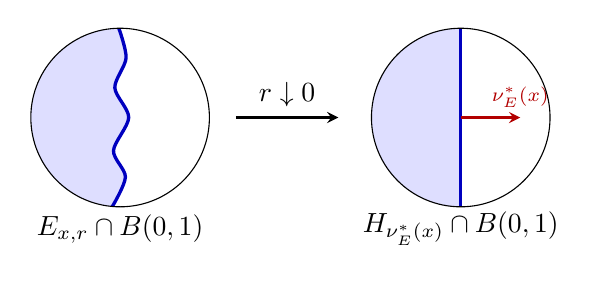
\begin{tikzpicture}[>=stealth,scale=0.84]
  \begin{scope}[shift={(0,0)}]
    \clip (0,0) circle (1.35);
    \fill[blue!13] (-1.5,-1.5)--(-0.10,-1.5)--(-0.12,-1.3)--
      (0.08,-0.9)--(-0.10,-0.5)--(0.13,0)--(-0.08,0.45)--
      (0.09,0.9)--(-0.02,1.5)--(-1.5,1.5)--cycle;
    \draw[blue!75!black,very thick] plot[smooth] coordinates
      {(-0.12,-1.35) (0.08,-0.9) (-0.10,-0.5) (0.13,0)
       (-0.08,0.45) (0.09,0.9) (-0.02,1.35)};
  \end{scope}
  \draw (0,0) circle (1.35);
  \node at (0,-1.68) {$E_{x,r}\cap B(0,1)$};
  \draw[->,thick] (1.75,0)--(3.3,0)
    node[pos=.5,above] {$r\downarrow0$};
  \begin{scope}[shift={(5.15,0)}]
    \clip (0,0) circle (1.35);
    \fill[blue!13] (-1.5,-1.5) rectangle (0,1.5);
    \draw[blue!75!black,very thick] (0,-1.4)--(0,1.4);
    \draw[->,red!70!black,thick] (0,0)--(0.9,0)
      node[above,font=\scriptsize] {$\nu_E^*(x)$};
  \end{scope}
  \draw (5.15,0) circle (1.35);
  \node at (5.15,-1.68) {$H_{\nu_E^*(x)}\cap B(0,1)$};
\end{tikzpicture}

\small\emph{Schemat granicy De Giorgiego:}
po przeskalowaniu przy punkcie brzegu zredukowanego
zbiór staje się półprzestrzenią w sensie zbieżności
$L^1_{\mathrm{loc}}$; rysunek nie oznacza zbieżności
brzegów w odległości Hausdorffa.
\end{center}

\begin{uwaga}[Brzeg topologiczny a zredukowany]
Twierdzenie nie orzeka, że $\partial E=\partial^*E$.
Zmiana $E$ na zbiorze $\lambda_n$-zerowym może
zupełnie zmienić jego brzeg topologiczny,
lecz nie zmienia $D\chi_E$, obwodu ani wzoru
Gaussa--Greena. W szczególności właściwą
miarą powierzchniową dla ogólnych zbiorów
skończonego obwodu jest
$\mathcal H^{n-1}\llcorner\partial^*E$.
\end{uwaga}

\begin{lemat}[Mierzalność obwodów zbiorów nad- i podpoziomicowych]
\label{lem:BV-level-meas-auditVI}
Niech $\Omega\subseteq\mathbb R^n$ będzie zbiorem otwartym,
a $u:\Omega\to\mathbb R$ będzie mierzalna
w sensie Lebesgue'a. Dla $t\in\mathbb R$ oznaczmy
$E_t=\{x\in\Omega:u(x)>t\}$ oraz
$F_t=\{x\in\Omega:u(x)<-t\}$.
Obie funkcje $t\mapsto P(E_t;\Omega)$ i
$t\mapsto P(F_t;\Omega)$ o wartościach
w $[0,+\infty]$ są borelowskie.
Nie zakładamy całkowalności $u$ ani skończoności
obwodów. Wartości tych funkcji nie zmieniają się
po zmianie $u$ na zbiorze miary Lebesgue'a zero.
\end{lemat}
\begin{proof}
Jeśli $\Omega=\varnothing$, oba obwody są zerowe.
W przeciwnym razie wybieramy wyczerpanie
$\Omega$ zbiorami zwartymi $(K_j)_{j\ge1}$
takie, że $K_j\subseteq\operatorname{int}K_{j+1}$.
Niech $\mathcal A_j$ oznacza zbiór pól
$\varphi\in C_c^1(\Omega;\mathbb R^n)$
o nośniku zawartym w $K_j$ i
$|\varphi(x)|\le1$ dla każdego $x$.
Wyposażamy go w metrykę normy $C^1$:
sumy norm supremum składowych i ich pierwszych
pochodnych. Odwzorowanie przypisujące polu
ograniczenia tych funkcji do $K_j$ zanurza
$\mathcal A_j$ izometrycznie w skończonym
produkcie przestrzeni $C(K_j;\mathbb R)$.
Istotnie, składowe i ich pochodne znikają
poza $K_j$, więc wystarczy mierzyć ich normy
na $K_j$. Przestrzeń $C(K_j;\mathbb R)$
jest ośrodkowa: wielomiany o współczynnikach
wymiernych tworzą przeliczalną rodzinę gęstą
na mocy twierdzenia Stone'a--Weierstrassa.
Skończony produkt przestrzeni metrycznych
ośrodkowych jest ośrodkowy, a każda jego
podprzestrzeń również jest ośrodkowa
(dziedziczy drugi aksjomat przeliczalności,
a wybór punktu z każdego niepustego elementu
przeliczalnej bazy daje zbiór gęsty).
Wybieramy więc przeliczalny gęsty podzbiór
$\mathcal D_j$ samego $\mathcal A_j$.
W szczególności każdy wybrany test już spełnia
ograniczenie punktowe normy; nie trzeba go
ponownie skalować.

Niech $\mathcal D=\{0\}\cup\bigcup_j
(\mathcal D_j\cup(-\mathcal D_j))$.
Jest to przeliczalna symetryczna rodzina
dopuszczalnych pól, którą wyliczamy jako
$(\varphi_l)_{l\ge1}$, z powtórzeniami w razie
potrzeby. Dla każdego mierzalnego $E\subseteq\Omega$
zachodzi
\[
 P(E;\Omega)=\sup_{l\ge1}
 \int_E\operatorname{div}\varphi_l(x)
 \,\mathrm d\lambda_n(x).
\]
Nierówność z prawą stroną nie większą od lewej
wynika z dopuszczalności testów.
Dla nierówności odwrotnej ustalamy dowolny test
$\varphi$ z definicji obwodu. Jego zwarty nośnik
jest zawarty w pewnym $K_j$, więc istnieją
$\psi_m\in\mathcal D_j$ z $\psi_m\to\varphi$
w normie $C^1$. Wszystkie dywergencje znikają
poza $K_j$, a zatem
\[
 \left|\int_E\operatorname{div}(\psi_m-\varphi)
 \,\mathrm d\lambda_n\right|
 \le\lambda_n(K_j)
 \|\operatorname{div}(\psi_m-\varphi)\|_\infty
 \longrightarrow0.
\]
Całka dla $\varphi$ nie przekracza zatem
supremum po $\mathcal D$. Biorąc supremum
po wszystkich $\varphi$, otrzymujemy równość,
także gdy obwód jest nieskończony.
Rodzina nie zależy od $E$ ani od $t$.

Dla ustalonego $l$ rozkładamy
$\operatorname{div}\varphi_l=g_l^+-g_l^-$,
gdzie $g_l^\pm$ są nieujemnymi funkcjami
całkowalnymi. Dla każdego znaku funkcja
\[
 t\longmapsto\int_{E_t}g_l^\pm(x)\,
 \mathrm d\lambda_n(x)
\]
jest skończona i nierosnąca, ponieważ
$E_{t_2}\subseteq E_{t_1}$ przy $t_1<t_2$.
Jest zatem borelowska. Jej różnica z analogiczną
funkcją dla drugiego znaku jest borelowska,
a supremum przeliczalnie wielu takich różnic
daje borelowskość $t\mapsto P(E_t;\Omega)$.
Rodzina $F_t$ również maleje przy wzroście $t$,
więc ten sam argument stosujemy do $F_t$.
Nie korzystamy tutaj z borelowskości $u$
ani z twierdzenia o mierzalności całek
parametrycznych: wystarcza monotoniczność
całek z nieujemnych funkcji.

Jeśli $u=\widetilde u$ prawie wszędzie, to dla
każdego $t$ odpowiednie zbiory nad- i podpoziomicowe różnią
się co najwyżej na jednym ustalonym zbiorze
miary Lebesgue'a zero. Z Lematu~\ref{lem:perimeter-complement-29}
ich obwody są równe. Dowodzi to ostatniej tezy.
\end{proof}

\section{Koobszar, funkcje BV i warstwowanie}
\begin{twierdzenie}[Jedna nierówność formuły koobszaru dla $BV$]
\label{thm:BV-layercake-29}
Niech $\Omega\subseteq\mathbb R^n$ będzie zbiorem otwartym,
$u\in L^1(\Omega;\mathbb R)$ oraz dla $t>0$
niech $E_t^+=\{x\in\Omega:u(x)>t\}$ i
$E_t^-=\{x\in\Omega:u(x)<-t\}$.
Jeśli
\[
 \int_0^\infty\!P(E_t^+;\Omega)\,\mathrm d\lambda_1(t)
 +\int_0^\infty\!P(E_t^-;\Omega)\,\mathrm d\lambda_1(t)<\infty,
\]
to $u\in BV(\Omega)$ i
\[
 |Du|(\Omega)\le\int_0^\infty
 [P(E_t^+;\Omega)+P(E_t^-;\Omega)]\,
 \mathrm d\lambda_1(t)
 =\int_{\mathbb R}P(\{u>s\};\Omega)
 \,\mathrm d\lambda_1(s).
\]
W szczególności założenie całkowe samo pociąga
skończoność obu obwodów dla prawie wszystkich $t>0$.
\end{twierdzenie}
\begin{proof}
Wybieramy wszędzie skończony borelowski
reprezentant $u$; poprzedni lemat zapewnia,
że nie zmienia to żadnego z obwodów.
Dla każdej liczby $a\in\mathbb R$ zachodzi
$\int_0^\infty\chi_{\{a>t\}}\,\mathrm d\lambda_1(t)
=\max\{a,0\}$ oraz
$\int_0^\infty\chi_{\{a<-t\}}\,\mathrm d\lambda_1(t)
=\max\{-a,0\}$. Odejmując te równości dla
$a=u(x)$, otrzymujemy punktowo wzór warstwowania
\[
 u(x)=\int_0^\infty
 \bigl(\chi_{E_t^+}(x)-\chi_{E_t^-}(x)\bigr)
 \,\mathrm d\lambda_1(t).
\]
Funkcje charakterystyczne na przestrzeni
$\Omega\times(0,\infty)$ są borelowskie.
Ponieważ dla $t>0$ zbiory $E_t^+,E_t^-$
są rozłączne, z Tonellego otrzymujemy
\begin{align*}
 \int_0^\infty\int_\Omega
 (\chi_{E_t^+}(x)+\chi_{E_t^-}(x))
 \,\mathrm d\lambda_n(x)\,\mathrm d\lambda_1(t)
 &=\int_\Omega|u(x)|\,\mathrm d\lambda_n(x)<\infty.
\end{align*}
Dla dowolnego $\varphi\in C_c^1(\Omega;\mathbb R^n)$
z $|\varphi|\le1$ całka z modułu funkcji
$(\chi_{E_t^+}-\chi_{E_t^-})\operatorname{div}\varphi$
na przestrzeni produktowej nie przekracza
$\|\operatorname{div}\varphi\|_\infty\|u\|_{L^1}$.
Spełnione są więc hipotezy Fubiniego.
Otrzymujemy
\[
 \int_\Omega u(x)\operatorname{div}\varphi(x)
 \,\mathrm d\lambda_n(x)
 =\int_0^\infty\!\left(
 \int_{E_t^+}\operatorname{div}\varphi(x)
 \,\mathrm d\lambda_n(x)
 -\int_{E_t^-}\operatorname{div}\varphi(x)
 \,\mathrm d\lambda_n(x)\right)\mathrm d\lambda_1(t).
\]
Dla każdego $t>0$ moduł pierwszej całki
w nawiasie nie przekracza $P(E_t^+;\Omega)$,
a moduł drugiej nie przekracza $P(E_t^-;\Omega)$:
w definicji obwodu dopuszczalne są oba pola
$\varphi$ i $-\varphi$.
Całka po $t$ z sumy obwodów jest dobrze
określona dzięki poprzedniemu lematowi.
Otrzymujemy oszacowanie niezależne od pola
testowego. Biorąc supremum po wszystkich
dopuszczalnych polach, dostajemy pierwszą
nierówność. Jej prawa strona jest skończona
z założenia, więc $u\in BV(\Omega)$.

Pozostaje uzasadnić przejście od dodatnich
i ujemnych warstw do całki po całej prostej.
Zbiory $\{u=-t\}$ są parami rozłączne dla
różnych $t>0$. Ponieważ $\lambda_n$ na $\Omega$
jest $\sigma$-skończona, co najwyżej przeliczalnie
wiele z tych zbiorów ma dodatnią miarę:
na każdym zbiorze wyczerpania o skończonej mierze
tylko skończenie wiele rozłącznych poziomic
może mieć miarę co najmniej $1/k$, dla
ustalonego $k\ge1$. Bierzemy sumę po wyczerpaniu
i po $k$. Dla pozostałych $t>0$ zbiory
$\{u<-t\}$ i $\{u\le-t\}$ są równe prawie wszędzie.
Drugi z nich jest dopełnieniem $\{u>-t\}$
w $\Omega$. Lemat~\ref{lem:perimeter-complement-29}
(dla dopełnień w $\mathbb R^n$ ograniczonych
do $\Omega$) daje
$P(E_t^-;\Omega)=P(\{u>-t\};\Omega)$
dla prawie wszystkich $t>0$.
Zamiana zmiennej $s=-t$ w całce z obwodów
ujemnych warstw daje równość obu wyrażeń
w tezie. Nie jest przy tym wymagana skończona
miara samego $\Omega$.
\end{proof}

\section{Pełna formuła koobszaru dla funkcji \texorpdfstring{$BV$}{BV}}
Związek między obwodem zbiorów nadpoziomicowych a wariacją
funkcji nie wymaga twierdzenia strukturalnego De Giorgiego.
Wystarczą ścisła aproksymacja w $BV$, gładki wzór
koobszaru z Rozdziału~\ref{ch:area-coarea-28} i dolna
półciągłość wariacji.

\begin{lemat}[Ścisła aproksymacja gładka w $BV$]
\label{lem:BV-strict-approx}
Niech $n\ge1$, $\Omega\subseteq\mathbb R^n$ będzie
zbiorem otwartym, a $u\in BV(\Omega)$.
Istnieje ciąg funkcji o wartościach rzeczywistych
$u_j\in C^\infty(\Omega)\cap W^{1,1}(\Omega)$ taki, że
\[
 \|u_j-u\|_{L^1(\Omega)}\longrightarrow0,
 \qquad
 \int_\Omega|\nabla u_j(x)|\,\mathrm d\lambda_n(x)
 \longrightarrow |Du|(\Omega).
\]
Nie wymaga się regularności brzegu $\Omega$.
\end{lemat}
\begin{proof}
Jeśli $\Omega=\varnothing$, teza jest oczywista.
Zakładamy dalej, że $\Omega\ne\varnothing$.

\emph{Krok 1: lokalnie skończone otoczenia nośników.}
Wybieramy rosnące wyczerpanie $(U_i)_{i\ge1}$
zbioru $\Omega$ zbiorami otwartymi takimi, że
$\overline U_i$ jest zwarty i
$\overline U_i\subseteq U_{i+1}\subseteq\Omega$.
Możemy na przykład przyjąć
$U_i=\{x\in\Omega:|x|<i,\,
\operatorname{dist}(x,\mathbb R^n\setminus\Omega)>1/i\}$,
z konwencją odległości $+\infty$ od zbioru pustego.
Kładziemy $U_i=\varnothing$ dla $i\le0$.
Rodzina otwartych zbiorów
$V_i=U_{i+1}\setminus\overline U_{i-1}$,
$i\ge1$, pokrywa $\Omega$: dla punktu $x$
bierzemy najmniejszy indeks $m$ taki, że
$x\in U_m$. Jeżeli $x\in\overline U_{m-1}$, to $m\ge2$,
$x\notin U_{m-1}$ i
$\overline U_{m-2}\subset U_{m-1}$,
więc $x\in V_{m-1}$.
W przeciwnym przypadku $x\in V_m$.
Ponadto dla każdego zwartego $K\subseteq\Omega$
istnieje $M$ z $K\subset U_M$, a wtedy
$K\cap V_i=\varnothing$ dla $i\ge M+1$.
Rodzina $(V_i)$ jest zatem lokalnie skończona.
Każdy $V_i$ ma zwarte domknięcie w $\Omega$.

Wybieramy gładki podział jedności $(\psi_i)$
podporządkowany temu pokryciu, czyli
$\psi_i\ge0$, $\operatorname{supp}\psi_i\subset V_i$
oraz $\sum_i\psi_i=1$ na $\Omega$.
Nośniki są zwarte, ponieważ są domknięte
w $\Omega$ i zawierają się w $\overline U_{i+1}$.
Do skonstruowania takiego podziału można użyć
gładkiego podziału jedności podporządkowanego
lokalnie skończonemu pokryciu otwartemu.
Istotna jest tutaj nie tylko lokalna skończoność
samych nośników, ale również otwartych zbiorów
$V_i$, w których będziemy je powiększać.
Indeksy z $\psi_i=0$ nie wnoszą wkładu do sum.
Dla każdego pozostałego indeksu istnieje $d_i>0$
takie, że zamknięte $d_i$-otoczenie
$\operatorname{supp}\psi_i$ zawiera się w $V_i$.
Wynika to ze zwartości nośnika i otwartości $V_i$.

\emph{Krok 2: dobór lokalnych wygładzeń.}
Niech $\rho\in C_c^\infty(B(0,1))$ będzie
nieujemna i niech $\int\rho\,\mathrm d\lambda_n=1$.
Dla $\varepsilon>0$ kładziemy
$\rho_\varepsilon(x)=\varepsilon^{-n}\rho(x/\varepsilon)$.
Funkcje $f_i=\psi_i u$ i $g_i=u\nabla\psi_i$
przedłużamy przez zero poza $\Omega$.
Obie należą do $L^1(\mathbb R^n)$ (druga
ma wartości wektorowe), ponieważ odpowiednie
mnożniki są ograniczone i mają zwarte nośniki.
Dla każdego $j\ge1$ oraz każdego $i$
z niezerowym $\psi_i$ wybieramy
$0<\varepsilon_{i,j}<d_i$ tak, aby
\begin{align*}
 \|\rho_{\varepsilon_{i,j}}*f_i-f_i\|_{L^1(\mathbb R^n)}
 &<2^{-i-j},\\
 \|\rho_{\varepsilon_{i,j}}*g_i-g_i\|_{L^1(\mathbb R^n)}
 &<2^{-i-j}.
\end{align*}
Jest to możliwe dzięki zbieżności splotów w $L^1$
z dowodu Lematu~\ref{lem:BV-translation-29},
stosowanej również do każdej składowej $g_i$.
Dla $\psi_i=0$ wybieramy dowolne dodatnie
$\varepsilon_{i,j}$; oba błędy są wtedy zerowe.
Nośniki wszystkich niezerowych wygładzeń
mieszczą się w $V_i$, ponieważ jądro ma nośnik
w kuli o promieniu $\varepsilon_{i,j}$.
Definiujemy
\[
 u_j=\sum_{i=1}^\infty\rho_{\varepsilon_{i,j}}*f_i
 \quad\text{na }\Omega.
\]
Lokalna skończoność $(V_i)$ pozwala różniczkować
sumę dowolną liczbę razy, więc $u_j\in C^\infty(\Omega)$.
Ponadto z nieujemności jądra i funkcji $\psi_i$
oraz z Tonellego mamy
\[
 \sum_i\|\rho_{\varepsilon_{i,j}}*f_i\|_1
 \le\sum_i\|f_i\|_1
 =\int_\Omega |u|\sum_i\psi_i\,\mathrm d\lambda_n
 =\|u\|_{L^1(\Omega)}.
\]
Suma zatem zbiega także w $L^1$.
Ponieważ $u=\sum_i f_i$ prawie wszędzie
na $\Omega$, nierówność trójkąta i dobór
$\varepsilon_{i,j}$ dają
$\|u_j-u\|_{L^1(\Omega)}\le\sum_i2^{-i-j}=2^{-j}$.

\emph{Krok 3: kontrola gradientu.}
Niech $Du=p\,|Du|$ będzie rozkładem polarnym.
Dla każdego $i$ funkcja $f_i$, przedłużona
przez zero, należy do $BV(\mathbb R^n)$.
Istotnie, dla pola $\varphi\in
C_c^1(\mathbb R^n;\mathbb R^n)$ test
$\psi_i\varphi$ ma zwarty nośnik w $\Omega$.
Stąd
\begin{align*}
 -\int_{\mathbb R^n} f_i\operatorname{div}\varphi
 \,\mathrm d\lambda_n
 &=-\int_\Omega u\operatorname{div}(\psi_i\varphi)
 \,\mathrm d\lambda_n
 +\int_\Omega u\nabla\psi_i\cdot\varphi\,\mathrm d\lambda_n\\
 &=\int_\Omega\psi_i\varphi\cdot\mathrm dDu
 +\int_\Omega u\nabla\psi_i\cdot\varphi\,\mathrm d\lambda_n.
\end{align*}
Prawa strona reprezentuje skończoną miarę
wektorową na $\mathbb R^n$ (przedłużoną przez zero
poza $\Omega$), co dowodzi skończoności wariacji
$f_i$ i tożsamości
$Df_i=\psi_i Du+g_i\lambda_n$.
Nie przedłużamy przez zero całej funkcji $u$
jako funkcji BV, a jedynie jej lokalne iloczyny.

Z rachunku pochodnych splotów wynika
$\nabla(\rho_{\varepsilon_{i,j}}*f_i)
=\rho_{\varepsilon_{i,j}}*(\psi_i Du)
+\rho_{\varepsilon_{i,j}}*g_i$.
W każdym punkcie $\Omega$ zachodzi
$\sum_i\nabla\psi_i=0$ jako pochodna lokalnie
skończonej sumy $\sum_i\psi_i=1$.
Zatem $\sum_i g_i=0$ prawie wszędzie, w sensie
lokalnie skończonej sumy (nie zakładamy
$\sum_i\|g_i\|_1<\infty$).
Otrzymujemy
\[
 \nabla u_j
 =\sum_i\rho_{\varepsilon_{i,j}}*(\psi_i Du)
 +\sum_i(\rho_{\varepsilon_{i,j}}*g_i-g_i)
 \quad\text{prawie wszędzie na }\Omega.
\]
Pierwszą sumę szacujemy przez rozkład polarny,
nierówność trójkąta i Tonellego:
\begin{align*}
 \int_\Omega\left|\sum_i
 \rho_{\varepsilon_{i,j}}*(\psi_i Du)(x)\right|
 \,\mathrm d\lambda_n(x)
 &\le\sum_i\int_{\mathbb R^n}\int_\Omega
 \rho_{\varepsilon_{i,j}}(x-y)\psi_i(y)
 \,\mathrm d|Du|(y)\,\mathrm d\lambda_n(x)\\
 &=\sum_i\int_\Omega\psi_i(y)\,\mathrm d|Du|(y)
 =|Du|(\Omega).
\end{align*}
W szczególności suma norm $L^1$ jej składników
jest skończona. Suma norm $L^1$ składników
drugiej sumy nie przekracza $2^{-j}$ z doboru
promieni wygładzeń. Stąd
\[
 \int_\Omega|\nabla u_j|\,\mathrm d\lambda_n
 \le |Du|(\Omega)+2^{-j}.
\]
Funkcja $u_j$ jest całkowalna, a jej klasyczne
pierwsze pochodne są całkowalne. Z całkowania
przez części względem testów o zwartym nośniku
wynika, że są to również jej pochodne słabe,
więc $u_j\in W^{1,1}(\Omega)$.

\emph{Krok 4: dokładna granica wariacji.}
Dla funkcji gładkiej z całkowalnym gradientem
wariacja jest równa całce z normy gradientu
(Lemat~\ref{lem:BV-smooth-29}).
Dolna półciągłość wariacji przy zbieżności
w $L^1$ z Twierdzenia~\ref{thm:perimeter-lsc-29}
daje
\[
 |Du|(\Omega)
 \le\liminf_{j\to\infty}|Du_j|(\Omega)
 =\liminf_{j\to\infty}\int_\Omega|\nabla u_j|
 \,\mathrm d\lambda_n
 \le\limsup_{j\to\infty}\int_\Omega|\nabla u_j|
 \,\mathrm d\lambda_n
 \le|Du|(\Omega).
\]
Wszystkie nierówności są zatem równościami.
Dowód nie wykorzystuje żadnej regularności
brzegu $\Omega$. Zbieżność w $L^1$ wraz ze
zbieżnością całkowitych wariacji nazywamy
\emph{zbieżnością ścisłą w $BV$}; nie oznacza
ona na ogół zbieżności w normie przestrzeni $BV$.
Na przykład dla $u=\chi_{(0,1)}$ na $\mathbb R$
miara $Du=\delta_0-\delta_1$ jest skupiona
na dwóch punktach, podczas gdy $Du_j$ dla
gładkich $u_j\in BV$ jest bezwzględnie ciągła
względem $\lambda_1$. Miary ich wariacji
są więc wzajemnie osobliwe i
$|D(u_j-u)|(\mathbb R)=|Du_j|(\mathbb R)+2\ge2$,
choć można dobrać $u_j$ zbieżne ściśle do $u$.
\end{proof}

\begin{lemat}[Obwody zbiorów nadpoziomicowych funkcji gładkiej]
\label{lem:BV-smooth-levels}
Niech $n\ge1$, $\Omega\subseteq\mathbb R^n$ będzie
zbiorem otwartym, a $v\in C^1(\Omega;\mathbb R)$
spełnia $\int_\Omega|\nabla v(x)|\,\mathrm d\lambda_n(x)<\infty$.
Dla $t\in\mathbb R$ oznaczmy $E_t=\{x\in\Omega:v(x)>t\}$.
Wówczas dla $\lambda_1$-prawie każdego $t$
zbiór $E_t$ ma skończony obwód w $\Omega$ oraz
jako miary wektorowe na $\Omega$ zachodzi
\[
 D\chi_{E_t}=
 \frac{\nabla v}{|\nabla v|}\,
 \mathcal H^{n-1}\llcorner
 \{x\in\Omega:v(x)=t,\ \nabla v(x)\ne0\}.
\]
Ponadto
\[
 \int_{-\infty}^{\infty}P(\{v>t\};\Omega)
 \,\mathrm d\lambda_1(t)
 \le\int_\Omega|\nabla v(x)|\,\mathrm d\lambda_n(x).
\]
\end{lemat}
\begin{proof}
Wybierzmy gładką, niemalejącą funkcję
$\theta:\mathbb R\to[0,1]$, równą $0$ na
$(-\infty,0]$ i $1$ na $[1,\infty)$, i niech
$\theta_\varepsilon(s)=\theta(s/\varepsilon)$.
Dla pola $\varphi\in C_c^1(\Omega;\mathbb R^n)$
całkowanie przez części daje
\[
 \int_\Omega\theta_\varepsilon(v(x)-t)
 \operatorname{div}\varphi(x)\,\mathrm d\lambda_n(x)
 =-\int_\Omega\theta'_\varepsilon(v(x)-t)
 \nabla v(x)\cdot\varphi(x)\,\mathrm d\lambda_n(x).
\]
Dla każdego $x$ i każdego $t$ funkcja
$\theta_\varepsilon(v(x)-t)$ zbiega do
$\chi_{E_t}(x)$, również gdy $v(x)=t$,
ponieważ $\theta(0)=0$. Całkowanie odbywa się
na zwartym nośniku dywergencji pola testowego,
więc twierdzenie o zbieżności zdominowanej
daje granicę $\int_{E_t}\operatorname{div}\varphi$
dla każdego $t$. Nie trzeba wykluczać poziomic
o dodatniej mierze Lebesgue'a.
Z kolei wzór koobszaru dla odwzorowania
$v:\Omega\to\mathbb R$ pozwala zapisać
prawą stronę jako
\[
 -\int_{\mathbb R}\theta'_\varepsilon(s-t)
 \left(\int_{\{v=s,\,\nabla v\ne0\}}
 \frac{\nabla v(x)}{|\nabla v(x)|}\cdot\varphi(x)
 \,\mathrm d\mathcal H^{n-1}(x)\right)
 \,\mathrm d\lambda_1(s).
\]
Wzór koobszaru stosujemy do borelowskich
funkcji wagowych, rozdzielając części dodatnią
i ujemną iloczynu skalarnego. Na dowolnym
wyczerpaniu zbiorami względnie zwartymi
odwzorowanie $v$ jest lokalnie Lipschitzowskie;
wzór z Rozdziału~\ref{ch:area-coarea-28}
można stosować na przeliczalnym pokryciu
kulami o zwartych domknięciach w $\Omega$,
a następnie sumować po rozłącznych borelowskich
fragmentach tych kul. W szczególności funkcja
$M(t)=\mathcal H^{n-1}(\{v=t,\nabla v\ne0\})$
jest mierzalna względem $\lambda_1$ i
$\int_{\mathbb R}M(t)\,\mathrm d\lambda_1(t)
=\int_\Omega|\nabla v|\,\mathrm d\lambda_n<\infty$.
Oznaczmy funkcję w nawiasie przez $F_\varphi(s)$.
Jest ona mierzalna względem $\lambda_1$,
a jej moduł jest ograniczony przez
$\|\varphi\|_\infty M(s)$, zatem należy do $L^1$.
Wartości na zbiorze wyjątkowym, na którym
całka powierzchniowa nie jest skończona,
ustalamy jako zero.
Ponieważ $\theta'\ge0$, jej nośnik leży
w $[0,1]$, a całka wynosi $1$,
$\theta'_\varepsilon(s-t)$ jest jądrem
jednostronnej średniej. W każdym punkcie
Lebesgue'a $t$ funkcji $F_\varphi$ mamy
\[
 \left|\int_{\mathbb R}\theta'_\varepsilon(s-t)
 F_\varphi(s)\,\mathrm d\lambda_1(s)-F_\varphi(t)\right|
 \le\frac{\|\theta'\|_\infty}{\varepsilon}
 \int_t^{t+\varepsilon}|F_\varphi(s)-F_\varphi(t)|
 \,\mathrm d\lambda_1(s)\longrightarrow0.
\]
Twierdzenie Lebesgue'a o różniczkowaniu daje
zatem dla prawie wszystkich $t$
\[
 \int_{\{v>t\}}\operatorname{div}\varphi(x)
 \,\mathrm d\lambda_n(x)
 =-\int_{\{v=t,\,\nabla v\ne0\}}
 \frac{\nabla v(x)}{|\nabla v(x)|}\cdot\varphi(x)
 \,\mathrm d\mathcal H^{n-1}(x).
\]
Aby uzyskać jeden zbiór poziomów dla wszystkich
testów, stosujemy konstrukcję ośrodkowości
z dowodu Lematu~\ref{lem:BV-level-meas-auditVI},
tym razem bez ograniczenia normy pól.
Na każdym zwartym zbiorze wyczerpania
wybieramy przeliczalną rodzinę gęstą w normie
$C^1$ w przestrzeni pól o nośniku w tym zbiorze.
Usuwamy z prostej zbiór zerowy, na którym
$M(t)=+\infty$, oraz zbiory wyjątkowe
dla wszystkich pól z sumy tych rodzin.
Dla każdego pozostałego $t$ równość zachodzi
dla całej przeliczalnej rodziny. Lewa strona
jest ciągła w normie $C^1$ na ustalonym
zwartym nośniku, a prawa w normie supremum,
z oszacowaniem przez $M(t)$ razy normę pola.
Równość przenosi się zatem na dowolny test.
Prawa strona reprezentuje, z uwzględnieniem
znaku w definicji pochodnej dystrybucyjnej,
miarę wektorową z tezy. Jest ona skończona,
a jej gęstość względem miary powierzchniowej
ma normę $1$. Z twierdzenia o reprezentacji
pochodnej i wariacji otrzymujemy
$P(E_t;\Omega)=M(t)$ dla tych poziomów.
Zatem nawet równość całek zachodzi w podanym
oszacowaniu. Dowód nie wymaga twierdzenia
Sarda ani tego, aby $v$ należała do $L^1(\Omega)$.
\end{proof}

\begin{twierdzenie}[Pełna formuła koobszaru dla $BV$]
\label{thm:BV-coarea-full-29}
Niech $\Omega\subseteq\mathbb R^n$ będzie zbiorem otwartym.
Jeżeli $u\in BV(\Omega)$, to dla prawie wszystkich
$t\in\mathbb R$ zbiór $\{x\in\Omega:u(x)>t\}$
ma skończony obwód w $\Omega$ oraz
\begin{equation}\label{eq:BV-coarea-full-29}
 |Du|(\Omega)=\int_{-\infty}^{\infty}
 P(\{u>t\};\Omega)\,\mathrm d\lambda_1(t).
\end{equation}
W szczególności dla każdego $u\in BV_{\mathrm{loc}}(\Omega)$
i otwartego $V\subseteq\Omega$ zachodzi równość,
być może z dwiema stronami równymi $+\infty$,
\[
 |Du|(V)=\int_{-\infty}^{\infty}
 P(\{u>t\};V)\,\mathrm d\lambda_1(t).
\]
\end{twierdzenie}
\begin{proof}
Najpierw niech $u\in BV(\Omega)$.
Wybierzmy z Lematu~\ref{lem:BV-strict-approx}
ciąg $u_j\in C^\infty(\Omega)\cap W^{1,1}(\Omega)$
zbiegający do $u$ w $L^1$, ze zbieżnością
całek z gradientu do $|Du|(\Omega)$.
Z konstrukcji w Lemacie~\ref{lem:BV-strict-approx}
możemy przyjąć $\|u_j-u\|_{L^1}\le2^{-j}$,
więc $\sum_j\|u_j-u\|_{L^1}<\infty$.
Wybieramy skończony borelowski reprezentant $u$,
bez zmiany żadnego obwodu.
Dla $a,b\in\mathbb R$ obie funkcje
$t\mapsto\chi_{\{a>t\}}$ i
$t\mapsto\chi_{\{b>t\}}$ różnią się na
przedziale między $a$ i $b$, z ewentualną
różnicą na końcach. Dlatego tożsamość liczbowa
$\int_{\mathbb R}|\chi_{\{a>t\}}-
\chi_{\{b>t\}}|\,\mathrm d\lambda_1(t)=|a-b|$
i twierdzenie Tonellego dają
\[
 \int_{\mathbb R}\|\chi_{\{u_j>t\}}-
 \chi_{\{u>t\}}\|_{L^1(\Omega)}
 \,\mathrm d\lambda_1(t)=\|u_j-u\|_{L^1(\Omega)}.
\]
Niech $a_j(t)$ oznacza całkę z modułu różnicy
funkcji charakterystycznych po $\Omega$.
Z Tonellego i powyższej tożsamości
$\int_{\mathbb R}\sum_j a_j(t)\,\mathrm d\lambda_1(t)
=\sum_j\|u_j-u\|_1<\infty$.
Zatem dla prawie wszystkich $t$ wszystkie
$a_j(t)$ są skończone i $a_j(t)\to0$.
W szczególności funkcje charakterystyczne
zbiegają w $L^1_{\rm loc}(\Omega)$.
Nie twierdzimy, że każda z nich należy
do globalnego $L^1(\Omega)$: dla ujemnych
poziomów i zbioru $\Omega$ o nieskończonej
mierze może to być fałszywe.
Półciągłość obwodu,
Lemat~\ref{lem:BV-level-meas-auditVI},
nierówność Fatou i Lemat~\ref{lem:BV-smooth-levels}
dają
\begin{align*}
 \int_{\mathbb R}P(\{u>t\};\Omega)\,
 \mathrm d\lambda_1(t)
 &\le\liminf_j\int_{\mathbb R}
 P(\{u_j>t\};\Omega)\,\mathrm d\lambda_1(t)\\
 &\le\liminf_j\int_\Omega|\nabla u_j(x)|
 \,\mathrm d\lambda_n(x)=|Du|(\Omega).
\end{align*}
W szczególności dla prawie wszystkich $t$
zbiór nadpoziomicowy ma skończony obwód.

Otrzymana skończoność całki jest dokładnie
założeniem Twierdzenia~\ref{thm:BV-layercake-29},
w którym wykazano również równość całki
po całej prostej z sumą całek po dodatnich
i ujemnych warstwach. Stosując to twierdzenie
do $u\in L^1(\Omega)$, dostajemy
$|Du|(\Omega)\le\int_{\mathbb R}
P(\{u>t\};\Omega)\,\mathrm d\lambda_1(t)$.
To kończy dowód równości.

Dla $u\in BV_{\mathrm{loc}}(\Omega)$ i otwartego
$V\subseteq\Omega$ wybieramy wyczerpanie $V$
przez rosnące zbiory otwarte $V_j$ o zwartych
domknięciach w $\Omega$. Na każdym $V_j$
funkcja $u$ jest całkowalna i ma skończoną
wariację; stosujemy właśnie udowodnioną równość.
Mamy $|Du|(V_j)\uparrow|Du|(V)$ z ciągłości
miary od dołu. Dla każdego $t$, również
wyjątkowego, zachodzi
$P(\{u>t\};V_j)\uparrow P(\{u>t\};V)$:
obwody są niemalejące z rozszerzaniem klasy
testów, a każde pole o zwartym nośniku w $V$
ma nośnik zawarty w pewnym $V_j$.
Supremum po wszystkich testach w $V$
jest zatem supremum po rosnącej rodzinie
klas testowych w $V_j$.
Lemat~\ref{lem:BV-level-meas-auditVI}
zapewnia mierzalność funkcji obwodu
dla każdego $V_j$ i dla $V$.
Twierdzenie o zbieżności monotonicznej
daje tezę, także gdy wspólna wartość
obu stron wynosi $+\infty$.
\end{proof}

\begin{wniosek}[Wzór koobszaru z wagą]
\label{cor:BV-coarea-weighted-29}
Niech $n\ge1$, $\Omega\subseteq\mathbb R^n$
będzie zbiorem otwartym i $u\in BV_{\mathrm{loc}}(\Omega)$.
Dla prawie wszystkich $t\in\mathbb R$ funkcja
$\chi_{\{u>t\}}$ należy do $BV_{\mathrm{loc}}(\Omega)$.
Dla pozostałych $t$ przyjmujemy w całce po $t$
miarę zerową zamiast niezdefiniowanej wariacji.
Dla każdej borelowskiej $g:\Omega\to[0,+\infty]$
zachodzi
\[
 \int_\Omega g(x)\,\mathrm d|Du|(x)
 =\int_{\mathbb R}\left(\int_\Omega g(x)
 \,\mathrm d|D\chi_{\{u>t\}}|(x)\right)
 \,\mathrm d\lambda_1(t).
\]
\end{wniosek}
\begin{proof}
Wybieramy rosnące wyczerpanie $\Omega$
otwartymi zbiorami $V_j$ o zwartych domknięciach
w $\Omega$. Na mocy Twierdzenia~\ref{thm:BV-coarea-full-29}
oraz Lematu~\ref{lem:BV-level-meas-auditVI}
zbiór
\[
 T=\bigcap_{j=1}^\infty
 \{t\in\mathbb R:P(\{u>t\};V_j)<\infty\}
\]
jest borelowski i ma dopełnienie miary zero.
Dla $t\in T$ funkcja charakterystyczna
zbioru nadpoziomicowego jest lokalnie całkowalna
i ma skończoną wariację na każdym $V_j$.
Każdy względnie zwarty otwarty podzbiór $\Omega$
zawiera się w pewnym $V_j$, więc funkcja ta
należy do $BV_{\rm loc}(\Omega)$.
Definiujemy dodatnią lokalnie skończoną
miarę Radona $\mu_t$ na $\Omega$ przez
$\mu_t=|D\chi_{\{u>t\}}|$ dla $t\in T$,
a $\mu_t=0$ dla $t\notin T$.

Dla każdego otwartego $V\subseteq\Omega$
funkcja $t\mapsto\mu_t(V)$ jest borelowska:
na $T$ jest równa $P(\{u>t\};V)$,
a poza $T$ jest zerowa.
Uzasadnimy rozszerzenie tej mierzalności
na wszystkie zbiory borelowskie.
Ustalmy $j$ i rozważmy klasę $\mathcal L_j$
borelowskich podzbiorów $A\subseteq V_j$,
dla których $t\mapsto\mu_t(A)$ jest borelowska.
Mamy $V_j\in\mathcal L_j$, a $\mu_t(V_j)$
jest skończona dla każdego $t$ z definicji $T$
i zerowego przedłużenia.
Jeżeli $A\in\mathcal L_j$, to
$\mu_t(V_j\setminus A)=\mu_t(V_j)-\mu_t(A)$,
więc również $V_j\setminus A\in\mathcal L_j$.
Dla ciągu parami rozłącznych zbiorów z
$\mathcal L_j$ ich suma należy do $\mathcal L_j$,
ponieważ jej masa jest sumą nieujemnych
funkcji borelowskich.
Jest to zatem układ Dynkina.
Zawiera rodzinę wszystkich względnie otwartych
podzbiorów $V_j$, zamkniętą na skończone
przecięcia, która generuje borelowskie zbiory
$V_j$. Twierdzenie o układach $\pi$ i $\lambda$
daje $\mathcal L_j=\mathcal B(V_j)$.
Dla dowolnego borelowskiego $A\subseteq\Omega$
mamy $\mu_t(A)=\lim_j\mu_t(A\cap V_j)$
z ciągłości od dołu, więc $t\mapsto\mu_t(A)$
jest borelowska.

Definiujemy na borelowskich zbiorach $\Omega$
$\eta(A)=\int_{\mathbb R}\mu_t(A)\,\mathrm d\lambda_1(t)$.
Mamy $\eta(\varnothing)=0$, a dla rozłącznych
borelowskich $A_i$ addytywność $\mu_t$
i twierdzenie o zbieżności monotonicznej dają
\[
 \eta\Bigl(\bigcup_iA_i\Bigr)
 =\int_{\mathbb R}\sum_i\mu_t(A_i)\,\mathrm d\lambda_1(t)
 =\sum_i\eta(A_i).
\]
Zatem $\eta$ jest miarą. Dla otwartego $V$
pominięcie $\mathbb R\setminus T$ nie zmienia
całki z nieujemnej funkcji obwodu, więc
Twierdzenie~\ref{thm:BV-coarea-full-29} daje
$\eta(V)=|Du|(V)$.
W szczególności $\eta(V_j)<\infty$.
Na każdym $V_j$ ograniczenia obu miar są
skończone i zgadzają się na względnie otwartych
podzbiorach, które tworzą układ $\pi$
generujący zbiory borelowskie. Z jednoznaczności
miar skończonych wynika ich zgodność na
$\mathcal B(V_j)$. Przechodząc do granicy
po wyczerpaniu dostajemy $\eta=|Du|$ na
$\mathcal B(\Omega)$.

Dla nieujemnej borelowskiej funkcji prostej
$g=\sum_{i=1}^m a_i\chi_{A_i}$ z nieujemnymi
skończonymi współczynnikami $a_i$ równość
z tezy wynika z liniowości dla skończonych
sum nieujemnych całek i tożsamości miar
$\eta(A_i)=|Du|(A_i)$. Funkcja
$t\mapsto\int g\,\mathrm d\mu_t$ jest wtedy
borelowska. Dla dowolnej nieujemnej borelowskiej
$g$ wybieramy rosnący ciąg nieujemnych funkcji
prostych $g_m\uparrow g$. Zbieżność monotoniczna
najpierw względem $\mu_t$ daje
$\int g_m\,\mathrm d\mu_t\uparrow\int g\,\mathrm d\mu_t$
dla każdego $t$, stąd mierzalność całki wewnętrznej.
Następnie zbieżność monotoniczna względem
$\lambda_1$ i $|Du|$ daje żądaną równość
także dla całek nieskończonych.
\end{proof}

\begin{przyklad}[Funkcja ze skokiem i formuła koobszaru]
Niech $\Omega=(-2,2)$ i $u=\chi_{(0,1)}$.
Wtedy $Du=\delta_0-\delta_1$ jako miara
ze znakiem, zatem $|Du|(\Omega)=2$.
Dla $0\le t<1$ mamy $\{u>t\}=(0,1)$ i
$P(\{u>t\};\Omega)=2$.
Dla $t<0$ zbiór nadpoziomicowy jest równy
$\Omega$, a dla $t\ge1$ jest pusty; w obu
przypadkach obwód względny w $\Omega$ wynosi zero. Stąd
$\int_{\mathbb R}P(\{u>t\};\Omega)
\,\mathrm d\lambda_1(t)=\int_0^1 2\,
\mathrm d\lambda_1(t)=2$, zgodnie z
Twierdzeniem~\ref{thm:BV-coarea-full-29}.
\end{przyklad}

\begin{przyklad}[Gęsta zmiana reprezentanta nie zmienia brzegu zredukowanego]
Dla $E=(0,1)^n\setminus\mathbb Q^n$
zachodzi $\chi_E=\chi_{(0,1)^n}$ prawie wszędzie.
Stąd $|D\chi_E|$ jest miarą powierzchniową
na ścianach sześcianu, a jego brzeg zredukowany
zgadza się z sumą wnętrz ścian, z dokładnością
do zbioru $\mathcal H^{n-1}$-zerowego.
Natomiast brzeg topologiczny $E$ zawiera
cały domknięty sześcian, ponieważ zarówno
$E$, jak i jego dopełnienie są gęste
wewnątrz $[0,1]^n$. To pokazuje, że
brzeg topologiczny nie może zastępować
$\partial^*E$ w twierdzeniu De Giorgiego.
\end{przyklad}

\section{Elementy teorii prądów}
\begin{definicja}[Prąd i jego brzeg]
\label{def:current-29}
Niech $n\ge1$, $\Omega\subseteq\mathbb R^n$
będzie zbiorem otwartym i $0\le k\le n$.
Przez $\mathcal D^k(\Omega)$ oznaczamy przestrzeń
gładkich rzeczywistych $k$-form o zwartym nośniku.
W standardowych współrzędnych zapisujemy
$\omega=\sum_I\omega_I\,\mathrm dx^I$, gdzie
$I=(i_1,\ldots,i_k)$ przebiega rosnące układy
indeksów, a $\mathrm dx^I=\mathrm dx^{i_1}\wedge
\cdots\wedge\mathrm dx^{i_k}$. Dla $k=0$
jest to po prostu przestrzeń funkcji testowych.
Nośnik formy jest sumą nośników jej współczynników.

Dla zwartego $K\subseteq\Omega$ i liczby
całkowitej $m\ge0$ kładziemy
\[
 p_{K,m}(\omega)=
 \max_{I,\ |\alpha|\le m}\sup_{x\in K}
 |\partial^\alpha\omega_I(x)|,
\]
gdzie $\alpha\in\mathbb N_0^n$ jest wielowskaźnikiem.
Na formach o nośniku w ustalonym $K$ używamy
topologii wyznaczonej przez te półnormy, a na
całym $\mathcal D^k(\Omega)$ topologii
lokalnie wypukłej granicy induktywnej tych
przestrzeni przy zwartym wyczerpaniu $\Omega$.

\emph{Prądem wymiaru $k$} nazywamy ciągły
rzeczywisty funkcjonał liniowy
$T:\mathcal D^k(\Omega)\to\mathbb R$.
Równoważnie, dla każdego zwartego $K\subseteq\Omega$
istnieją $C_K>0$ oraz całkowite $m_K\ge0$ takie, że
\[
 |T(\omega)|\le C_Kp_{K,m_K}(\omega)
 \qquad(\operatorname{supp}\omega\subseteq K).
\]
Jeśli $T$ jest prądem wymiaru $k\ge1$, jego
\emph{brzeg} definiujemy przez
$(\partial T)(\omega)=T(\mathrm d\omega)$
dla $\omega\in\mathcal D^{k-1}(\Omega)$.
Dla $k=0$ przyjmujemy brzeg równy zeru
w zerowej przestrzeni prądów wymiaru $-1$.
\end{definicja}

\begin{uwaga}[Ciągłość i wymiar brzegu]
Kryterium półnormowe z definicji wynika z tego,
że ciągłość funkcjonału na przestrzeni form
o nośniku w $K$ oznacza ograniczoność przez
skończenie wiele półnorm, które można zastąpić
jedną, ponieważ $p_{K,m}$ rośnie wraz z $m$.
Dokładniej, z ciągłości w zerze istnieją
$m$ i $\delta>0$, dla których
$p_{K,m}(\omega)<\delta$ pociąga
$|T(\omega)|<1$. Skalowanie daje
$|T(\omega)|\le 2p_{K,m}(\omega)/\delta$,
a gdy półnorma jest zerowa, skalowanie
dowolnym czynnikiem daje $T(\omega)=0$.
Odwrotnie, takie oszacowania zapewniają
ciągłość ograniczeń do przestrzeni o ustalonym
zwartym nośniku, a własność definiująca
lokalnie wypukłą granicę induktywną
zapewnia ciągłość funkcjonału na całej
przestrzeni testowej.
\end{uwaga}

\begin{lemat}[Brzeg brzegu znika]
\label{lem:current-boundary-square-29}
Niech $\Omega\subseteq\mathbb R^n$ będzie zbiorem otwartym,
$n\ge1$, $1\le k\le n$, a $T$ będzie prądem
wymiaru $k$ na $\Omega$. Wtedy $\partial T$
jest prądem wymiaru $k-1$ oraz
$\partial(\partial T)=0$ (z przyjętą konwencją
dla $k=1$).
\end{lemat}
\begin{proof}
Operator różniczki zewnętrznej jest liniowy
i nie powiększa nośnika formy. Dla testu
$\omega\in\mathcal D^{k-1}(\Omega)$ o nośniku
w $K$ współczynniki $\mathrm d\omega$
są sumami z odpowiednimi znakami pierwszych
pochodnych współczynników $\omega$.
Stąd dla każdego $m\ge0$ zachodzi
$p_{K,m}(\mathrm d\omega)\le n p_{K,m+1}(\omega)$.
Wybierając dla $T$ stałą $C_K$ i rząd $m_K$
z definicji, otrzymujemy
\[
 |(\partial T)(\omega)|
 \le C_K p_{K,m_K}(\mathrm d\omega)
 \le n C_K p_{K,m_K+1}(\omega).
\]
Funkcjonał $\partial T$ jest liniowy i spełnia
kryterium ciągłości na każdym zwartym nośniku.
Jest więc prądem wymiaru $k-1$.

Dla $k=1$ druga teza jest konsekwencją przyjętej
konwencji. Jeśli $k\ge2$, to dla
$\omega\in\mathcal D^{k-2}(\Omega)$ mamy
\[
 (\partial(\partial T))(\omega)
 =(\partial T)(\mathrm d\omega)
 =T(\mathrm d^2\omega)=0.
\]
Ostatnia równość wynika z przemienności
mieszanych pochodnych drugiego rzędu i
antysymetrii iloczynu zewnętrznego:
w wyrażeniu $\mathrm d^2\omega$ składniki
z powtórzonym indeksem znikają, a składniki
z różnymi indeksami występują parami
z przeciwnymi znakami. Z dowolności testu
wynika $\partial(\partial T)=0$.
\end{proof}

\begin{przyklad}[Prąd zadany przez powierzchnię]
Niech $\Omega\subseteq\mathbb R^n$ będzie
otwarty, $1\le k\le n$ i niech $S\subseteq\Omega$
będzie zorientowaną zwartą gładką
$k$-wymiarową podrozmaitością z brzegiem,
z orientacją brzegu indukowaną przez normalną
zewnętrzną w $TS$ (normalna zewnętrzna
jest pierwszym wektorem dodatniej bazy $TS$
na brzegu). Jeżeli $\iota:S\to\Omega$ jest
inkluzją, definiujemy
$T_S(\omega)=\int_S\iota^*\omega$.
Sprawdzimy, że jest to prąd wymiaru $k$.
Niech $\tau_S(x)$ oznacza jednostkowy prosty
$k$-wektor wyznaczający orientację $T_xS$.
Wówczas
\[
 T_S(\omega)=\int_S\omega_x(\tau_S(x))
 \,\mathrm d\mathcal H^k(x).
\]
Tożsamość wynika ze wzoru na pole dla lokalnych
parametryzacji i definicji całkowania form:
w dodatnio zorientowanej parametryzacji
iloczyn zewnętrzny wektorów stycznych jest
$\tau_S$ pomnożonym przez pierwiastek
z wyznacznika macierzy Grama.
W standardowej bazie ortonormalnej przestrzeni
$k$-wektorów współrzędne jednostkowego
$\tau_S$ mają sumę kwadratów równą $1$.
Zatem dla formy o nośniku w $K$
nierówność Cauchy'ego--Schwarza daje
\[
 |T_S(\omega)|
 \le\binom nk^{1/2}p_{K,0}(\omega)\,
 \mathcal H^k(S\cap K).
\]
Miara $\mathcal H^k(S)$ jest skończona:
zwartość $S$ pozwala wybrać skończenie wiele
lokalnych parametryzacji, również przy brzegu,
ograniczonych do zwartych fragmentów dziedzin;
na każdym z nich wzór na pole i ograniczoność
różniczki dają skończoną miarę obrazu.
Otrzymane oszacowanie dowodzi ciągłości $T_S$,
a liniowość wynika z liniowości całki.

Dla $\omega\in\mathcal D^{k-1}(\Omega)$
różniczka zewnętrzna komutuje z cofnięciem
formy przez inkluzję. Twierdzenie Stokesa,
z opisaną orientacją brzegu, daje
\[
 (\partial T_S)(\omega)
 =\int_S\mathrm d(\iota^*\omega)
 =\int_{\partial S}(\iota|_{\partial S})^*\omega
 =T_{\partial S}(\omega).
\]
Jeśli brzeg jest pusty, ostatni prąd jest zerowy.
Właśnie w tej postaci klasyczny rachunek na
rozmaitościach staje się szczególnym przypadkiem
teorii prądów. Dla przykładu na prostej,
gdy $S=[a,b]$ jest zorientowany zgodnie
z rosnącą współrzędną, dla testu $f$ mamy
$(\partial T_S)(f)=\int_a^b f'(t)\,
\mathrm d\lambda_1(t)=f(b)-f(a)$.
Stąd $\partial T_S=\delta_b-\delta_a$,
a nie $\delta_a-\delta_b$.
\end{przyklad}

\begin{przyklad}[Prąd zbioru o lokalnie skończonym obwodzie]
Niech $E\subseteq\mathbb R^n$ będzie mierzalnym
zbiorem lokalnie skończonego obwodu, a
$\Omega\subseteq\mathbb R^n$ zbiorem otwartym.
Oznaczmy standardową formę objętości przez
$\mathrm{vol}=\mathrm dx^1\wedge\cdots\wedge\mathrm dx^n$.
Definiujemy prąd wymiaru $n$ przez
$T_E(f\,\mathrm{vol})=\int_{E\cap\Omega}
f\,\mathrm d\lambda_n$.
Dla testu o nośniku w zwartym $K\subseteq\Omega$
jego wartość ma moduł nie większy niż
$\lambda_n(K)\|f\|_\infty$, więc jest to prąd
bez założenia skończonej objętości $E$.

Każdą $(n-1)$-formę testową można jednoznacznie
zapisać jako $\omega=\iota_\varphi\mathrm{vol}$,
gdzie $\varphi\in C_c^\infty(\Omega;\mathbb R^n)$,
a $\iota_\varphi$ oznacza kontrakcję przez wektor.
Współrzędnie
\[
 \omega=\sum_{i=1}^n(-1)^{i-1}\varphi_i\,
 \mathrm dx^1\wedge\cdots\wedge
 \widehat{\mathrm dx^i}\wedge\cdots\wedge\mathrm dx^n.
\]
Daszek oznacza pominięcie czynnika. Różniczkując
ten wzór, widzimy, że przeżywają tylko pochodne
$\partial_i\varphi_i$; przestawienie $\mathrm dx^i$
na właściwe miejsce daje drugi czynnik
$(-1)^{i-1}$. Dlatego
$\mathrm d\omega=(\operatorname{div}\varphi)\mathrm{vol}$.
Po przedłużeniu pola przez zero poza $\Omega$
twierdzenie strukturalne De Giorgiego daje
\[
 (\partial T_E)(\omega)
 =\int_{E\cap\Omega}\operatorname{div}\varphi\,
 \mathrm d\lambda_n
 =\int_{\partial^*E\cap\Omega}\varphi\cdot\nu_E^*
 \,\mathrm d\mathcal H^{n-1}.
\]
Znak jest zgodny z orientacją brzegu:
$(\iota_\varphi\mathrm{vol})(\tau)
=\mathrm{vol}(\varphi,\tau)$, gdzie
$\tau$ jest jednostkowym $(n-1)$-wektorem
orientującym $\nu_E^*(x)^\perp$ tak,
aby $\mathrm{vol}(\nu_E^*,\tau)=1$.
Rozkładając $\varphi$ na składową normalną
i styczną, dostajemy
$\mathrm{vol}(\varphi,\tau)=\varphi\cdot\nu_E^*$,
bo składnik styczny daje wyznacznik zerowy.
Formuła jest więc miarowym odpowiednikiem
klasycznej całki brzegowej.
Nie pojawia się tu dodatkowy wkład od
$\partial\Omega$, ponieważ testy mają nośnik
zwarty wewnątrz $\Omega$.
Na prostej dla $\Omega=\mathbb R$ i $E=(a,b)$
otrzymujemy $\partial T_E=\delta_b-\delta_a$,
podczas gdy $D\chi_E=\delta_a-\delta_b$:
znak wynika z różnych definicji obu operatorów.
\end{przyklad}

\section{Podsumowanie zależności i dalsze kierunki}
W rozdziale otrzymaliśmy reprezentację pochodnych
$BV$ przez miary, półciągłość i zwartość obwodu,
miarową formułę Gaussa--Greena, twierdzenie strukturalne
De Giorgiego wraz z geometrycznym opisem brzegu
zredukowanego oraz pełną formułę koobszaru dla $BV$.
Dowód twierdzenia strukturalnego opierał się na
nierównościach izoperymetrycznych, zwartości w $BV$,
granicach zbiorów po przeskalowaniu, prostowalności
wyprowadzonej z lokalnej płaskości oraz
identyfikacji gęstości miar. Skupienie wariacji
na brzegu zredukowanym uzyskaliśmy niezależnie
przez różniczkowanie względem miary Radona.
Dowód formuły koobszaru był niezależny od
tej struktury: wykorzystał ścisłą aproksymację
gładką i wzór koobszaru dla odwzorowań Lipschitzowskich.
Dalsze zagadnienia to m.in. dokładni reprezentanci
funkcji $BV$, twierdzenia o śladach, reguły
łańcuchowe oraz teoria powierzchni minimalnych.
Teoria prądów wiąże wzór Gaussa--Greena z operatorem
brzegu, ale nie była potrzebna do dowodu twierdzenia
strukturalnego ani wzoru koobszaru.

\begin{uwaga}[Miary wektorowe w dalszym ciągu skryptu]
Dla $u\in BV(\Omega)$ miara $Du$ ma skończoną wariację
i jest szczególnym przypadkiem miary o wartościach
w przestrzeni Banacha, omawianej w
Rozdziale~\ref{ch:vector-measures-30}.
W przypadku $u\in BV_{\mathrm{loc}}(\Omega)$ jej wariacja
jest tylko lokalnie skończona; nie musimy wtedy otrzymać
skończonego wektora $Du(\Omega)$.
Rozdział 30 interpretuje rozkład polarny poprzez RNP
przestrzeni $\mathbb R^n$. Nie należy jednak utożsamiać
tego rozkładu z istnieniem gęstości $Du$ względem
miary Lebesgue'a.
\end{uwaga}
